%!TEX encoding = UTF-8 Unicode
\documentclass[a4paper]{compendium}
\usepackage[swedish]{babel}
\addto\captionsswedish{%
  \renewcommand{\appendixname}{Appendix}%
}
%TODO: Glossary
%http://tex.stackexchange.com/questions/5821/creating-a-standalone-glossary/5837#5837

\setlength{\columnsep}{16mm}

\title{
{\vspace{-3.0cm}\bf\sffamily\Huge\selectfont  Introduktion till programmering med Scala och Java} 
\\ \vspace{1em}%\hspace*{1.5cm}\inputgraphics[width=0.6\textwidth]{../img/gurka} \\
{\sffamily  Grundkurs}\\\vspace{2cm}
%
\includegraphics[height=4cm]{../img/scala-logo.png}
%
\includegraphics[height=4cm]{../img/java-logo.png}
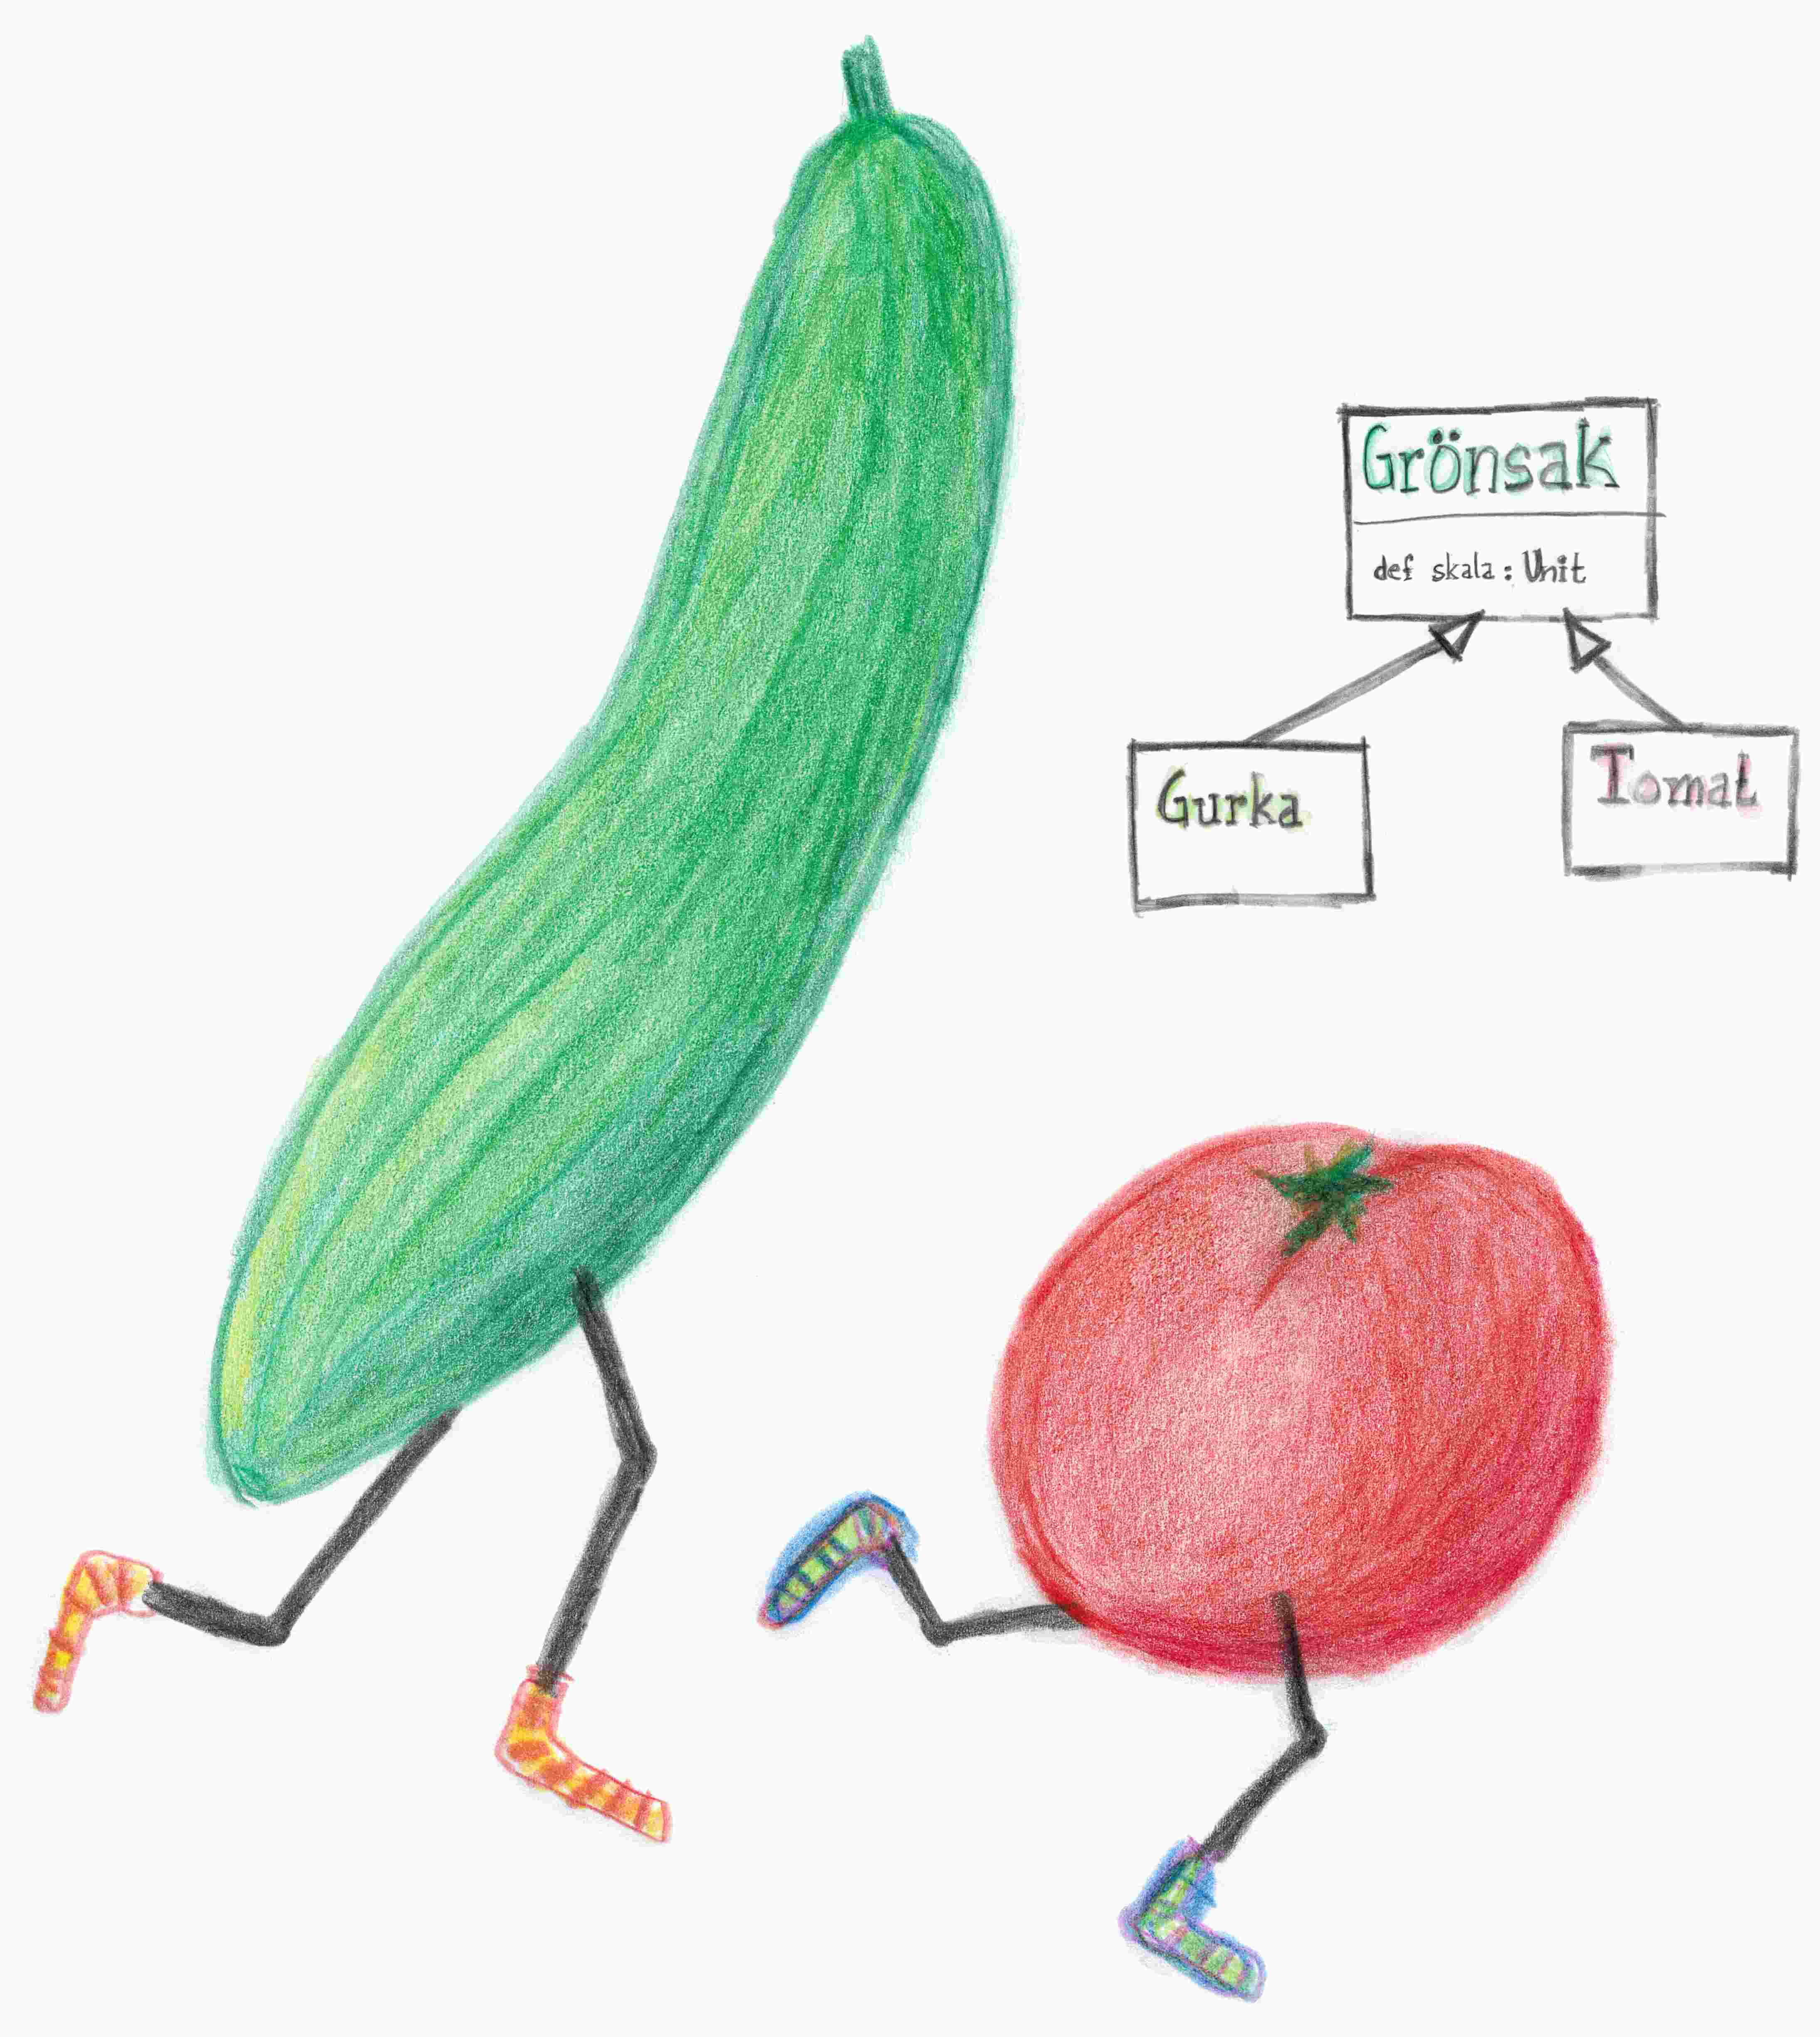
\includegraphics[height=12cm]{cover/gurka.jpg}
}

%\author{Redaktör: Björn Regnell}
\date{\raggedbottom%
\vspace{-2em}\begin{minipage}{1.0\textwidth}\centering
EDAA45, Lp1-2, HT 2016\\ 
Datavetenskap, LTH\\ 
Lunds Universitet\\
~\\
Kompileringsdatum: \today \\
\url{http://cs.lth.se/pgk} 
\end{minipage}
}

\usepackage{pgffor}  %% http://stackoverflow.com/questions/2561791/iteration-in-latex
                     %  allows:  \foreach \n in {1,...,4}{ do something with \n }

\usepackage{framed}  %  allows:   \begin{framed}\end{framed}
%\newenvironment{Slide}[2][]
%  {\begin{framed}\setlist{noitemsep}\section*{#2}}
%  {\end{framed}}

\newcommand{\SlideHeading}[1]{\section*{#1}}

\usepackage[most]{tcolorbox}
\newenvironment{Slide}[2][]
  {\vspace{0.5em}\begin{tcolorbox}[%width=1.05\textwidth,
  grow to right by=0.03\textwidth,grow to left by=0.03\textwidth,%breakable, 
                                   enhanced]\setlist{noitemsep}\SlideHeading{#2}}
  {\end{tcolorbox}\vspace{0.5em}}

\newcommand{\Subsection}[1]{} %ignore slide sections
\newcommand{\SlideOnly}[1]{} %ignore slide font size

\newif\ifkompendium  % to allow conditional text in slides only showing up in compendium
\kompendiumtrue      % in slides: \kompendiumfalse
                

%!TEX encoding = UTF-8 Unicode
\newcommand{\ExeWeekONE}{expressions}
\newcommand{\LabWeekONE}{kojo}

\newcommand{\ExeWeekTWO}{programs}
\newcommand{\LabWeekTWO}{--}

\newcommand{\ExeWeekTHREE}{functions}
\newcommand{\LabWeekTHREE}{blockmole}

\newcommand{\ExeWeekFOUR}{data}
\newcommand{\LabWeekFOUR}{pirates}

\newcommand{\ExeWeekFIVE}{sequences}
\newcommand{\LabWeekFIVE}{shuffle}

\newcommand{\ExeWeekSIX}{classes}
\newcommand{\LabWeekSIX}{turtlegraphics}

\newcommand{\ExeWeekSEVEN}{traits}
\newcommand{\LabWeekSEVEN}{turtlerace-team}

\newcommand{\ExeWeekEIGHT}{matching}
\newcommand{\LabWeekEIGHT}{chords-team}

\newcommand{\ExeWeekNINE}{matrices}
\newcommand{\LabWeekNINE}{maze}

\newcommand{\ExeWeekTEN}{sorting}
\newcommand{\LabWeekTEN}{survey}

\newcommand{\ExeWeekELEVEN}{scalajava}
\newcommand{\LabWeekELEVEN}{lthopoly-team}

\newcommand{\ExeWeekTWELVE}{threads}
\newcommand{\LabWeekTWELVE}{life}

\newcommand{\ExeWeekTHIRTEEN}{Uppsamling}
\newcommand{\LabWeekTHIRTEEN}{Projekt}

\newcommand{\ExeWeekFOURTEEN}{Extenta}
\newcommand{\LabWeekFOURTEEN}{--}


\begin{document}

\pagenumbering{roman}

\frontmatter
\maketitle
%!TEX encoding = UTF-8 Unicode
%!TEX root = ../compendium.tex

\clearpage\null\thispagestyle{empty}
\vfill

{
\setlength{\parindent}{0pt}
\emph{Editor}: Björn Regnell \\ 

%  LIST OF CONTRIBUTORS to https://github.com/lunduniversity/introprog
%    Please contact bjorn.regnell@cs.lth.se if you think you should be 
%    on this list, or make a pull request with an update of file briefly 
%    describing your contribtion in the commit text. 
%    This work is licenced under CC-BY-SA-4.0.
%!TEX encoding = UTF-8 Unicode
%!TEX root = compendium/compendium.tex
\hyphenation{Borg-lund Da-ne-bjer Grampp Palm-qvist Ravn-borg Ro-sen-qvist Schrei-ter Wih-lan-der}
\emph{Contributors} in alphabetical order:
Anders Buhl,
Anna Axelsson,
Anna Palmqvist Sjövall,
Anton Andersson,
Björn Regnell,
Casper Schreiter,
Cecilia Lindskog,
David Söderberg,
Emelie Engström,
Emil Wihlander,
Erik Bjäreholt,
Erik Grampp,
Fredrik Danebjer,
Gustav Cedersjö,
Henrik Olsson,
Jakob Hök,
Johan Ravnborg,
Jonas Danebjer,
Jos Rosenqvist,
Måns Magnusson,
Maj Stenmark,
Oscar Sigurdsson,
Oskar Berg,
Oskar Widmark,
Patrik Persson,
Per Holm,
Sandra Nilsson,
Sebastian Hegardt,
Simon Persson,
Stefan Jonsson,
Tim Borglund,
Tom Postema,
Valthor Halldorsson, 
Viktor Claesson.

\\ \newline

\emph{Home}: \url{https://cs.lth.se/pgk} \newline

\emph{Repo}: \url{https://github.com/lunduniversity/introprog} \\ \newline

This compendium is on-going work. \\ \textbf{Contributions are welcome!} \\ 
\emph{Contact}: \url{bjorn.regnell@cs.lth.se}
\\ \newline

\emph{Cover art}: Björn Regnell (inspired by Poul Ströyer's illustration of Lennart Hellsing's lyrics to  the childrens song ''Herr Gurka'' with music by Knut Brodin)\\ \newline

~\\ \newline

\emph{LICENCE}: CC BY-SA 4.0 \\
\url{http://creativecommons.org/licenses/by-sa/4.0/} \\
Please do \emph{not} distribute your solutions to lab assignments and projects. 
\\ \newline
Copyright \copyright~ 2015-2016. \\
Dept. of Computer Science, LTH, Lund University. Lund. Sweden.\\
}
%!TEX encoding = UTF-8 Unicode
%!TEX root = ../compendium.tex

\ChapterUnnum{Framstegsprotokoll}\label{progress-protocoll} 


\subsubsection*{Genomförda övningar}

\vspace{1em}\noindent 
{Till varje laboration hör en övning med uppgifter som utgör förberedelse inför labben. Du behöver minst behärska grunduppgifterna för att klara labben inom rimlig tid. Om du känner att du behöver öva mer på grunderna, gör då även extrauppgifterna. Om du vill fördjupa dig, gör fördjupningsuppgifterna som är på mer avancerad nivå. Kryssa för nedan vilka övningar du har gjort, så blir det lättare för din handledare att anpassa dialogen till de kunskaper du förvärvat hittills.}

\newcommand{\TickBox}{\raisebox{-.50ex}{\Large$\square$}}
\newcommand{\ExeRow}[1]{\hyperref[section:exe:#1]{\texttt{#1}} & \TickBox  &  \TickBox &  \TickBox  \\ \addlinespace }

\begin{table}[h]
\centering
\vspace{2em}
\begin{tabular}{lccc}
\toprule \addlinespace 
{\sffamily\small Övning} & 
{\sffamily\small Grund} &	
{\sffamily\small Extra} &
{\sffamily\small Fördjupning}\\ \addlinespace \midrule \\[-0.7em]
%!TEX encoding = UTF-8 Unicode
\ExeRow{expressions}
\ExeRow{programs}
\ExeRow{functions}
\ExeRow{data}
\ExeRow{sequences}
\ExeRow{classes}
\ExeRow{traits}
\ExeRow{matching}
\ExeRow{matrices}
\ExeRow{sorting}
\ExeRow{scalajava}
\ExeRow{threads}
\bottomrule
\end{tabular}
\end{table}

\newpage

\subsubsection*{Godkända obligatoriska moment}

\vspace{1em}\noindent 
För att bli godkänd på laborationsuppgifterna och projektuppgiften måste du lösa deluppgifterna och diskutera dina lösningar med en handledare. Denna diskussion är din möjlighet att få feedback på dina lösningar. Ta vara på den!
Se till att handledaren noterar nedan när du blivit godkänd på respektive labb. Spara detta blad tills du fått slutbetyg i kursen. 


\vspace{2.5em}\noindent Namn: \dotfill\\

\vspace{1em}\noindent Namnteckning: \dotfill\\

\newcommand{\LabRow}[1]{\\[-1.1em] \hyperref[section:lab:#1]{\texttt{#1}} & \dotfill &  \dotfill  \\ \addlinespace }

\begin{table}[h]
\centering
\vspace{1em}
\begin{tabular}{lcc}
\toprule \addlinespace 
{\sffamily\bfseries\small Lab} & {\sffamily\small Datum gk} &	{\sffamily\small Handledares namnteckning}\\ \addlinespace \midrule \\[-0.5em]
%!TEX encoding = UTF-8 Unicode
\LabRow{kojo}
\LabRow{blockmole}
\LabRow{pirates}
\LabRow{shuffle}
\LabRow{turtlegraphics}
\LabRow{turtlerace-team}
\LabRow{chords-team}
\LabRow{maze}
\LabRow{surveydata}
\LabRow{lthopoly-team}
\LabRow{life}
\LabRow{Projekt}
%\toprule 
\addlinespace \midrule \addlinespace
{\sffamily\small {\bfseries Projektuppgift} (välj en)	} & 
\multicolumn{2}{c}{\textit{Om egendef., ge kort beskrivning:}}  \\ 
\addlinespace\addlinespace %\midrule
{\Large$\square$}\texttt{~~~\hyperref[section:proj:bank]{bank}}  &  &  \\
{\Large$\square$}\texttt{~~~\hyperref[section:proj:imageprocessing]{imageprocessing}}  \\
{\Large$\square$}\texttt{~~~\hyperref[section:proj:tictactoe]{tictactoe}} \\  
{\Large$\square$}\texttt{~~~}\textit{egendefinerad}  \\
\\
\\
%\dotfill  \\
\bottomrule
\end{tabular}
\end{table}
%!TEX encoding = UTF-8 Unicode
%!TEX root = ../compendium.tex


\ChapterUnnum{Förord} 

Programmering är inte bara ett sätt att ta makten över de människoskapade system som är förutsättningen för vårt moderna samhälle. Programmering är också ett kraftfullt verktyg för tanken. Med kunskap i programmeringens grunder kan du påbörja den livslånga läranderesa som det innebär att vara systemutvecklare och abstraktionskonstnär. Programmeringsspråk och utvecklingsverktyg kommer och går, men de grundläggande koncepten bakom \emph{all} mjukvara består: sekvens, alternativ, repetition och abstraktion. 

Detta kompendium utgör kursmaterial för en grundkurs i programmering, som syftar till att ge en solid bas för ingenjörsstudenter och andra som vill utveckla system med mjukvara. Materialet omfattar en termins studier på kvartsfart och förutsätter kunskaper motsvarande gymnasienivå i svenska, matematik och engelska. 

Kompendiet är framtaget för och av studenter och lärare, och distribueras som öppen källkod. Det får användas fritt så länge erkännande ges och eventuella ändringar publiceras under samma licens som ursprungsmaterialet. På kurshemsidan \href{http://cs.lth.se/pgk}{cs.lth.se/pgk} och i kursrepot \href{http://github.com/lunduniversity/introprog}{github.com/lunduniversity/introprog} finns instruktioner om hur du kan bidra till kursmaterialet.

Läromaterialet fokuserar på lärande genom praktiskt programmeringsarbete och innehåller övningar och laborationer som är organiserade i moduler. Varje modul har ett tema och en teoridel som bearbetas på föreläsningar. 

I kursen använder vi språken Scala och Java för att illustrera grunderna i imperativ och objektorienterad programmering, tillsammans med elementär funktionsprogrammering. Mer avancerad objektorientering och funktionsprogrammering lämnas till efterföljande fördjupningskurser. 

Den kanske viktigaste framgångsfaktorn vid studier i programmering är att du bejakar din egen upptäckarglädje och experimentlusta. Det fantastiska med programmering är att dina egna intellektuella konstruktioner faktiskt \emph{gör} något som just \emph{du} har bestämt! Ta vara på det och prova dig fram genom att koda egna idéer -- det är kul när det funkar, men minst lika lärorikt är felsökning, buggrättande och alla misslyckade försök som, ibland efter hårt arbete vänds till lyckade lösningar och/eller bestående lärdomar. 

Välkommen i datavetenskapens fascinerande värld och hjärtligt lycka till med dina studier!

\vspace{1em}\noindent \textit{\hfill Lund, \today, Björn Regnell}





\setcounter{tocdepth}{2} % set headings level in table of contents
\tableofcontents
\mainmatter

\pagenumbering{arabic}

\part{Om kursen}      
%!TEX encoding = UTF-8 Unicode
%!TEX root = ../compendium.tex

\ChapterUnnum{Kursens arkitektur}

%!TEX encoding = UTF-8 Unicode
%!TEX root = ../lect-week01.tex

%%%%%%%%%%%%%%%%%%%%%%%%%%%%%%%%%%%%%%
\Subsection{Om kursen}

%%%

\ifkompendium\else
\begin{Slide}{Nytt för i år}
\begin{itemize}
\item \Emph{Scala} införs som förstaspråk på Datateknikprogrammet.
\item Den \Emph{största förnyelsen} av den inledande programmeringskursen sedan vi införde Java 1997.
\item Allt kursmaterial är \Emph{öppen källkod}.
\item \Emph{Studentermedverkan} i kursutvecklingen.
\end{itemize}
\vspace{1em}\hskip1em\href{https://www.lth.se/nyheter-och-press/nyheter/visa-nyhet/article/scala-blir-foerstaspraak-paa-datateknikprogrammet/}{www.lth.se/nyheter-och-press/nyheter/visa-nyhet/article/\\\hskip1emscala-blir-foerstaspraak-paa-datateknikprogrammet/}
\end{Slide}
\fi

\begin{Slide}{Veckoöversikt}
\noindent\resizebox{0.9\columnwidth}{!}{
%!TEX encoding = UTF-8 Unicode
\begin{tabular}{l|l|l|l}
\textit{W} & \textit{Modul} & \textit{Övn} & \textit{Lab} \\ \hline \hline
W01 & Introduktion            & expressions & kojo            \\
W02 & Kodstrukturer           & programs    & --              \\
W03 & Funktioner, Objekt      & functions   & simplewindow    \\
W04 & Datastrukturer          & data        & textfiles       \\
W05 & Sekvensalgoritmer       & sequences   & cardgame        \\
W06 & Klasser, Likhet         & classes     & shapes          \\
W07 & Arv, Gränssnitt         & traits      & turtlerace-team \\
KS  & KONTROLLSKRIVN.         & --          & --              \\
W08 & Mönster, Undantag       & matching    & chords-team     \\
W09 & Matriser, Typparametrar & matrices    & maze            \\
W10 & Sökning, Sortering      & sorting     & surveydata-team \\
W11 & Scala och Java          & scalajava   & scalajava-team  \\
W12 & Trådar                  & threads     & life            \\
W13 & Design                  & Uppsamling  & Inl.Uppg.       \\
W14 & Tentaträning            & Extenta     & --              \\
T   & TENTAMEN                & --          & --              \\
\end{tabular}

}
\end{Slide}

\ifkompendium
\noindent Kursen består av en \textbf{modul} per läsvecka med två \textbf{föreläsningar}, en \textbf{övning} och en \textbf{laboration} (undantaget W02, W13 \& W14 som saknar labb och/eller övning). 
Föreläsningarna ger en översikt av den teori som ingår i varje modul. Genom att göra övningarna bearbetar du teorin och förebereder dig inför laborationerna. När du klarat övningen och laborationen i en modul är du redo att gå vidare till nästa. Tabellen på nästa uppslag visar begrepp som ingår i varje modul. 

Kursen är uppdelad i två läsperioder. Efter första läsperioden gör du en diagnostisk \textbf{kontrollskrivning} som kontrollerar ditt kunskapsläge. Andra läsperioden avslutas med ett större \textbf{projekt} och en skriftlig \textbf{tentamen}.



\clearpage
\hyphenation{intro-duktion sekvens-algoritmer kod-strukturer data-strukturer}
{\fontsize{11}{13}\selectfont\renewcommand{\arraystretch}{1.75}
\begin{longtable}{@{}p{.05\textwidth} | >{\hspace{0.1em}\raggedright\bfseries\sffamily}p{.15\textwidth}  >{\raggedleft\arraybackslash\hspace{0.0em}\fontsize{10.5}{12}\selectfont}p{0.735\textwidth}}
W01 & Introduktion & sekvens, alternativ, repetition, abstraktion, programmeringsspråk, programmeringsparadigmer, editera-kompilera-exekvera, datorns delar, virtuell maskin, REPL, literal, värde, uttryck, identifierare, variabel, typ, tilldelning, namn, val, var, def, inbyggda grundtyper, Int, Long, Short, Double, Float, Byte, Char, String, println, typen Unit, enhetsvärdet (), stränginterpolatorn s, if, else, true, false, MinValue, MaxValue, aritmetik, slumptal, math.random, logiska uttryck, de Morgans lagar, while-sats, for-sats \\
W02 & Kodstrukturer & iterering, for-uttryck, map, foreach, Range, Array, Vector, algoritm vs implementation, pseudokod, algoritm: SWAP, algoritm: SUM, algoritm: MIN/MAX, algoritm: MININDEX, block, namnsynlighet, namnöverskuggning, lokala variabler, paket, import, filstruktur, jar, dokumentation, programlayout, JDK, main i Java vs Scala, java.lang.System.out.println \\
W03 & Funktioner, objekt & definera funktion, anropa funktion, parameter, returtyp, värdeandrop, namnanrop, default-argument, namngivna argument, applicera funktion på alla element i en samling, procedur, värdeanrop vs namnanrop, uppdelad parameterlista, skapa egen kontrollstruktur, objekt, modul, punktnotation, tillstånd, metod, medlem, funktionsvärde, funktionstyp, äkta funktion, stegad funktion, apply, lazy val, lokala funktioner, anonyma funktioner, lambda, aktiveringspost, anropsstacken, objektheapen, rekursion  cslib.window.SimpleWindow \\
W04 & Datastrukturer & attribut (fält), medlem, metod, tupel, klass, Any, isInstanceOf, toString, case-klass, samling, scala.collection, föränderlighet vs oföränderlighet, List, Vector, Set, Map, typparameter, generisk samling som parameter, översikt samlingsmetoder, översikt strängmetoder, läsa/skriva textfiler, Source.fromFile, java.nio.file \\
W05 & Sekvensalgoritmer & sekvensalgoritm, algoritm: SEQ-COPY, in-place vs copy, algoritm: SEQ-REVERSE, algoritm: SEQ-REGISTER, sekvenser i Java vs Scala, for-sats i Java, java.util.Scanner, scala.collection.mutable.ArrayBuffer, StringBuilder, java.util.Random, slumptalsfrö \\
W06 & Klasser & objektorientering, klass, Point, Square, Complex, new, null, this, inkapsling, accessregler, private, private[this], kompanjonsobjekt, getters och setters, klassparameter, primär konstruktor, objektfabriksmetod, överlagring av metoder, referenslikhet vs strukturlikhet, eq vs == \\
W07 & Arv & arv, polymorfism, trait, extends, asInstanceOf, with, inmixning, supertyp, subtyp, bastyp, override, klasshierarkin i Scala: Any AnyRef Object AnyVal Null Nothing, referenstyper vs värdetyper, klasshierarkin i scala.collection, Shape som bastyp till Rectangle och Circle, accessregler vid arv, protected, final, klass vs trait, abstract class, case-object, typer med uppräknade värden \\
KS & \multicolumn{2}{l}{KONTROLLSKRIVN.} \\
W08 & Repetition, trösklar, luckor & REBOOT CAMP: identifiera dina egna lärandetrösklar och kunskapsluckor, kom-i-kapp med övningar och labbar, repetera, fördjupning för de som är redo, specialträning för behövande \\
W09 & Mönster, undantag & mönstermatchning, match, Option, throw, try, catch, Try, unapply, sealed, flatten, flatMap, partiella funktioner, collect, speciella matchningar: wildcard pattern; variable binding; sequence wildcard; back-ticks, equals, hashcode, exempel: equals för klassen Complex, switch-sats i Java \\
W10 & Matriser, typparametrar & matris, nästlad samling, nästlad for-sats, typparameter, generisk funktion, generisk klass, fri vs bunden typparameter, matriser i Java vs Scala, allokering av nästlade arrayer i Scala och Java \\
W11 & Sökning, sortering & strängjämförelse, compareTo, implicit ordning, linjärsökning, binärsökning, algoritm: LINEAR-SEARCH, algoritm: BINARY-SEARCH, algoritmisk komplexitet, sortering till ny vektor, sortering på plats, insättningssortering, urvalssortering, algoritm: INSERTION-SORT, algoritm: SELECTION-SORT, Ordering[T], Ordered[T], Comparator[T], Comparable[T] \\
W12 & Scala och Java & syntaxskillnader mellan Scala och Java, klasser i Scala vs Java, referensvariabler vs enkla värden i Java, referenstilldelning vs värdetilldelning i Java, alternativ konstruktor i Scala och Java, for-sats i Java, for-each-sats i Java, java.util.ArrayList, autoboxing i Java, primitiva typer i Java, wrapperklasser i Java, samlingar i Java vs Scala, scala.collection.JavaConverters, namnkonventioner för konstanter \\
W13 & Extra: design, api, trådar, webb & utvecklingsprocessen, krav-design-implementation-test, gränssnitt, trait vs interface, programmeringsgränssnitt (api), designexempel, tråd, jämlöpande exekvering, icke-blockerande anrop, callback, java.lang.Thread, java.util.concurrent.atomic.AtomicInteger, scala.concurrent.Future, kort om html+css+javascript+scala.js och webbprogrammering \\
W14 & \multicolumn{2}{l}{Tentaträning} \\
T & \multicolumn{2}{l}{TENTAMEN} \\
\end{longtable}
}
\fi

\begin{Slide}{Vad lär du dig?}
\begin{itemize}
\item Grundläggande principer för programmering:\\ Sekvens, Alternativ, Repetition, Abstraktion (SARA)\\$\implies$Inga förkunskaper i programmering krävs!
\item Konstruktion av algoritmer
\item Tänka i abstraktioner
\item Förståelse för flera olika angreppssätt: 
\begin{itemize}
\item \Emph{imperativ programmering}%: satser, föränderlighet
\item \Emph{objektorientering}%: inkapsling, återanvändning
\item \Emph{funktionsprogrammering}%: uttryck, oföränderlighet
\end{itemize}
\item Programspråken \Emph{Scala} och \Emph{Java}
\item Utvecklingsverktyg (editor, kompilator, utvecklingsmiljö)
\item Implementera, testa, felsöka
\end{itemize}
\end{Slide}

\begin{Slide}{Hur lär du dig?}
\begin{itemize}
\item Genom praktiskt \Alert{eget arbete}: \Emph{Lära genom att göra!}
\begin{itemize}
\item Övningar: applicera koncept på olika sätt
\item Laborationer: kombinera flera koncept till en helhet
\end{itemize}
\item Genom studier av kursens teori: \Emph{Skapa förståelse!}
\item Genom samarbete med dina kurskamrater: \Emph{Gå djupare!}
\end{itemize}
\end{Slide}


\begin{Slide}{Kurslitteratur}
\begin{minipage}{0.45\textwidth}\SlideFontSmall
\hskip1.33em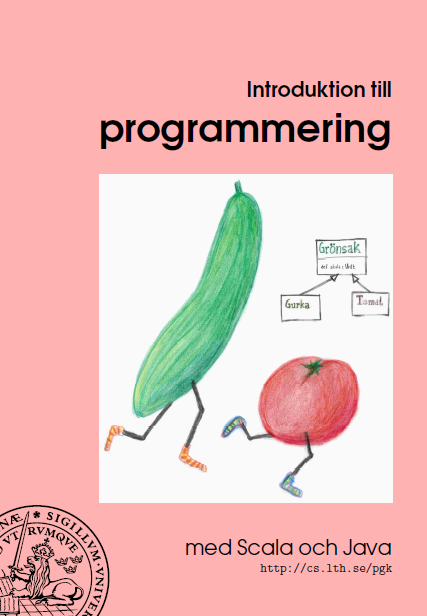
\includegraphics[width=0.65\textwidth]{../img/compendium-front-page.png}
\begin{itemize}
\item \Emph{Kompendium} med teori, övningar \& laborationer
\item Trycks \& säljs av institutionen %på KFS \\ \url{http://www.kfsab.se/}
 efter beställning
\end{itemize}
\end{minipage}
\hskip1em\begin{minipage}{0.5\textwidth}\SlideFontSize{8}{10}
\Emph{Rekommenderade böcker}; bra men ej nödvändig bredvidläsning om du vill ha bok:\\ 
-- för \Emph{nybörjare}:
\vskip0.2mm
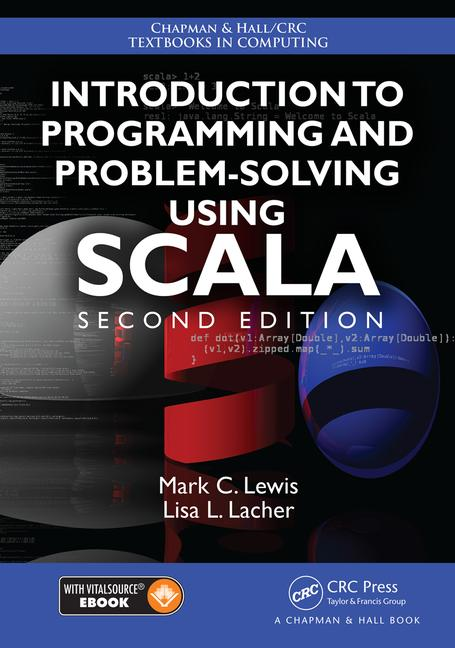
\includegraphics[width=0.33\textwidth]{../img/lewisbook.jpg}\hskip4mm
\includegraphics[width=0.33\textwidth]{../img/ankbok.jpg}

\noindent -- för de som \Emph{redan kodat} en del:
\vskip0.7mm
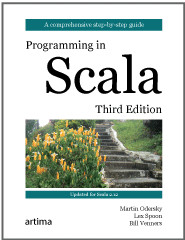
\includegraphics[width=0.45\textwidth]{../img/pinsbook.jpg}\hskip4mm
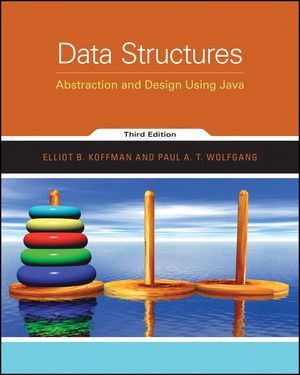
\includegraphics[width=0.47\textwidth]{../img/koffmanbook.jpg}
\end{minipage}
\end{Slide}

\ifkompendium\else
\begin{Slide}{Beställning av kompendium och snabbreferens}
\begin{itemize}
\item \Emph{Kompendiet} finns i pdf för fri nedladdning, men det \Alert{rekommenderas starkt} att du köper en tryckt variant.
\item Det är mycket lättare att ha övningar och labbar på papper bredvid skärmen, när du ska tänka, koda och plugga!
\item \Emph{Snabbreferensen} finns också i pdf men du behöver ha en tryckt version eftersom det är enda tillåtna hjälpmedlet på skriftliga kontrollskrivningen och tentamen.
\item Kompendium och bok trycks här i E-huset och säljs av institutionen till självkostnadspris.
\item Pris för kompendium + snabbreferens: ??? kr
\item Skriv upp dig på listan -- tryckning sker efter beställning.
\item Du betalar med jämna pengar på cs expedition, våning 2
\end{itemize}
\end{Slide}
\fi

\ifkompendium\else
\begin{Slide}{Personal}\SlideFontSmall
\begin{description}
\item [\bfseries Kursansvarig:] ~\\Björn Regnell, bjorn.regnell@cs.lth.se
\item [\bfseries Kurssekreterare:]  ~\\Lena Ohlsson \\Exp.tid 09.30 -- 11.30 samt 12.45 -- 13.30
\item [\bfseries Handledare:] ~\\
\Emph{Doktorander}: \\ 
Tekn. Lic. Maj Stenmark, Gustav Cedersjö\\
\Emph{Teknologer}: \\
Anders Buhl, 
Anna Palmqvist Sjövall, 
Anton Andersson,
Cecilia Lindskog, 
Emil Wihlander, 
Erik Bjäreholt, 
Erik Grampp, 
Filip Stjernström, 
Fredrik Danebjer, 
Henrik Olsson, 
Jakob Hök, 
Jonas Danebjer, 
Måns Magnusson, 
Oscar Sigurdsson, 
Oskar Berg, 
Oskar Widmark, 
Sebastian Hegardt, 
Stefan Jonsson, 
Tom Postema, 
Valthor Halldorsson
\end{description}
\end{Slide}
\fi

\begin{Slide}{Föreläsningsanteckningar}
\begin{itemize}
\item Föreläsningsanteckningar utvecklas under kursens gång
\item Några av bilderna finns i kompendiet
\item Alla bilder läggs ut här: \\
\href{https://github.com/lunduniversity/introprog/tree/master/slides}{github.com/lunduniversity/introprog/tree/master/slides} \\
och uppdateras kontinuerligt allt eftersom de utvecklas
\item Förslag på förbättringar välkomna!
\end{itemize}
\end{Slide}

\begin{Slide}{Kursmoment --- varför?}\SlideOnly{\footnotesize}
\begin{itemize}
\item \Emph{Föreläsningar}: skapa översikt, ge struktur, förklara teori, svara på frågor, motivera varför
\item \Emph{Övningar}: \Alert{förbereda} laborationerna, bearbeta teorins olika delar med avgränsade deluppgifter, \Emph{grundövningar} för alla, \Emph{extraövningar} om du vill/behöver öva mer, \Emph{fördjupningsövningar} om du vill gå djupare 
\item \Emph{Laborationer}: \Alert{obligatoriska}, sätta samman teorins delar i ett större program; lösningar redovisas för handledare; gk på alla för att få tenta, 
\item \Emph{Resurstider}: få hjälp med övningar och laborationsförberedelser av handledare, fråga vad du vill
\item \Emph{Samarbetsgrupper}: grupplärande genom samarbete, hjälpa varandra 
\item \Emph{Kontrollskrivning}: \Alert{obligatorisk}, diagnostisk, kamraträttad; kan ge samarbetsbonuspoäng till tentan
\item \Emph{Individuell projektuppgift}: \Alert{obligatorisk}, du visar att du kan skapa ett större program självständigt; redovisas för handledare
\item \Emph{Tentamen}: \Alert{obligatorisk}, skriftlig, enda hjälpmedel:   \href{https://github.com/lunduniversity/introprog/blob/master/quickref/quickref.pdf}{snabbreferensen}
\end{itemize}
\end{Slide}

\ifkompendium\else
\begin{Slide}{Detta är bara början... }
Exempel på efterföljande kurser som bygger vidare på denna:
\begin{itemize}
\item Årskurs 1
\begin{itemize}
\item Programmeringsteknik -- fördjupningskurs
\item Utvärdering av programvarusystem
\item Diskreta strukturer
\end{itemize}
\item Årskurs 2
\begin{itemize}
\item Objektorienterad modellering och design
\item Programvaruutveckling i grupp
\item Algoritmer, datastrukturer och komplexitet
\item Funktionsprogrammering
\end{itemize}
\end{itemize}
\end{Slide}


\begin{Slide}{Registrering}
\begin{itemize}
\item Fyll i listan som skickas runt.
\item Kryssa i kolumnen \Emph{Ska gå} om du ska gå kursen\footnote{\scriptsize D1:a som redan gått motsvarande högskolekurs? Uppsök studievägledningen}\footnote{\scriptsize D2:a eller äldre som vill bli omregistrerad? Prata med kursansvarig på rasten}
\item Kryssa i kolumnen \Emph{Kursombud} om du kan tänka dig att vara kursombud under kursens gång
\begin{itemize}
\item Alla LTH-kurser ska utvärderas under kursens gång och efter kursens slut.
\item Till det behövs kursombud -- ungefär 2 D-are och 2 W-are.
\item Ni kommer att bli kontaktade av studierådet. \\SRD ordf: Amelia Andersson
\end{itemize}
\end{itemize}
\end{Slide}

%%%
\begin{Slide}{Förkunskaper}
\begin{itemize}
\item Förkunskaper $\neq$ Förmåga
\item Varken kompetens eller personliga egenskaper är statiska 
\item ''Programmeringskompetens'' är inte \textit{en} enda enkel förmåga utan en komplex sammansättning av flera olika förmågor som utvecklas genom hela livet
\item Ett innovativt utvecklar\Alert{team} behöver många olika kompetenser för att vara framgångsrikt
\end{itemize}
\end{Slide}

%%%
\begin{Slide}{Förkunskapsenkät}
\begin{itemize}
\item Om du inte redan gjort det: fyll i denna enkät \Alert{snarast}:\\
\url{http://cs.lth.se/pgk/presurvey} \\
\item Dina svar behandlas internt och all statistik anonymiseras.
\item Enkäten ligger till grund för randomiserad gruppindelning i samarbetsgrupper, så att det blir en spridning av förkunskaper inom gruppen.
\item Gruppindelnig publiceras här: \\ \url{http://cs.lth.se/pgk/grupper/}
\end{itemize}
\end{Slide}

\begin{Slide}{Samarbetgrupper}\footnotesize
\begin{itemize}
\item Ni delas in i \Emph{samarbetsgrupper} om ca 5 personer baserat på förkunskapsenkäten, så att olika förkunskapsnivåer sammanförs
\item Några av laborationerna är mer omfattande \Emph{grupplabbar} och kommer att göras i samarbetsgrupperna \\ \vspace{1em}
\item Kontrollskrivningen i halvtid kan ge \Emph{samarbetsbonus} (max 5p) som adderas till ordinarie tentans poäng (max 100p) med medelvärdet av gruppmedlemmarnas individuella kontrollskrivningspoäng 
\scriptsize \parbox{7cm}{Bonus $b$ för varje person i en grupp med $n$ medlemmar med $p_i$ poäng vardera på kontrollskrivningen:} 
 \hspace{5mm} $\displaystyle b = \sum\limits_{i=1}^n \frac{p_i}{n}$
\end{itemize}
\end{Slide}

\fi

%%%
\begin{Slide}{Varför studera i samarbetsgrupper?}

Huvudsyfte: \Emph{Bra lärande!}

\begin{itemize}
\item Pedagogisk forskning stödjer tesen att lärandet blir mer djupinriktat om det sker i utbyte med andra
\item Ett studiesammanhang med höga ambitioner och respektfull gemenskap gör att vi \Emph{når mycket längre}
\item Varför ska du som redan kan mycket aktivt dela med dig av dina kunskaper?
\begin{itemize}
\item Förstå bättre själv genom att förklara för andra
\item Träna din pedagogiska förmåga
\item Förbered dig för ditt kommande yrkesliv som mjukvaruutvecklare 
\end{itemize}
\end{itemize}
\end{Slide}

%%%

\ifkompendium\else
\begin{Slide}{Samarbetskontrakt}
Gör ett skriftligt \href{https://github.com/bjornregnell/lth-eda016-2015/blob/master/assignments/collaboration-contract.tex}{\bf samarbetskontrakt} med dessa och ev. andra punkter som ni också tycker bör ingå:
\begin{enumerate}
\item Återkommande mötestider per vecka
\item Kom i tid till gruppmöten
\item Var väl förberedd genom självstudier inför gruppmöten
\item Hjälp varandra att förstå, men ta inte över och lös allt
\item Ha ett respektfullt bemötande även om ni har olika åsikter
\item Inkludera alla i gemenskapen
\end{enumerate}

Diskutera hur ni ska uppfylla dessa innan alla skriver på. \\ Ta med samarbetskontraktet och visa för handledare på labb 1.

\vskip1em

\Alert{Om arbetet i samarbetsgruppen inte fungerar ska ni mejla kursansvarig och boka mötestid!}
\end{Slide}

\begin{Slide}{Bestraffa inte frågor!}
\begin{itemize}
\item Det finns bättre och sämre frågor vad gäller hur mycket man kan lära sig av svaret, men \Emph{all undran är en chans} att i dialog utbyta erfarenheter och lärande
\item Den som frågar \Emph{vill veta} och berättar genom frågan något om nuvarande kunskapsläge
\item Den som svarar får chansen att \Emph{reflektera} över vad som kan vara svårt och olika vägar till djupare förståelse
\item I en hälsosam lärandemiljö är det \Emph{helt tryggt} att visa att man ännu inte förstår, att man gjort ''fel'', att man har mer att lära, etc. 
\item Det är viktigt att våga försöka även om det blir ''fel'':\\ \Emph{det är ju då man lär sig!}
\end{itemize}
\end{Slide}

%%%
\begin{Slide}{Plagiatregler}
Läs dessa regler noga och diskutera i samarbetsgrupperna:
\begin{itemize}
\footnotesize
\item \url{http://cs.lth.se/utbildning/samarbete-eller-fusk/}
\item \url{http://cs.lth.se/utbildning/foereskrifter-angaaende-obligatoriska-moment/}
\end{itemize}
Ni ska lära er genom \Emph{eget arbete} och genom  \Emph{bra samarbete}. Samarbete gör att man lär sig bättre, men man lär sig inte av att bara kopiera andras lösningar. Plagiering är förbjuden och kan medföra disciplinärende och avstängning.
\end{Slide}

\fi %%%%%%%%%%%%%%%%%%%%%%%%%%%%%%%%

%%%
\begin{Slide}{En typisk kursvecka}
\begin{enumerate}
\item Gå på \Emph{föreläsningar} på \Alert{måndag--tisdag}
\item Jobba med \Emph{individuellt} med teori, övningar, labbförberedelser på  \Alert{måndag--torsdag}
\item Kom till \Emph{resurstiderna} och få hjälp och tips av handledare och kurskamrater på \Alert{onsdag--torsdag}
\item Genomför den obligatoriska \Emph{laborationen} på \Alert{fredag}
\item Träffas i \Emph{samarbetsgruppen} och hjälp varandra att förstå mer och fördjupa lärandet, förslagsvis på återkommande tider varje vecka då alla i gruppen kan
\end{enumerate}
Se detaljerna och undantagen i schemat: \href{http://cs.lth.se/pgk/schema}{cs.lth.se/pgk/schema}
\end{Slide}

\ifkompendium\else  %%%%%%%%%%%%%%%%%%%%%%%%%
%%%
\begin{Slide}{Laborationer}\footnotesize
\begin{itemize}
\item \Alert{Programmering lär man sig bäst genom att programmera...}
\item Labbarna är \Emph{individuella} (utom 2) och \Emph{obligatoriska}
\item Gör övningarna och labbförberedelserna noga \textit{innan} själva labben -- detta är ofta helt nödvändigt för att du ska hinna klart. Dina labbförberedelserna kontrolleras av handledare under labben.
\item Är du sjuk? Anmäl det \Alert{före} labben till \url{bjorn.regnell@cs.lth.se}, \\ få hjälp på resurstid och redovisa på resurstid (eller labbtid, när handledaren har tid över)
\item Hinner du inte med hela? Se till att handledaren noterar din närvaro, och fortsätt på resurstid och ev. uppsamlingstider.
\item Läs noga anvisningarna i kompendiet
\item Laborationstiderna är gruppindelade enligt \href{http://cs.lth.se/eda016/schema/}{schemat}. Du ska gå till den tid och den sal som motsvarar din \href{http://cs.lth.se/eda016/grupper/}{grupp}.
\end{itemize}
\end{Slide}

%%%
\begin{Slide}{Resurstider}
\begin{itemize}
\item På resurstiderna får du hjälp med övningar och laborationsförberedelser
\item Kom till minst en resurstid per vecka (se \href{http://cs.lth.se/eda016/schema/}{schema})
\item Handledare gör ibland \Emph{genomgångar} för alla under resurstiderna. Tipsa om handledare om vad du finner svårt.
\item Resurstiderna är inte gruppindelade i schemat. Du får i mån av plats gå på flera resurstider per vecka. Om det blir fullt i ett rum prioriteras dessa grupper för att minimera schemakrockar: 
\end{itemize}
\begin{table}[]
\centering\scriptsize
\begin{tabular}{lllll}
Tid Lp1 & Sal & Grupper med prio \\
\hline
Ons 10-12 v1-7 & Hacke  &   09 \& 10 \\
Ons 13-15 v1-7 & Hacke  &   07 \& 08  \\
Ons 15-17 v1-7 & Panter  & 05 \& 06   \\
Ons 15-17 v1-7 & Val       &  03 \& 04   \\
Tor 13-15 v1-7 & Mars     & 01 \& 02  \\
Tor 15-17 v1-7 & Mars     & 11 \& 12 \\ 
\end{tabular}
\end{table}
\end{Slide}

\fi
%!TEX encoding = UTF-8 Unicode
%!TEX root = ../compendium.tex

\chapter{Anvisningar}

Detta kapitel innehåller anvisningar och riktlinjer för kursens olika delar. Läs noga så att du inte missar viktig information om syftet bakom kursmomenten och vad som förväntas av dig.

\section{Samarbetsgrupper}

Ditt lärande i allmänhet, och ditt programmeringslärande i synnerhet, fördjupas om det sker i dialog med andra. Dessutom är din samarbetsförmåga och din pedagogiska förmåga avgörande för din framgång som professionell systemutvecklare. Därför är kursdeltagarna indelade i \emph{samarbetsgrupper} om 4-6 personer där medlemmarna samverkar för att alla i gruppen ska nå så långt som möjligt i sina studier.

För att hantera och dra nytta av skillnader i förkunskaper är samarbetsgrupperna indelade så att deltagarnas har \emph{varierande förkunskaper} baserat på en förkunskapsenkät. De som redan har provat på att programmera får då chansen att träna på sin pedagogiska förmåga som är så viktig för systemutvecklare, medan de som ännu inte kommit lika långt kan dra nytta av gruppmedlemmarnas samlade kompetens i sitt lärande. Kompetensvariationen i gruppen kommer att förändras under kursens gång, då olika individer lär sig olika snabbt i olika skeden av sitt lärande; de som till att börja med har ett försprång kanske senare får kämpa för att komma över en viss lärandetröskel.

Samarbetsgrupperna organiserar själva sitt arbete och varje grupp får finna de samarbetsformer som passar medlemmarna bäst. Här följer några erfarenhetsbaserade tips:

\begin{enumerate}
\item Träffas så fort som möjligt i hela gruppen och lär känna varandra. Ju snabbare ni kommer samman som grupp och får den sociala interaktionen att fungera desto bättre. Ni kommer att ha nytta av denna investering under hela terminen och kanske under resten av er studietid.
\item Kom överens om stående mötestider och mötesplatser. Det är viktigt med kontinuiteten i arbetet för att samarbetet i gruppen ska utvecklas och fördjupas. Träffas minst en gång i veckan. Ha en stående agenda, t.ex. en runda runt bordet där var och en berättar hur långt hen kommit och listar de begreppen som hen för tillfället behöver fokusera på.
\item Hjälps åt att tillsammans identifiera och diskutera era olika individuella studiebehov och studieambitioner. När man ska lära sig att programmera stöter man på olika lärandetrösklar som man kan få hjälp att ta sig över av någon som redan är förbi tröskeln. Men det gäller då för den som hjälper att först förstå exakt vad det är som är svårt, eller vilka specifika pusselbitar som saknas, för att på bästa sätt kunna underlätta för en medstudent att ta sig över tröskeln. Det gäller att hjälpa \emph{lagom} mycket så att var och en självständigt får chansen att skriva sin egen kod.
\item Var en schysst kamrat och agera professionellt, speciellt i situationer där gruppdeltagarna vill olika. Kommunicera på ett respektfullt sätt och sök konstruktiva kompromisser. Att utvecklas socialt är viktigt för din framtida yrkesutövning som systemutvecklare och i samarbetsgruppen kan du träna och utveckla din samarbetsförmåga.
\end{enumerate}

\subsection{Samarbetskontrakt}

Ni ska upprätta ett samarbetskontrakt redan under första veckan och visa för en handledare. Alla gruppmedlemmarna ska skriva under kontraktet. Handledaren ska också skriva under som bekräftelse på att ni visat kontraktet.

Syftet med kontraktet är att ni ska diskutera igenom i gruppen hur ni vill arbeta och vilka regler ni tycker är rimliga. Ni bestämmer själva vad kontraktet ska innehålla. Nedan finns förslag på punkter som kan ingå i ert kontrakt. En kontraktsmall finns här: \url{https://github.com/lunduniversity/introprog/blob/master/admin/collaboration-contract.tex}

\begin{tcolorbox}%[width=1.05\textwidth,  grow to right by=0.03\textwidth,grow to left by=0.03\textwidth,breakable, enhanced]
\subsubsection*{Samarbetskontrakt}
Vi som skrivit under detta kontrakt lovar att göra vårt bästa för att följa samarbetsreglerna nedan, så att alla ska lära sig så mycket som möjligt.
\begin{enumerate}
\item Komma i tid till gruppmöten.
\item Vara väl förberedda genom självstudier inför gruppmöten.
\item Hjälpa varandra att förstå, men inte ta över och lösa allt åt någon annan.
\item Ha ett respektfullt bemötande även om vi har olika åsikter.
\item Inkludera alla i gemenskapen.
\item ...
\end{enumerate}
\end{tcolorbox}
\subsection{Grupplaborationer}\label{subsection:grouplabs}



Det finns två typer av laborationer: individuella laborationer och grupplaborationer. Det flesta av kursens laborationer är individuella, medan laborationerna i veckorna W07, W08 och W11 genomförs av respektive samarbetsgrupp gemensamt. Följande anvisningar gäller speciellt för grupplaborationer. (Allmänna anvisningar för laborationer finns i avsnitt \ref{section:labs}.)

\begin{enumerate}
%!TEX encoding = UTF-8 Unicode
%!TEX root = compendium.tex
\item 
Diskutera i din samarbetsgrupp hur ni ska dela upp koden mellan er i flera olika delar, som ni kan arbeta med var för sig. En sådan del kan vara en klass, en trait, ett objekt, ett paket, eller en funktion. 
\item
Varje del ska ha en \emph{huvudansvarig} individ. 
\item
Arbetsfördelningen ska vara någorlunda jämt fördelad mellan gruppmedlemmarna.
\item
När ni redovisar er lösning ska ni börja med att redogöra för handledaren hur ni delat upp koden och vem som är huvudansvarig för vad. 
\item
Den som är huvudansvarig för en viss del redovisar den delen.
\item 
Grupplaborationer görs i huvudsak som hemuppgift. Salstiden används primärt för redovisning.
\end{enumerate}

\subsection{Samarbetsbonus}\label{section:bonus}

Alla tjänar på att samarbeta och hjälpa varandra i lärandet. Som extra incitament för grupplärande utdelas \emph{samarbetsbonus} baserat på resultatet från den diagnostiska kontrollskrivningen efter halva kursen (se avsnitt \ref{section:diagnostic-test}). Bonus ges till varje student enligt gruppmedelvärdet av kontrollskrivningspoängen och räknas ut med funktionen \code{collaborationBonus} nedan, där \code{points} är en sekvens med heltal som utgör gruppmedlemmars individuella poäng från kontrollskrivningen.

\begin{Code}
  def collaborationBonus(points: Seq[Int]): Int =
    (points.sum / points.size.toDouble).round.toInt
\end{Code}

Samarbetsbonusen viktas så att den högsta möjliga bonusen maximalt utgör $5\%$ av maxpoängen på tentan och adderas till det individuella tentaresultatet om du är godkänd på kursens sluttentamen. Samarbetsbonusen kan alltså påverka om du når högre betyg, men den påverkar \emph{inte} om du får godkänt eller ej. Detta gör att alla i gruppen gynnas av att så många som möjligt lär sig på djupet inför kontrollskrivningen. Din eventuella samarbetsbonusen räknas dig tillgodo endast vid det första, ordinarie tentamenstillfället.

\section{Föreläsningar}

En normal läsperiodsvecka börjar med två föreläsningspass om $2$ timmar vardera. Föreläsningarna ger en översikt av kursens teoretiska innehåll och går igenom innebörden av de begrepp du ska lära dig. Föreläsningarna innehåller många programmeringsexempel och föreläsaren ''lajvkodar'' då och då för att illustrera den kreativa problemlösningsprocess som ingår i all programmering. Föreläsningarna berör även kursens organisation och olika praktiska detaljer.

På föreläsningarna ges goda möjligheter att ställa allmänna frågor om teorin och att i plenum diskutera specifika svårigheter (individuell lärarhjälp ges på resurstider, se avsnitt \ref{section:tutorials}, och på laborationer, se avsnitt \ref{section:labs}). Även om det är många i föreläsningssalen, \emph{tveka inte att ställa frågor} -- det är säkert fler som undrar samma sak som du!

Föreläsningarna är inte obligatoriska, men det är mycket viktigt att du går dit, även om du i perioder känner att du har bra koll på all teori. På föreläsningarna får du en övergripande ämnesstruktur och en konkret programmeringsupplevelse, som du delar med dina kursare och kan diskutera i samarbetsgrupperna. Föreläsningarna ger också en prioritering av materialet och förbereder dig inför examinationen med praktiska råd och tips om hur du bör fokusera dina studier.

\section{Övningar}

I en normal läsperiodsvecka ingår en övning med flera uppgifter och deluppgifter.
Övningarna utgör basen för dina programmeringsstudier och erbjuder en systematisk genomgång av kursteorins alla delar genom praktiska kodexempel som du genomför steg för steg vid datorn med hjälp av ett interaktivt verktyg som kallas Read-Evaluate-Print-Loop (REPL). Om du gör övningarna i REPL säkerställer du att du skaffar dig tillräcklig förståelse för alla begrepp som ingår i kursen och att du inte missar någon viktigt pusselbit.

Övningarna utgör också förberedelse inför laborationerna. Om du inte gör veckans övning är det inte troligt att du kommer att klara veckans laboration inom rimlig tid.

Dessa två punkter är speciellt viktiga när du ska lära sig att programmera:
\begin{itemize}
\item \textbf{Programmera!} Det räcker inte med att bara passivt läsa om programmering; du måste \emph{aktivt} själv skriva mycket kod och genomföra egna programmeringsexperiment. Det underlättar stort om du bejakar din nyfikenhet och experimentlusta. Alla programmeringsfel som du gör och alla dina misstag, som i efterhand verkar enkla, är i själva verket oumbärliga steg på vägen och ger avgörande \emph{''Aha!''}-upplevelser. Kursens övningarna är grunden för denna form av lärande.

\item \textbf{Ha tålamod!} Det är först när du har förmågan att aktivt kombinera \emph{många} olika programmeringskoncept som du själv kan lösa lite större programmeringsuppgifter. Det kan vara frustrerande i början innan du når så långt att din verktygslåda med begrepp är tillräckligt stor för att du ska kunna skapa den kod du vill. Ibland krävs det extra tålamod innan allt plötslig lossnar. Många programmeringslärare och -studenter vittnar om att ''polletten plötsligt trillar ner'' och allt faller på plats. Övningarna syftar till att, steg för steg, bygga din verktygslåda så att den till slut blir tillräckligt kraftfull för mer avancerad problemlösning.
\end{itemize}

Olika studenter har olika ambitionsnivå, olika arbetskapacitet, mer eller mindre välutvecklad studieteknik och olika lätt för att lära sig att programmera. För att hantera denna variation erbjuds övningsuppgifter av tre olika typer:

\begin{itemize}
\item \textbf{Grunduppgifter}. Varje veckas grunduppgifter täcker basteorin och hjälper dig att säkerställa att du kan gå vidare utan kunskapsluckor. Grunduppgifterna utgör även basen för laborationerna. Alla studenter bör göra alla grunduppgifter. En bra förståelse för innehållet i grunduppgifterna ger goda förutsättningar att klara godkänt betyg på sluttentamen.

\item \textbf{Extrauppgifter}. Om du upplever att grunduppgifterna är svåra och du vill öva mer, eller om du vill vara säker på att du verkligen befäster dina grundkunskaper, då ska du göra extrauppgifterna. Dessa är på samma nivå som grunduppgifterna och ger extra träning.

\item \textbf{Fördjupningsuppgifter}. Om du vill gå djupare och har kapacitet att lära dig ännu mer, gör då fördjupningsuppgifterna. Dessa kompletterar grunduppgifterna med mer avancerade exempel och går utöver vad som krävs för godkänt på kursen. Om du satsar på något av de högre betygen ska du göra fördjupningsuppgifterna.
\end{itemize}

\Pen Vissa uppgifter har en penna i marginalen. Denna symbol indikerar att du ska räkna ut något, rita en figur över minnessituationen, söka information på nätet eller på annat sätt komma fram till ett resultat och gärna skriva ner resultatet (snarare än att ''bara'' köra kodexempel i REPL).

Till varje övning finns lösningar som du hittar i Appendix \ref{chapter:solutions}. Titta \emph{inte} på lösningen innan du själv först försökt lösa uppgiften. Ofta innehåller lösningarna kommentarer och tips så glöm inte att kolla igenom veckans lösningar innan du börjar förbereda dig inför veckans  laboration.

Tänk på att det ofta finns \emph{många olika lösningar} på samma programmeringsproblem, som kan vara likvärdiga eller ha olika fördelar och nackdelar beroende på sammanhanget. Diskutera gärna olika lösningsvarianter med dina kursare och handledare -- att prova många olika sätt att lösa en uppgift fördjupar ditt lärande avsevärt!

Många uppgifter lyder ''testa detta i REPL och förklara vad som händer'' och svårigheten ligger ofta inte i att skapa själva koden utan att förstå hur den fungerar och \emph{varför}. På detta sätt tränar du ditt programmeringstänkande med hjälp av en växande begreppsapparat. Syftet är ofta att illustrera ett allmängiltigt koncept och det är därför extra bra om du skapar egna övningsuppgifter på samma tema och experimenterar med nya varianter som ger dig ytterligare förståelse.

Övningsuppgifterna innehåller ofta färdiga kodsnuttar som du ska skriva in i REPL medan den kör i ett terminalfönster. REPL-kod visas i övningsuppgifterna med ljus text på mörk bakgrund, så här:
\begin{REPL}
scala> val msg = "Hello world!"
scala> println(msg)
\end{REPL}
Prompten \code{scala>} indikerar att REPL är igång och väntar på indata. Du ska skriva den kod som står \emph{efter} prompten. Mer information om hur du använder REPL hittar du i appendix \ref{appendix:compile:REPL}.

Även om kompendiet finns tillgängligt för nedladdning, frestas \emph{inte} att klippa ut och klistra in alla kodsnuttar i REPL. Ta dig istället den ringa tiden det tar att skriva in koden rad för rad. Medan du själv skriver hinner du tänka efter, och det egna, aktiva skrivandet främjar ditt lärande och gör det lättare att komma ihåg och förstå.


\section{Resurstider}\label{section:tutorials}

Under varje läsperiodsvecka finns ett flertal resurstider i schemat. Det finns minst en tid som passar din schemagrupp, men du får gärna gå på andra och/eller flera tider i mån av plats. Resurstiderna är schemalagda i datorsal med Linuxdatorer och i varje sal finns en handledare som är redo att svara på dina frågor.

Följande riktlinjer gäller för resurstiderna:

\begin{enumerate}
\item \textbf{Syfte}. Resurstiderna är primärt till för att hjälpa dig vidare om du kör fast med övningarna eller laborationsförberedelserna, men du får fråga om vad som helst som rör kursen i den mån handledaren kan svara och hinner med.

\item \textbf{Samarbete}. Hjälp gärna varandra under resurstiderna! Om någon kursare kör fast är det utvecklande och lärorikt att hjälpa till. Om schema och plats tillåter kan du gärna gå på samma resurstidstillfälle som någon medlem i din samarbetsgrupp, men ni kan också lika gärna hjälpas åt tvärs över gruppgränserna.

\item \textbf{Hänsyn}. När du hjälper andra, tänk på att prata riktigt tyst så att du inte stör andras koncentration. Tänk också på att alla behöver träna mycket själv utan att bli alltför styrda av en ''baksätesförare''. Ta inte över tangentbordet från någon annan; ge hellre välgenomtänkta tips på vägen och låt din kursare behålla kontrollen över uppgiftslösningen.


\item \textbf{Fokus}. Du ska \emph{inte} göra och redovisa laborationen på resurstiderna; dessa ska göras och redovisas på laborationstid. Men om du varit sjuk eller ej blivit godkänd på någon enstaka laborationerna kan du, om handledaren så hinner, be att få redovisa din restlaboration på en resurstid.

\item \textbf{Framstegsprotokoll}. På sidan \pageref{progress-protocoll} finns ett framstegsprotokoll för övningarna. Håll detta uppdaterat allteftersom du genomför övningarna och visa protokollet när du frågar om hjälp av handledare. Då blir det lättare för handledaren att se vilka kunskaper du förvärvat hittills och anpassa dialogen därefter.


\end{enumerate}
\section{Laborationer}\label{section:labs}

En normal läsperiodsvecka avslutas med en lärarhandledd laboration. Medan övningar tränar teorins olika delar i många mindre uppgifter, syftar laborationerna till träning i att kombinera flera begrepp och applicera dessa tillsammans i ett större program med flera samverkande delar.


En laboration varar i  $2$ timmar och är schemalagd i salar med datorer som kör Linux. Följande anvisningar gäller för laborationerna:

\begin{enumerate}

\item \textbf{Obligatorium}. Laborationerna är obligatoriska och en viktig del av kursens examination. Godkända laborationer visar att du kan tillämpa den teori som ingår i kursen och att du har tillgodogjort dig en grundläggande förmåga att självständigt, och i grupp, utveckla större program med många delar.  \emph{Observera att samtliga laborationer måste vara godkända innan du får tentera!}

\item  \textbf{Individuellt arbete.} Du ska lösa de individuella laborationerna \emph{självständigt} genom eget, enskilt arbete. Det är tillåtet att under förberedelserna diskutera övergripande principer för laborationernas lösningar i samarbetsgruppen, men var och en måste skapa sin egen lösning. (Speciella anvisningar för grupplaborationer finns i avsnitt \ref{subsection:grouplabs}.) \emph{Du ska absolut \textbf{inte} lägga ut laborationslösningar på nätet}. Läs noga på denna webbsida om var gränsen går mellan samarbete och fusk: \url{http://cs.lth.se/utbildning/samarbete-eller-fusk/}

\item \textbf{Förberedelser}. Till varje laboration finns förberedelser som du ska göra \emph{före} laborationen. Detta är helt avgörande för att du ska hinna göra laborationen inom $2$ timmar. Ta hjälp av en kamrat eller en handledare under resurstiderna om det dyker upp några frågor under ditt förberedelsearbete. Innan varje laboration skall du ha:

\begin{enumerate}
\item studerat relevanta delar av kompendiet;
\item gjort grunduppgifterna som ingår i veckans övning, och gärna även (några) extraövningar och/eller fördjupningsövningar;
\item läst igenom \emph{hela} laborationen noggrant;
\item löst förberedelseuppgifterna. I labbförberedelserna ska du i förekommande fall skriva delar av den kod som ingår i laborationen. Det krävs inte att allt du skrivit är helt korrekt, men du ska ha gjort ett rimligt försök. Ta hjälp om du får problem med uppgifterna, men låt inte någon annan lösa uppgiften åt dig.
\end{enumerate}

Om du inte hinner med alla obligatoriska labbuppgifter, får du göra de återstående uppgifterna på egen hand och redovisa dem vid påföljande labbtillfälle eller resurstid, och förbereda dig \emph{ännu} bättre till nästa laboration...

\item \textbf{Sjukanmälan}. Om du är sjuk vid något laborationstillfälle måste du anmäla detta till \emph{kursansvarig} via mejl \emph{före} laborationen. Om du varit sjuk ska du försöka göra uppgiften på egen hand och sedan redovisa den vid nästa labbtillfälle eller resurstid. Om du behöver hjälp att komma ikapp efter sjukdom, kom till en eller flera resurstider och prata med en handledare. Om du uteblir utan att ha anmält sjukdom kan kursansvarig besluta att du får vänta till nästa läsår med redovisningen, och då får du inte något slutbetyg i kursen under innevarande läsår.

\item\Pen \textbf{Skriftliga svar}. Vid några laborationsuppgifter finns en penna i marginalen. Denna symbol indikerar att du ska skriva ner och spara ett resultat som du behöver senare, och/eller som du ska visa upp för labbhandledaren vid en efterföljande kontrollpunkt.

\item\Checkpoint \textbf{Kontrollpunkter}. Vid några laborationsuppgifter finns en ögonsymbol med en bock i marginalen. Detta innebär att du nått en kontrollpunkt där du ska diskutera dina resultat med en handledare. Räck upp handen och visa vad du gjort innan du fortsätter. Om det är lång väntan innan  handledaren kan komma så är det ok att ändå gå vidare, men glöm inte att senare diskutera med handledaren så att ni gemensamt säkerställer att du förstått alla delresultat. Dialogen med din handledare är en viktig chans till återkoppling på din kod -- ta vara på den!

\end{enumerate}

\section{Kontrollskrivning}\label{section:diagnostic-test}

Efter första halvan av kursen ska du göra en \emph{obligatorisk kontrollskrivning}, som genomförs individuellt på papper och penna, och liknar till formen den ordinarie tentan. Kontrollskrivningen är \emph{diagnostisk} och syftar till att hjälpa dig att avgöra ditt kunskapsläge när halva kursen återstår. Ett annat syfte är att ge träning i att lösa skrivningsuppgifter med papper och penna utan datorhjälpmedel.

Kontrollskrivningen rättas med \emph{kamratbedömning} under själva skrivningstillfället. Du och en kurskamrat får efter att skrivningstiden är ute två andra skrivningar att poängbedöma i enlighet med en bedömningsmall. Syftet med detta är att du ska få träning i att bedöma kod som andra skrivit och att resonera kring kodkvalitet. När rättningen är klar får du se poängsättningen av din skrivning och kan i händelse av avgörande felaktigheter överklaga bedömningen till kursansvarig.

Den diagnostiska kontrollskrivningen påverkar inte om du blir godkänd eller ej på kursen, men det samlade poängresultatet för din samarbetsgrupp ger möjlighet till \emph{samarbetsbonus} som kan påverka ditt betyg på kursen (se avsnitt \ref{section:bonus}).

\section{Projektuppgift}\label{section:lab:Projekt}

Efter avslutad labbserie följer en projektuppgift där du på egen hand ska skapa ett stort program med många olika samverkande delar. Det är först när mängden kod blir riktigt stor som du verkligen har nytta av de olika abstraktionsmekanismer du lärt dig under kursens gång och din felsökningsförmåga sätts på prov. Följande anvisningar gäller för projektuppgiften:

\begin{enumerate}
\item \textbf{Val av projektuppgift}.
Du väljer själv projektuppgift. I kapitel \ref{chapter:W13} finns flera förslag att välja bland. Läs igenom alla uppgiftsalternativ innan du väljer vilken du vill göra. Du kan också i samråd med en handledare definiera en egen projektuppgift, men innan du börjar på en egendefinierad projektuppgift ska en skriftlig beskrivning av uppgiften godkännas av handledare, senast två veckor innan redovisningstillfället. Välj uppgift efter vad du tror du klarar av och undvik både en för simpel uppgift och att ta dig vatten över huvudet.

\item
Anvisningarna 1 och 2 för laborationer (se avsnitt \ref{section:labs}) gäller också för projektuppgiften: den är \textbf{obligatorisk} och arbetet ska ske \textbf{individuellt}.
Du får diskutera din projektuppgift på ett övergripande plan med andra och du kan be om hjälp av handledare på resurstid med enskilda detaljer om du kör fast, men lösningen ska vara \emph{din} och du ska ha skrivit hela programmet själv.


\item \textbf{Omfattning}.
Skillnaden mellan projektuppgiften och labbarna är att den ska vara \emph{väsentligt} mer omfattande än de största laborationerna och att du färdigställer den kompletta lösningen  \emph{innan} redovisningstillfället. Du behöver därför börja i god tid, förslagsvis två veckor innan redovisningstillfället, för att säkert hinna klart. Det är viktigt att du tänker igenom omfattningen noga, i förhållande till ditt val av projektuppgift, gärna utifrån din självinsikt om vad du behöver träna på. Det är också bra (men inte obligatoriskt) om du blandar Scala och Java i din projektuppgift. Diskutera gärna med en handledare hur du använder projektuppgiften på bästa sätt för ditt lärande.

\item \textbf{Dokumentation}. Inför redovisningen ska färdigställa automatiskt genererad dokumentation utifrån relevanta dokumentationskommentarer, så som beskrivs i appendix \ref{appendix:doc}. 

\item \textbf{Redovisning}.
Vid redovisningen använder du tiden med handledaren till att gå igenom din lösning och redogöra för hur din kod fungerar och diskutera för- och nackdelar med ditt angreppssätt. Du ska också beskriva framväxten av ditt program och hur du stegvis har avlusat och förbättrat implementationen. På redovisningen ska du även gå igenom dokumentationen av din kod.

\end{enumerate}


\section{Tentamen}

Kursen avslutas med en skriftlig tentamen med snabbreferens i appendix \ref{chapter:quickref} som enda tillåtna hjälpmedel. Tentamensuppgifterna är uppdelade i två delar, del A och del B. Följande preliminära gränser gäller:

\begin{itemize}

\item Del A omfattar $20\%$ av den maximala poängsumman.
\item  Om du efter bedömning av del A erhållit färre än $80\%$ av A-delens maxpoäng underkänns din tentamen utan att del B bedöms.
\item Betygsgränser:
\begin{itemize}
\item Du måste ha totalt minst $50\%$ av maxpoängen, exklusive eventuell samarbetsbonus, för att bli godkänd.
\item  För betyg 4 krävs minst $70\%$ av maxpoängen, inklusive eventuell samarbetsbonus.
\item  För betyg 5 krävs minst $90\%$ av maxpoängen, inklusive eventuell samarbetsbonus.
\end{itemize}
\end{itemize}

%\renewcommand{\SlideHeading}[1]{\subsection{#1}}  %numbering sections in compendium slides

\part{Moduler}         
\foreach \n in {1,...,9}{%
  \input{modules/w0\n-chapter.tex} 
  \input{modules/w0\n-exercise.tex}
  \input{modules/w0\n-lab.tex}
}
\foreach \n in {10,...,12}{%
  \input{modules/w\n-chapter.tex} 
  \input{modules/w\n-exercise.tex}
  \input{modules/w\n-lab.tex}
}
%!TEX encoding = UTF-8 Unicode

%!TEX root = ../compendium.tex

%!TEX encoding = UTF-8 Unicode
\chapter{Design, api}\label{chapter:W13}
Begrepp du ska lära dig denna vecka:
\begin{itemize}[noitemsep,label={$\square$},leftmargin=*]
\item designexempel
\item the expression problem
\item utvecklingsprocessen
\item krav-design-implementation-test
\item översiktligt om trait som gränssnitt
\item programmeringsgränssnitt (api)\end{itemize}

    
%!TEX encoding = UTF-8 Unicode
%!TEX root = ../compendium.tex

\Assignment{bank}

\subsection{Fokus}
\begin{itemize}[nosep,label={$\square$},leftmargin=*]
\item Kunna implementera ett helt program efter given specifikation
\item Kunna sätta samman olika delar från olika moduler
\item Förstå hur Java-klasser kan användas i Scala
\item Förstå och bedöma när immutable/mutable såväl som var/val bör användas i större sammanhang
\item Kunna använda sig av kompanjons-objekt
\item Kunna läsa och skriva till fil
\item Kunna söka i olika datastrukturer på olika sätt
\end{itemize}

\subsection{Bakgrund}

I detta projekt ska du skriva ett program som håller reda på bankkonton och kunder i en bank. Programmet ska även hålla reda på bankens nuvarande tillstånd, såväl som föregående.
Tillstånden ska vid varje tillståndsförändring skrivas till fil så att ifall banken skulle krascha finns alla händelser som genomförts sparade, och banken kan således återställas.

Programmet ska vara helt textbaserat, man ska alltså interagera med programmet via konsollen där en meny skrivs ut och input görs via tangentbordet.

Du ska skriva hela programmet själv, med andra ord ges ingen färdig kod. Programmet ska dock följa de specifikationer som ges i uppgiften, såväl som de objektorienterade principer du lärt dig i kursen.

\subsection{Krav}

Kraven för bankapplikationen återfinns här nedan. För att bli godkänd på denna uppgift måste samtliga krav uppfyllas:

\begin{itemize}
\item Programmet ska ha följande menyval:

\begin{itemize}
\item 1. Hitta konton för en viss kontoinnehavare med angivet ID.
\item 2. Söka efter kunder på (del av) namn.
\item 3. Sätta in pengar på ett konto.
\item 4. Ta ut pengar på ett konto.
\item 5. Överföra pengar mellan två olika konton.
\item 6. Skapa ett nytt konto.
\item 7. Ta bort ett befintligt konto.
\item 8. Skriv ut bankens alla konton, sorterade i bokstavsordning efter innehavare.
\item 9. Återställa banken till ett tidigare tillstånd för ett givet datum. För enkelhetens skull får alla händelser genomförda efter det datum banken återställts till permanent kasseras. 
\item 10. Avsluta.
\end{itemize}

\item Programmet ska skapa ett nytt tillstånd med tidsstämpel och spara gamla tillstånd varje gång då:
\begin{itemize}
\item Pengar sätts in på ett konto
\item Pengar tas ut från ett konto.
\item Pengar överförs mellan två konton.
\item Ett konto skapas.
\item Ett konto tas bort.
\end{itemize}
\item Då bankens tillstånd förändras ska detta skrivas till fil.
\item Då banken startas upp ska händelsehistoriken läsas in så att banken laddar senaste sparade tillståndet.
\item Inga utskrifter eller inläsningar får göras i klasserna \code{Customer}, \code{BankAccount}, \code{Bank}, \code{State} eller \code{BankEvent}. Allt som berör användargränssnittet ska ske i \code{BankApplication}. Det är tillåtet att använda valfritt antal hjälpmetoder och hjälpklasser i \code{BankApplication}.
\item Alla metoder och attribut ska ha lämpliga åtkomsträttigheter.
\item Valen av val/var och immutable/mutable måste vara lämpliga.
\item Din indata måste ge samma resultat som i exemplen i bilagan.
\item Rimlig felhantering ska finnas, det är alltså önskvärt att programmet inte kraschar då man matar in felaktig input, utan istället säger till användaren att input är ogiltlig.
\item Programdesignen ska följa de specifikationer som är angivna nedan.
\item Det räcker med att banken ska kunna hantera heltal, men dessa ska ske med klassen \code{BigInt}.
\item Kontonummer ska genereras i klassen \code{BankAccount}, dessa ska vara unika för varje konto. Vid en tillståndförändringar ska dessa återställas, detta betyder att om en återställning tar bort ett konto så ska detta kontonummer återigen bli tillgängligt.
\end{itemize}

\subsection{Design}
Nedan följer specifikationerna för de olika klasserna bankapplikationen måste innehålla:

\begin{ScalaSpec}{Customer}
/**
 * Describes a customer of a bank with provided name and id.
 */
class Customer(val name: String, val id: Int) = {
	override def toString(): String = ???
}

\end{ScalaSpec}


\begin{ScalaSpec}{BankAccount}

/**
 * Creates a new bank account for the customer provided.
 * The account is given a unique account number and initially
 * has a balance of 0 kr.
 */
class BankAccount(val holder: Customer) = {

  /**
   * Deposits the provided amount in this account.
   */
  def deposit(amount: Int): Unit = ???

  /**
   * Returns the balance of this account.
   */
  def getBalance: Int = ???

  /**
   * Withdraws the provided amount from this account,
   * if there is enough money in the account. Returns true
   * if the transaction was successful, otherwise false. 
   */
  def withdraw(amount: Int): Boolean = ???

}
\end{ScalaSpec}


\begin{ScalaSpec}{BankEvent}
/**
 * Abstract class describing an event happening in the bank.
 */
abstract class BankEvent {   
  /**
   * Output format for the event.
   */
  def write: String
}

\end{ScalaSpec}


\begin{ScalaSpec}{Bank}

/**
 * Creates a new bank with no accounts and no state. 
 */
class Bank() = {

  /**
   * Adds a new account in the bank.
   * The account number generated for the account is returned.
   */
  def addAccount(name: String, id: Int): Int = ???

 /**
   * Removes the bank account with provided account number.
   * Returns true if successful, otherwise false is returned.
   */
  def removeAccount(accountNbr: Int): Boolean = ???

 /**
   * Returns a list of every bank account in the bank.
   * The returned list is sorted in alphabetical order based
   * on customer name.
   */
  def getAllAccounts(): ArrayBuffer[BankAccount] = ???

  /**
   * Returns the account holding the provided account number.
   * If no such account exists, null is returned.
   */
  def findByNumber(accountNbr: Int): BankAccount = ???

  /**
   * Returns a list of every account belonging to
   * the customer with the provided id.
   */
  def findAccountsForHolder(id: Int): ArrayBuffer[BankAccount] = ???

  /**
   * Returns a list of all customers whose names match
   * the provided name pattern.
   */
  def findByName(namePattern: String): ArrayBuffer[Customer] = ???

 /**
   * Executes an event in the bank.
   * Returns a string describing whether the
   * event was successful or failed.
   */
  def doEvent(event: BankEvent): String = ???

  /**
   * Resets the bank to the state with time-stamp corresponding to the
   * provided date. If the date provided doesn't correspond exactly to
   * any time-stamp then the nearest time-stamp with a date previous
   * to the provided date is used instead.
   * Returns a string describing whether the event was 
   * successful or failed.
   */
  def returnToState(returnDate: Date): String = ???

}
\end{ScalaSpec}


\begin{ScalaSpec}{State}

/**
 * Describes a bank state.
 * The queue log consists of a lists of all executed
 * BankEvents paired with the date each event was executed.
 */
class State(val log: Queue[(BankEvent, Date)]) 

\end{ScalaSpec}


För att använda tidsstämplar ska klassen \code{Date} som finns bifogat i kursens workspace användas. Detta är en enkel wrapper av \code{Java.time}.


\subsection{Tips} 

\begin{itemize}
\item För att representera tillstånden är det viktigt att alla händelser som förändrar tillståndet representeras av ett \code{BankEvent}.

\item För att skriva till fil på ett enkelt sätt kan man t.ex. använda sig av statiska metoder i klassen \code{Files} som finns tillgänglig i \code{java.nio.file}. För att undvika portabilitetsproblem kan man då använda sig av ett bestämt \code{Charset}, t.ex. \code{UTF_8}, som finns tillgänglig i \newline\code{java.nio.charset.StandardCharsets.UTF_8}.

\item För att läsa ifrån en fil kan man t.ex. använda sig av \code{Source} som finns tillgänglig i \code{scala.io.Source}. 

\item Var noggrann med att testerna klarar alla tänkbara fall, och tänk på att fler fall än dem som givits i exempel kan förekomma vid rättning.
\end{itemize}

\subsection{Obligatoriska uppgifter}

\Task Implementera klassen \code{Customer}.

\Task Implementera klassen \code{BankAccount}.

\Task Implementera den \code{BankEvent}-klass som skapar ett nytt konto.

\Task Skapa en ny klass \code{BankApplication}.

\Subtask Objektet \code{BankApplication} ska innehålla \code{main}-metoden. Det kan vara bra att innan man fortsätter se till att denna klass skriver ut menyn korrekt och kan ta input från tangentbordet som motsvarar de menyval som finns.

\Task Implementera klassen \code{Bank}.

\Subtask Implementera menyval 6 och 8. Testa noga.

\Subtask Implementera tillståndsfunktionaliteten. Varje nytt \code{BankEvent} ska ge upphov till ett nytt tillstånd och gamla tillstånd ska sparas som historik till det nya tillståndet.

\Subtask Implementera alla andra menyval, förutom menyval 9. Implementera även de klasser som förlänger \code{BankEvent} utefter att de behövs för nya menyval.
Testa de nya menyvalen noga efterhand som du implementerar dem, i synnerhet så att tillståndsförändringarna fungerar korrekt. Gör de utökningar du anser behövs. 

\Task Implementera menyval 9. När man försöker återställa banken till ett datum ska den senaste \code{BankEvent} genomförd före detta datum hämtas, med andra ord ska alla \code{BankEvent} med tidsstämpel efter återställningsdatumet kasseras permanent. Testa noga. Det är viktigt att denna funktionalitet fungerar bra innan man går vidare.

\Task Implementera säkerhetskopiering av tillstånden.

\Subtask Implementera utskriften till fil då ett nytt tillstånd skapas, utskriften ska ske omedelbart. Banken ska ej behöva avslutas för att utskriften ska hamna på fil, om så vore fallet kan information fortfarande gå förlorad om banken kraschar.

I repositoriet för denna projekt uppgift finns en sparfil bifogad, för bekvämlighet finns ett utdrag av denna fil  infogad nedanför. Inläsning och utskrift ska ske med dess format:\\~\\
2016 3 7 10 6 N 850127 Fredrik\newline
2016 3 7 10 28 D 1000 16500\newline
2016 3 9 10 52 W 1000 3900\newline
2016 3 9 11 8 N 900318 Casper\newline
2016 3 9 16 28 D 1001 6500\newline
2016 4 1 10 11 W 1001 1900\newline
2016 4 1 11 19 W 1001 2000\newline
2016 4 2 16 33 N 651002 Björn\newline
2016 4 2 16 46 D 1002 25000\newline
2016 4 3 10 11 T 1002 1000 4000\\~\\
Formen är alltså:\\~\\
\textbf{År  Månad  Dag  Timme  Minut  BankEventTag  Parametrar}
\\~\\
De olika klasserna av \code{BankEvent} representeras med följande bokstav:

\begin{itemize}
\item D - \code{Deposit}
\item W - \code{Withdraw}
\item T - \code{Transfer}
\item N - \code{NewAccount}
\item E - \code{DeleteAccount}
\end{itemize}

\Subtask Implementera inläsningen från fil då banken startas.


\subsection{Frivilliga extrauppgifter}

Gör först klart projektets obligatoriska delar. Därefter kan du, om du vill, utöka ditt
program enligt följande.

\Task Skriv en eller flera av klasserna \code{Customer}, \code{BankAccount} och \code{State} i Java istället och använd dig av dessa i din Scala-kod.

\Task	Implementera ett nytt menyalternativ som skriver ut all kontohistorik för en given person. I historiken ska finnas typ av händelse med tillhörande parametrar, dåvarande saldo vid händelsen, såväl som datumet för händelsen.

\subsection{Exempel på körning av programmet}

Nedan visas möjliga exempel på körning av programmet. Data som matas in av användaren är markerad i fetstil.
Ditt program måste inte se identiskt ut, men den övergripande strukturen såväl som resultat av körningen ska vara densamma.
När det första exemplet börjar förutsätts det att banken inte har några konton.

Listan över val, som är markerad i kursiv stil i det första exemplet, är inte utskriven i senare exempel för att spara plats på pappret. Ditt program ska alltid skriva ut listan över val före användaren ska mata in ett val.
\begin{multicols}{2}
\noindent
- - - - - - - - - - - - - - - - - - - - - - - - - - -\\*
\textit{
1.   Hitta ett konto för en given kund\\*
2.   Sök efter kunder på (del av) namn\\*
3.   Sätt in pengar\\*
4.   Ta ut pengar\\*
5.   Överför pengar mellan konton\\*
6.   Skapa nytt konto\\*
7.   Radera existerande konto\\*
8.   Skriv ut alla konton i banken\\*
9.   Återställ banken till ett tidigare datum\\*
10.  Avsluta\\*
}
Val: \textbf{6}\\*
Namn: \textbf{Adam Asson}\\*
Id: \textbf{6707071234}\\*
Nytt konto skapat med kontonummer: 1000\\*
10:03:0 CET 14 / 5 - 2016\\
- - - - - - - - - - - - - - - - - - - - - - - - - - -\\*
Val: \textbf{1}\\*
Id: \textbf{6707071234}\\*
Konto 1000 (Adam Asson, id 6707071234) 0 kr\\*
10:04:0 CET 14 / 5 - 2016\\
- - - - - - - - - - - - - - - - - - - - - - - - - - -\\*
Val: \textbf{6}\\*
Namn: \textbf{Berit Besson}\\*
Id: \textbf{8505255678}\\*
Nytt konto skapat med kontonummer: 1001\\*
10:12:0 CET 14 / 5 - 2016\\
- - - - - - - - - - - - - - - - - - - - - - - - - - -\\*
Val: \textbf{8}\\*
Konto 1000 (Adam Asson, id 6707071234) 0 kr\\*
Konto 1001 (Berit Besson, id 8505255678) 0 kr\\*
10:13:0 CET 14 / 5 - 2016\\
- - - - - - - - - - - - - - - - - - - - - - - - - - -\\*
Val: \textbf{2}\\*
Namn: \textbf{adam}\\*
Adam Asson, id 6707071234\\*
10:15:0 CET 14 / 5 - 2016\\
- - - - - - - - - - - - - - - - - - - - - - - - - - -\\*
Val: \textbf{6}\\*
Namn: \textbf{Berit Besson}\\*
Id: \textbf{8505255678}\\*
Nytt konto skapat med kontonummer: 1002\\*
13:56:0 CET 14 / 5 - 2016\\
- - - - - - - - - - - - - - - - - - - - - - - - - - -\\*
Val: \textbf{2}\\*
Namn: \textbf{erit}\\*
Berit Besson, id 8505255678\\*
14:01:0 CET 14 / 5 - 2016\\
- - - - - - - - - - - - - - - - - - - - - - - - - - -\\*
Val: \textbf{3}\\*
Kontonummer: \textbf{1000}\\*
Summa: \textbf{5000}\\*
Transaktionen lyckades.\\*
14:36:0 CET 14 / 5 - 2016\\
- - - - - - - - - - - - - - - - - - - - - - - - - - -\\*
Val: \textbf{5}\\*
Kontonummer att överföra ifrån: \textbf{1000}\\*
Kontonummer att överföra till: \textbf{1001}\\*
Summa: \textbf{1000}\\*
Transaktionen lyckades.\\*
14:37:0 CET 14 / 5 - 2016\\
- - - - - - - - - - - - - - - - - - - - - - - - - - -\\*
Val: \textbf{8}\\*
Konto 1000 (Adam Asson, id 6707071234) 4000 kr\\*
Konto 1001 (Berit Besson, id 8505255678) 1000 kr\\*
Konto 1002 (Berit Besson, id 8505255678) 0 kr\\*
14:52:0 CET 14 / 5 - 2016\\
- - - - - - - - - - - - - - - - - - - - - - - - - - -\\*
Val: \textbf{7}\\*
Ange konto att radera: \textbf{1002}\\*
Transaktionen lyckades.\\*
14:01:0 CET 14 / 5 - 2016\\
- - - - - - - - - - - - - - - - - - - - - - - - - - -\\*
Val: \textbf{8}\\*
Konto 1000 (Adam Asson, id 6707071234) 4000 kr\\*
Konto 1001 (Berit Besson, id 8505255678) 1000 kr\\*
14:01:0 CET 14 / 5 - 2016\\
- - - - - - - - - - - - - - - - - - - - - - - - - - -\\*
Val: \textbf{9}\\*
Vilket datum vill du återställa banken till?\\*
År: \textbf{2016}\\*
Månad: \textbf{5}\\*
Datum (dag): \textbf{9}\\*
Timme: \textbf{18}\\*
Minut: \textbf{10}\\*
Banken återställd.\\*
15:00:0 CET 14 / 5 - 2016\\
- - - - - - - - - - - - - - - - - - - - - - - - - - -\\*
Val: \textbf{8}\\*
Konto 1002 (Björn, id 651002) 25900 kr\\*
Konto 1001 (Casper, id 900318) 4600 kr\\*
Konto 1003 (Eva, id 950908) 6300 kr\\*
Konto 1000 (Fredrik, id 850127) 11800 kr\\*
Konto 1004 (Kajsa, id 810722) 17000 kr\\*
15:01:0 CET 14 / 5 - 2016\\
- - - - - - - - - - - - - - - - - - - - - - - - - - -\\*
Val: \textbf{3}\\*
Kontonummer: \textbf{1005}\\*
Summa: \textbf{5000}\\*
Transaktionen misslyckades. Inget sådant konto hittades.\\*
15:06:0 CET 14 / 5 - 2016\\
\end{multicols}

%!TEX encoding = UTF-8 Unicode
%!TEX root = ../compendium.tex

\Assignment{tictactoe}

\begin{Goals}
	\item Implementera ett helt program efter specifikation.
	\item Få en inblick i hur rekursion kan användas, utöver svans-rekursion.
	\item Bli introducerad till spelteori och hur man kan uttrycka optimal strategi för spelet tictactoe.
	\item Träna på att använda abstrakta klasser.
	\item Kunna byta mellan representationer av en spelplan.
\end{Goals}

\subsection{Bakgrund}
I detta projektet ska du implementera din egen version av spelet tic-tac-toe (eller som vi på svenska kallar det, tre i rad)! Du kommer börja med att implementera en version där du kan spela mot en kursare och sen gå vidare till att implementera en datorspelare som lägger sin pjäs slumpmässigt och till slut en som inte kan förlora!

\subsection{Regler}
Om du känner dig säker på hur reglerna i tic-tac-toe funkar kan du skippa detta.\footnote{\href{https://en.wikipedia.org/wiki/Tic-tac-toe}{en.wikipedia.org/wiki/Tic-tac-toe}}
\begin{itemize}
	\item Spelplanen består av ett rutnät av storlek 3x3.
	\item Det finns två spelare: \texttt{x} och \texttt{o}.
	\item Spelarna placerar ut en pjäs var i växlande ordning där \texttt{x} börjar.
	\item Om en spelare har fått antingen en rad, diagonal eller kolumn ifylld av sin spelpjäs vinner den spelaren. Om hela spelplanen blir fylld utan att någon vinner slutar spelet oavgjort.
\end{itemize}
\textit{Notera att pjäserna INTE får flyttas när de väl ligger på spelplanen.}

\subsection{Teori}

Representationen är vald till en endimensionell array av typen \code{Int} av storlek 9 där element $[0,2]$\footnote{Med beteckningen $[x,y]$ menas alla heltal från och med $x$ till och med $y$, dvs: $x$, $x+1$, $x+2$, \ldots , $y-1$, $y$. Kortfattat så är $[0,2]$ = \code{\{0,1,2\}}.} representerar den första raden, $[3,5]$ den andra och $[6,8]$ den tredje. Anledningen till detta är att vi vill ha en representation så att spelaren kan svara vilket drag den vill göra med ett heltal.
Varje element i arrayen ska kunna representera en tom plats, en plats allokerad av \texttt{x} och en plats allokerad av \texttt{o}. Detta innebär att en array av typen \code{Boolean} inte räcker till. Istället väljs den (kanske lite minnesöverflödiga) typen \code{Int}. Vi har valt representationen där 0 representerar tom plats, 1 representerar \texttt{x} och -1 representerar \texttt{o}. Denna representation är smidig dels för vår framtida \code{OptimalPlayer} och dels för att avgöra om spelare \texttt{x} eller \texttt{o} har vunnit. Man kan exempelvis summera en rad och kolla om radens summa är 3 (då har \texttt{x} vunnit) eller -3 (då har \texttt{o} vunnit).

\subsection{Design}
Den här uppgiften kommer innehålla lite färre klasser och mindre objekt\-orienterade utmaningar, men istället lite klurigare algoritmiska utmaningar. Vi skall dessutom använda rekursion till vår fördel, vilket för den ovane brukar vara krångligt, därför hamnar huvudfokus här. Programmet har följande klasstruktur:

\code{Game}. I sin mainmetod frågar den användaren hur spelen skall gå till och med vilka spelare.
När detta är specificerat anropas den rekursiva metoden \code{play}.
\code{play} spelar ett spel mellan två spelare tills någon vinner eller det blir oavgjort.
Kodskelettet för \code{Game} ser ut på följande vis:
\begin{ScalaSpec}{Game}
/** 
 * Asks the user what kind of players should play against each other.
 * Creates the players that the user chooses via System.in 
 * Asks the user if the board should be drawn.
 * If the board should not be drawn, ask the user for n,
 * the amount of games that should be played between the two players.
 * Else n = 1.
 * Call play n times with the two players, an empty board, depth = 0,
 * and drawing true/false dependent on if the board should be printed or not. 
 * Save the resuts from play. 
 * Present the results after n games have been played. 
 */
def main(args: Array[String]): Unit = ???

/**
 * p1 and p2 are the players that should play the game.
 * depth models amount of moves done by both players.
 * drawing is true if draw should be called before each move.
 *(1) If drawing: call draw(game)
 *(2) If game is won by any of the players, or depth == 9, 
 * return 1 if p1 wins, -1 if p2 wins and 0 if there is a draw.
 *(3) Else: Asks player 1 for its move if depth%2 == 0, else ask player 2.
 *(4) Update game according to the move p1 or p2 does.
 *(5) Return play(p1,p2,game,depth+1,drawing) (if someone wins with
 * the current move, it will be detected by (2) in this call of play)
 */
def play(p1: Player, p2: Player, game: Array[Int], 
         depth: Int, drawing: Boolean): Int = ???

/**
 * Given an Array[Int] game of size 9, 
 * print the 3x3 board that the array represents. 
 * [0,2] is the 1st, [3,5] is the 2nd and [6,8] is the 3rd row.
 * -1 should be represented by 'o', 0 with '.' and 1 with 'x'.
 * In particular, [0,1,-1,0,0,1,0,1,-1] should print:
 * .xo
 * ..x
 * .xo
 */

def draw(game:Array[Int]): Unit = ???
\end{ScalaSpec}

\code{Player}. Denna abstrakta klass kommer innehålla gemensam logik för players. För att inte göra våra players beroende av \code{Game }har vi valt att lägga en metod \code{gameWon} i \code{Player}. Valet av placering av denna metod kan definitivt diskuteras. Man skulle kunna tänka sig att denna metod borde ligga i ett util-objekt eller liknande, men för tillfället är det bara denna metod som man skulle vilja ha i ett sådant objekt vilket gör det klumpigt. Anledningen till att den istället hamnat hos \code{Player} är att både \code{OptimalPlayer} och \code{FastOptimalPlayer} ärver från \code{Player} och kommer vilja ha tillgång till denna metod.

\code{Player}s viktiga funktion är dess \code{move}-metod. Det är denna metod som kommer skilja sig för olika players. I den första uppgiftern skall ett tal (draget) läsas in i \code{HumanPlayer}s \code{move}-metod, och i nästkommande uppgift skall ett slumpmässigt drag väljas i \code{RandomPlayer}s \code{move}-metod.
Kodskelettet för \code{Player} ser ut på följande sätt:
\begin{ScalaSpec}{Player}
abstract class Player(name: String) {
	
	/**
	 * Abstract method. Should not be implemented here, 
	 * but required by subtypes of Player.
	 * Returns an int p in the interval [0,8] where game(p) == 0,
	 * the index of the move this player does. 
	 */
	def move(game: Array[Int], depth: Int): Int;
	
	/**
	 * Returns true if there exists a row, column or diagonal,
	 * where all the elements are equal to who.
	 */
	def gameWon(game: Array[Int], who: Int): Boolean = ???
	
	// returns a String with information about the player.
	override def toString(): String = ???
}
\end{ScalaSpec}

 
\subsection{Obligatoriska uppgifter}

\Task Implementera ett fungerande spel genom att utöka kodskeletten i klasserna \code{Player}, \code{HumanPlayer} och \code{Game}.

\Subtask Implementera metoden \code{gameWon} i klassen \code{Player} som testar huruvida spelaren \code{who} vunnit spelet.

\Subtask Implementera \code{HumanPlayer}s \code{toString}-metod.

\Subtask Implementera \code{HumanPlayer}s \code{move}-metod.

\Subtask Implementera en version av \code{Game}. Börja med att alltid spela ett spel och alltid rita spelplanen. \code{main}, \code{draw} och \code{play} behöver implementeras. All funktionalitet i \code{main} behöver inte finnas ännu.\footnote{Notera att man behöver invertera spelplanen om den ska skickas till spelare två (alternativt låta spelaren hålla reda på om den är \texttt{x} eller \texttt{o}). Förslagsvis löses detta med en extra metod \code{invertGame} som skapar en ny array med omvända tecken till orginalarrayen.}

\Task \code{RandomPlayer}

\Subtask Skapa en ny klass som ärver från \code{Player} (kopiera \code{HumanPlayer}, och byt namn till \code{RandomPlayer}) där \code{move} istället för att läsa från \code{System.in} väljer ett slumpmässigt giltigt drag.

\Subtask Ändra \code{Game} så att användaren tillåts stänga av ritfunktionen och i så fall tillåts välja antalet spel.

\Subtask Vad är sannolikheterna för att \texttt{x} vinner, \texttt{o} vinner och att det blir oavgjort om två \code{RandomPlayer}s spelar mot varandra?

Hamnar man i närheten av dessa resultat tror vi på er \code{RandomPlayer}.
\begin{itemize}
	\item P(\texttt{x} vinner) = 0.586
	\item P(\texttt{o} vinner) = 0.288
	\item P(lika) = 0.126
\end{itemize}

\Subtask Varför är det större sannolikhet för \texttt{x} att vinna än \texttt{o}?

\Task \code{OptimalPlayer}

Betrakta den givna funktionen \code{eval}.
\begin{Code}
/**
 * Return 1 if there is a guaranteed strategy for who to win.
 * Return 0 if there is a guaranteed strategy for who to draw.
 * Return -1 if opponent can force a win no matter what who does.
 * This is done by min,max evaluation.
 * Find the move that gives the opponent the worst possible
 * position (min) and return -min, this is our max.
 * depth is the amount of placed cells (!=0) in game.
 * who is 1 if it's this player's turn to make a move,
 * -1 if it's the opponent's turn to make a move. 
 * From move, eval should be called with who = -1.
 */
def eval(game: Array[Int], depth: Int, who: Int): Int = {
	if (gameWon(game, -who)) return -1
	if (depth == 9) return 0
	var min = 1
	for (i <- 0 until 9) {
		if (game(i) == 0) {
			game(i) = who
			val score = eval(game, depth + 1, -who)
			if (score < min) {
				min = score
			}
			game(i) = 0
		}
	}
	-min
}
\end{Code}

\code{eval} avgör om du är i en vinnande, förlorande eller oavgjord situation, givet att båda spelare spelar optimalt. Det som nog är svårast att förstå är varför vi returnerar \code{-min} på slutet. \code{min} sparar det sämsta värdet som vår motståndare kan få givet våra möjliga drag. Vi observerar att vi är i precis omvänd situation jämfört med vår motståndare. Om vår motståndare definitivt vinner förlorar vi definitivt, om det blir oavgjort för vår motståndare blir det också oavgjort för oss, och om vår motståndare definitivt förlorar, då vinner vi. Vi representerade ju vinst med 1, oavgjort med 0 och förlust med -1. Det är alltså härifrån minustecknet kommer ifrån. Vill man läsa mer om detta kan man kolla in Wikipedias artikel om minmax-evaluering.\footnote{\url{https://en.wikipedia.org/wiki/Minimax}} Vi tar helt enkelt det draget som är sämst för vår motståndare.

\Subtask Implementera \code{move-metoden} i \code{OptimalPlaye}r genom att anropa \code{eval}.

\Subtask Låt två \code{OptimalPlayer}s spela mot varandra. Det skall alltid bli oavgjort.

\Subtask Testa att spela mot din \code{OptimalPlayer} med en \code{HumanPlayer}. Kan du spela lika? Kan du vinna?

\Subtask Vad händer om du sätter en \code{RandomPlayer} mot \code{OptimalPlayer}? Blir det någonsin oavgjort? Hur ofta? Bilr det någon skillnad om man byter vem som får spela först?

\Task Utöka säkerheten och isoleringen av ditt program

I nuläget finns det förmodligen ett problem med din nuvarande implementation, och det är att du skickar iväg en förändringsbar datastruktur till en \code{Player} som utifrån den förändringsbara datan skall göra ett drag. Tänk om en elak programmerare bestämmer sig för att ändra på spelplanen i sin egna players \code{move}-metod. Då skulle man i princip kunna fuska. För att lösa detta kan man från \code{Game} istället för att ge ifrån sig den egna representationen av spelplanen göra en kopia och ge kopian till \code{Player}n.

\Task Snabbare \code{OptimalPlayer}

Om du låter en \code{OptimalPlayer} spela mot en \code{RandomPlayer} 1000 gånger lär det ta ganska lång tid. Det behöver det inte göra. När \code{OptimalPlayer} bestämmer vilket drag den skall göra första gången går den ju igenom alla andra möjliga drag man kan komma till. Det visar sig att det inte finns så många unika spelbräden. Färre än $3^9 < 20000$. 

Skapar vi istället en \code{Map} som innehåller ett värde för varje spelbräde kommer vi kunna spela mycket snabbare när vår \code{Map} väl är genererad. Skillnaden i snabbhet för vårt program blir alltså att vi behöver göra ett uppslag i en \code{Map}, jämfört med ungefär $9! > 300000$ funktionsanrop för ett drag på ett tomt spelbräde. 

Det räcker med att modifiera evalueringsmetoden något för att bygga \code{Map}en. Anropa sedan denna med ett tomt bräde, så har vi vår \code{Map} och vår optimala spelare är nu supersnabb!

Man får dock vara lite klurig. En \code{Array[Int]} går inte att använda som nyckel i en \code{Map} i Java, då den inte har en implementerad \code{hashCode}-metod. I Scala är det tillåtet, men mappningen kommer att vara på referenslikhet och inte innehållslikhet, vilket vi i det här fallet inte vill. Enklast, som fungerar säkert i både Java och Scala, är att göra om vår array till en sträng genom att lägga värdena i arrayen efter varandra i strängen. Vi kan göra en privat metod \code{hash(Array[Int]): String} som konkatenerar värdena i arrayen. \code{hash([0,0,0,1,1,0,-1,-1,0])} skall alltså returnera \code{"000110-1-10"}.

\Subtask Skapa en ny subklass till \code{Player}: \code{FastOptimalPlayer}.

\Subtask Skapa och implementera en privat metod \code{hash(Array[Int]): String}.

\Subtask Implementera en konstruktor som skapar och genererar en \code{Map}.

En \code{Map} kan initieras på följande vis:
\begin{Code}
val boardCache = scala.collection.mutable.Map.empty[String, Int]
\end{Code}

För att sedan generera vår \code{Map} krävs en metod som motsvarar \code{eval}-metoden i \code{OptimalPlayer}. Denna kan tas rakt av, men med två små modifikationer:
\begin{itemize}
\item Vid start: Om det redan finns ett key-value-par i \code{Map}en: returnera det parets värde.
\item Vid slut: Innan du returnerar måste ett key-value-par läggas in i den \code{Map} som vi genererar.
\end{itemize}
Denna metod bör sedan anropas i slutet av konstruktorn med ett tomt \code{board}.


\Subtask Låt \code{move}-metoden göra ett \code{Map}-uppslag med hjälp av \code{hash}-metoden och din \code{Map}.

\Subtask Testa att låta en \code{FastOptimalPlayer} spela mot en \code{RandomPlayer}. Du märker nog att skapandet av en \code{FastOptimalPlayer} kommer ta lite tid, runt en halv sekund. Sedan skall det dock gå jättesnabbt när spelarna spelar. 100000 spel skall gå utan problem på någon sekund, vilket borde gå på tiotals minuter för den gamla \code{OptimalPlayer}.

%!TEX encoding = UTF-8 Unicode
%!TEX root = ../compendium.tex

\Assignment{imageprocessing}

\subsection{Bakgrund}

En digital bild består av ett rutnät (en matris) av pixlar. Varje pixel har en färg, och om man har många pixlar flyter de samman för ögat så att de tillsammans skapar en bild.

Det finns olika system för hur man färgsätter de olika pixlarna. T.ex. så används CMYK-systemet (cyan, magenta, gul, svart) vid blandning av färg som ska tryckas på papper eller annat material. På en dator däremot används vanligtvis RGB-systemet. RGB-systemet har tre grundfärger: röd, grön och blå. Mättnaden av varje grundfärg anges av ett heltal som vi i fortsättningen förutsätter ligger i intervallet [0, 255]. 0 anger ”ingen färg” och 255 anger ”maximal färg”. Man kan därmed representera 256 × 256 × 256 = 16 777 216 olika färgnyanser. Man kan också representera gråskalor; det gör man med färger som har samma värde på alla tre grundfärgerna: (0, 0, 0) är helt svart, (255, 255, 255) är helt vitt.


\subsection{Uppgiften}
Du ska skriva ett program där du implementerar olika filter som ska manipulera en given bild på ett flertal olika sätt. Filterklasserna ska ärva från en abstrakt \code{ImageFilter}-klass som är skriven i Java. \code{ImageFilter}-klassen hittar du i cslib.

Följande beskriver \code{ImageFilter}-klassen.

\begin{JavaSpec}{abstract class ImageFilter}
/**
 * Skapar ett filterobjekt med ett givet namn och antalet argument.
 */
protected ImageFilter(String name, int nbrOfArgs);

/**
 * Tar reda på filtrets namn.
 */
public String getName();

/**
 * Tar reda på antalet argument filtret behöver till apply-metoden.
 */
public int getNumberOfArguments();

/**
 * Filtrerar bilden i matrisen inPixels och returnerar resultatet i 
 * en ny matris. Utnyttjar eventuellt värdena i args.
 */
public abstract Color[][] apply(Color[][] inPixels, double[] args);


/**
 * Beräknar intensiteten hos alla pixlarna i pixels,
 * returnerar resultatet i en ny matris.
 */
protected short[][] computeIntensity(Color[][] pixels):

/**
 * Faltar punkten p[i][j] med faltningskärnan kernel.
 * 
 * @param p 		matris med talvärden
 * @param i 		radindex får den aktuella punkten
 * @param j 		kolonnindex får den aktuella punkten
 * @param kernel	faltningskärnan, en 3x3-matris
 * @param weight	summan av elementen i kernel
 * @return 		resultatet av faltningen
 */
protected short convolve(short[][] p, int i, int j, 
			short[][] kernel, int weight);
\end{JavaSpec}

Utöver filterklasserna ska du även skapa ett program där du kan välja ett variabelt antal filter och sedan applicera dessa på en bild. För att åstadkomma detta ska du implementera klasserna \code{FilterChooser}, som hanterar val av filter, och \code{FilterList} som representerar vilka filter som ska användas. Klasserna har följande specifikationer:

\begin{ScalaSpec}{FilterList}
class FilterList = ???

/** Adds a filter to the FilterList */
def addFilter(filter: ImageFilter): Unit = ???
  
/** Applies all the filters on the given Image and draws it in SimpleWindow */
def applyFilters(image: Image, sw: SimpleWindow): Unit = ???
\end{ScalaSpec}

\begin{ScalaSpec}{FilterChooser}
/** Creates a FilterChooser with all the available filters */
class FilterChooser(filters: Array[ImageFilter]) = ???
  
/** Shows which filters are available and lets the user choose filters
*   until an escape sequence has been given and returns a FilterList which
*   contain the chosen filters
*   Example: 
*   0. för Blått-filter
*   2. för Kontrast-filter
*   3. för Gauss-filter
*   4. för Sobel-filter
*   5. om du inte vill ha fler filter
*/
def chooseFilters(): FilterList = ???
\end{ScalaSpec}

Till din hjälp får du en \code{Image}-klass som representerar en bild samt ett \code{ImageUI} som hjälper dig att ladda in en JPEG bild.

\begin{ScalaSpec}{Image}
class Image(val image: BufferedImage);

/** Returns a matrix of Color-objects that represents an image */
def getColorMatrix: Array[Array[Color]];

/** Updates the image in accordance with the given Color-matrix */
def updateImage(pixels: Array[Array[Color]]): Unit;
\end{ScalaSpec}

\begin{ScalaSpec}{ImageUI}
object ImageUI;

/** Returns a chosen image from the images folder.
*   Prints:	
*  
*   Välj en av följande bilder genom att mata in en siffra
*
*   0. boy.jpg
*   1. car.jpg
*   2. duck.jpg
*   3. facade.jpg
*   4. jay.jpg
*   5. moon.jpg
*   6. obidos.jpg
*   7. sgrada.jpg
*   8. shuttle.jpg
*   Ditt val: 
*/
def getImage: BufferedImage;
\end{ScalaSpec}


\Task \textbf{Blåfilter.} Skriv en klass \code{BlueFilter} som skapar en blå version av bilden. Det vill säga skapa ett filter där varje pixel bara innehåller den blå komponenten. Testa filtret genom att skapa ett \code{ImageProcessing}-object som ska innehålla en \code{main}-metod (\code{ImageProcessing} ska användas och utökas i senare uppgifter). Använd \code{ImageUI} för att välja en bild på följande sätt:
\begin{Code}
val im = new Image(ImageUI.getImage)
\end{Code}
Använd \code{SimpleWindow} samt \code{image} attributet från \code{Image}-objektet för att visa bilden. 

\Task \textbf{Inverteringsfilter.} Skriv en klass \code{InvertFilter} som inverterar en bild dvs skapar en ''negativ'' kopia av bilden. Ljusa färger ska alltså bli mörka och mörka färger ska bli ljusa.
Fundera över vad som kan menas med en inverterad eller negativ kopia: de nya RGB-värdena är inte ett dividerat med de gamla värdena (då skulle de nya värdena kunna bli flyttal) och inte de gamla värdena med ombytt tecken (då skulle de nya värdena bli negativa).

\Task \textbf{Gråskalningsfilter.} Skriv en klass \code{GrayScaleFilter} som gör om bilden till en gråskalebild. Använd \code{ImageFilter}s \code{computeIntensity} metod för att bestämma vilken intensitet varje pixel ska ha. Om intensiteten i en pixel till exempel är 105 så ska ett nytt \code{Color}-objekt med värdena (105, 105, 105) skapas.

\Task \textbf{Krypteringsfilter.} Skriv en klass \code{XORCryptFilter} som krypterar bilden med xor-operatorn ˆ. Denna operator gör binär xor mellan bitarna i ett heltal. Exempelvis ger 8 ˆ 127 värdet 119. Om man gör xor igen med 127, alltså 119 ˆ 127, får man tillbaka värdet 8. Varje pixel krypteras genom att använda xor-operatorn med ursprungsvärdena för rött, grönt och blått tillsammans med ett slumpmässigt heltalsvärde som genereras av Scalas Random klass. Använd \code{paramValue} för att ge \code{Random}-objektet ett seed. På så sätt kan du återskapa bilden genom att applicera krypteringsfiltret igen, med samma \code{paramValue}, på den numera krypterade bilden.

\Task \textbf{Gaussfiltrer.} Gaussfiltrering är ett exempel på så kallad faltningsfiltrering. Filtreringen bygger på att man modifierar varje bildpunkt genom att titta på punkten och omgivande punkter. 

För detta utnyttjar man en så kallad faltningskärna K som är en liten kvadratisk heltalsmatris. Man placerar K över varje element i intensitetsmatrisen och multiplicerar varje element i K med motsvarande element i intensitetsmatrisen. Man summerar produkterna och dividerar summan med summan av elementen i K för att få det nya värdet på intensiteten i punkten. Divisionen med summan gör man för att de nya intensiteterna ska hamna i rätt intervall.

Exempel:

\begin{minipage}{5cm}
\begin{displaymath}
\mathit{intensity} = \left(
\begin{array}{ccccc}
5 & 4 & 2 & 8 & \ldots \\
4 & 3 & 4 & 9 & \ldots \\
9 & 8 & 7 & 7 & \ldots \\
8 & 6 & 6 & 5 & \ldots \\
\vdots & \vdots & \vdots & \vdots & \ddots
\end{array}
\right)
\end{displaymath}
\end{minipage}\hspace{2cm}
\begin{minipage}{5cm}
\begin{displaymath}
K = \left(
\begin{array}{ccc}
0 & 1 & 0 \\
1 & 4 & 1 \\
0 & 1 & 0
\end{array}
\right)
\end{displaymath}
\end{minipage}

Här är summan av elementen i $K$ $1+1+4+1+1 = 8$. För att räkna ut det nya värdet på intensiteten i punkten med index \code{(1)(1)} (det nuvarande värdet är 3) beräknar man:

\begin{displaymath}
\mathit{newintensity} = \frac{0 \cdot 5 + 1 \cdot 4 + 0 \cdot 2 + 1 \cdot 4 + 4 \cdot 3 + 1 \cdot 4 + 0 \cdot 9 + 1 \cdot 8 + 0 \cdot 7}{8} = \frac{32}{8} = 4
\end{displaymath}


Man fortsätter med att flytta K ett steg åt höger och beräknar på motsvarande sätt ett nytt värde för elementet med index \code{(1)(2)} (där det nuvarande värdet är 4 och det nya värdet blir 5). Därefter gör man på samma sätt för alla element utom för ”ramen” dvs elementen i matrisens ytterkanter.

Skriv en klass \code{GaussFilter}som implementerar denna algoritm. Varje färg ska behandlas separat. Gör på följande sätt:
\begin{enumerate}
	\item Bilda tre short-matriser och lagra pixlarnas red-, green- och blue-komponenter i matriserna.
	\item Utför faltningen av de tre komponenterna för varje element och lagra ett nytt \code{Color}-objekt i \code{outPixels} för varje punkt.
	\item Elementen i ramen behandlas inte, men i \code{outPixels} måste också dessa element få värden. Enklast är att flytta över dessa element oförändrade från \code{inPixels} till \code{outPixels}. Man kan också sätta dem till \code{Color.WHITE}, men då kommer den filtrerade bilden att se något mindre ut.
\end{enumerate}

Använd \code{ImageFilter}s \code{convolve}-metod för att utföra faltningen. Metoden behöver en faltningsmatris, \code{kernel}, som input och ska anropas med red-, green- och blue-matrisen. Faltningsmatrisen kan vara ett attribut i klassen och ska ha följande utseende:

\begin{displaymath}
\begin{pmatrix}
  0 & 1 & 0 \\
  1 & 4 & 1 \\
  0 & 1 & 0 \\
\end{pmatrix}
\end{displaymath}

Det kan vara intressant att prova med andra värden än 4 i mitten av faltningsmatrisen. Med värdet 0 får man en större utjämning eftersom man då inte alls tar hänsyn till den aktuella pixelns värde. Mata in detta värde i Parameter-rutan. 

Anmärkning: det kan ibland vara svårt att se någon skillnad mellan den filtrerade bilden och originalbilden. Om man vill ha en riktigt suddig bild så måste man använda en större matris som faltningskärna.


\Task  \textbf{Sobelfiltrer.} Sobelfiltrering är, precis som Gaussfiltrering, en typ av faltningsfiltrering. Med Sobelfiltrering får man dock motsatt effekt i jämförelse med Gaussfiltrering, dvs man förstärker konturer i en bild. I princip deriverar man bilden i x- och y-led och sammanställer resultatet.

\begin{figure}[H]
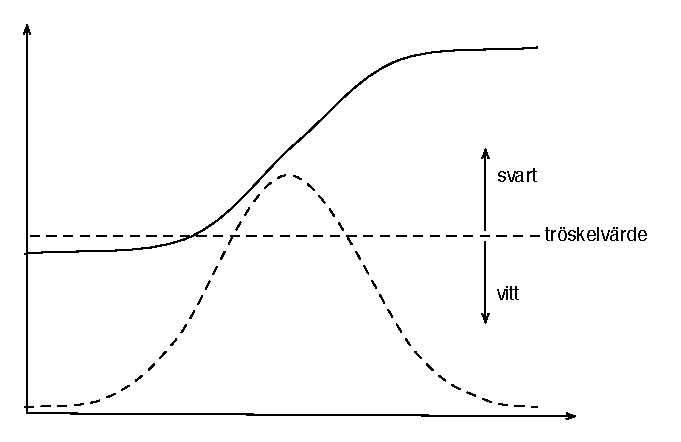
\includegraphics[width=0.9\textwidth]{../img/w13-assignment-imageprocessing/derivatabild2.pdf}
\caption { En funktion (heldragen linje) och dess derivata (streckad linje).}
\label{fig:imageprocessing:sobelfilter:derivatabild}
\end{figure}

I figur~\ref{fig:imageprocessing:sobelfilter:derivatabild} visas en funktion $f$ (heldragen linje) och funktionens derivata $f'$ (streckad linje). Vi ser att där funktionen gör ett ''hopp'' så får derivatan ett stort värde. Om funktionen representerar intensiteten hos pixlarna längs en linje i x-led eller y-led så motsvarar ''hoppen'' en kontur i bilden. Om man sedan bestämmer sig för att pixlar där derivatans värde överstiger ett visst tröskelvärde ska vara svarta och andra pixlar vita så får man en bild med bara konturer. 

Nu är ju intensiteten hos pixlarna inte en kontinuerlig funktion som man kan derivera enligt vanliga matematiska regler. Men man kan approximera derivatan, till exempel med följande formel:

\begin{displaymath}
f'(x) \approx \frac{f(x+h) - f(x-h)}{2h}
\end{displaymath}

(Om man här låter $h$ gå mot noll så får man definitionen av derivatan.) Uttryckt i Scala och matrisen \code{intensity} så får man:

\begin{Code}
val derivative = (intensity(i)(j+1) - intensity(i)(j-1)) / 2
\end{Code}

Allt detta kan man uttrycka med hjälp av faltning. 

\begin{enumerate} 
	\item Beräkna intensitetsmatrisen med metoden \code{computeIntensity}.
	\item Falta varje punkt i intensitetsmatrisen med två kärnor:
$$
X\_SOBEL =
\begin{pmatrix}
  -1 & 0 & 1 \\
  -2 & 0 & 2 \\
  -1 & 0 & 1 \\
\end{pmatrix}
Y\_SOBEL =
\begin{pmatrix}
  -1 & -2 & -1 \\
  0 & 0 & 0 \\
  1 & 2 & 1 \\
\end{pmatrix}
$$
	Använd metoden \code{convolve} med vikten 1. Koefficienterna i matrisen $X\_SOBEL$ uttrycker derivering i x-led, i $Y\_SOBEL$ faltning i y-led. För att förklara varför koefficienterna ibland är 1 och ibland 2 måste man studera den bakomliggande teorin noggrant, men det gör vi inte här.
	\item Om resultaten av faltningen i en punkt betecknas med \code{sx} och \code{sy} så får man en indikator på närvaron av en kontur med \code{math.abs(sx) + math.abs(sy)}. Absolutbelopp behöver man eftersom man har negativa koefficienter i faltningsmatriserna. 
	\item  Sätt pixeln till svart om indikatorn är större än tröskelvärdet, till vit annars. Tröskelvärdet bestäms av \code{paramValue}. 
\end{enumerate}

Skriv en klass \code{SobelFilter} som implementerar denna algoritm.

\begin{figure}[H]
\begin{center}
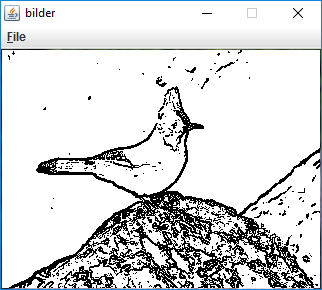
\includegraphics[width=0.6\textwidth]{../img/w13-assignment-imageprocessing/sobeljay.png}
\caption { Exempel på en bild där ett Sobelfilter applicerats med ett parametervärde på 150.}
\label{fig:imageprocessing:sobelfilter:sobel}
\end{center}
\end{figure}


\Task Implementera \code{FilterList} enligt specifikationerna ovan.

\Task Implementera \code{FilterChooser} enligt specifikationerna ovan.

\Task Knyt ihop allt i \code{ImageProcessing}-objektet som du skapade innan. Utskrifterna ska se ut på följande sätt:

{\setlength{\parindent}{0cm}

 Välj en av följande bilder genom att mata in en siffra\newline

0. boy.jpg\newline
1. car.jpg\newline
2. duck.jpg\newline
3. facade.jpg\newline
4. jay.jpg\newline
5. moon.jpg\newline
6. obidos.jpg\newline
7. sgrada.jpg\newline
8. shuttle.jpg\newline
Ditt val: \textbf{1}\newline
Bild car.jpg laddad\newline
0. för Vanligt-filter\newline
1. för Blått-filter\newline
2. för Krypterat-filter\newline
3. för Inverterat-filter\newline
4. för Grått-filter\newline
5. för Kontrast-filter\newline
6. för Gauss-filter\newline
7. för Sobel-filter\newline
8. om du inte vill använda fler filter\newline
Välj ett filter \textbf{1}\newline
Välj ett filter \textbf{8}\newline
Välja ny bild? (y/n) \textbf{n}\newline
}

Tänk på att användaren kan mata in otillåtna värden. Detta ska hanteras på lämpligt sätt.

\subsection{Frivilliga extrauppgifter}

\Task \textbf{Kontrastfilter.} Om man applicerar kontrastfiltrering på en färgbild så kommer bilden att konverteras till en gråskalebild. (Man kan naturligtvis förbättra kontrasten i en färgbild och få en färgbild som resultat. Då behandlar man de tre färgkanalerna var för sig.) Många bilder lider av alltför låg kontrast. Det beror på att bilden inte utnyttjar hela det tillgängliga området 0–255 för intensiteten. Man får en bild med bättre kontrast om man ''töjer ut'' intervallet enligt följande formel (lineär interpolation):

\begin{Code}
val newIntensity = 255 * (intensity - 45) / (225 - 45)
\end{Code}

Som synes kommer en punkt med intensiteten 45 att få den nya intensiteten 0 och en punkt med intensiteten 225 att få den nya intensiteten 255. Mellanliggande punkter sprids ut jämnt över intervallet \code{[0, 255]}. För punkter med en intensitet mindre än 45 sätter man den nya intensiteten till 0, för punkter med en intensitet större än 225 sätter man den nya intensiteten till 255. Vi kallar intervallet där de flesta pixlarna finns för \code{[lowCut, highCut]}. De punkter som har intensitet mindre än \code{lowCut} sätter man till 0, de som har intensitet större än \code{highCut} sätter man till 255. För de övriga punkterna interpolerar man med formeln ovan (45 ersätts med \code{lowCut}, 225 med \code{highCut}).

Det återstår nu att hitta lämpliga värden på \code{lowCut} och \code{highCut}. Detta är inte något som kan göras helt automatiskt, eftersom värdena beror på intensitetsfördelningen hos bildpunkterna. Man börjar med att beräkna bildens intensitetshistogram, dvs hur många punkter i bilden som har intensiteten 0, hur många som har intensiteten 1, . . . , till och med 255.

I de flesta bildbehandlingsprogram kan man sedan titta på histogrammet och interaktivt bestämma värdena på \code{lowCut} och \code{highCut}. Så ska vi dock inte göra här. I stället bestämmer vi oss för ett procenttal \code{cutOff} (som bestäms av \code{paramValue}) och beräknar \code{lowCut} så att \code{cutOff} procent av punkterna i bilden har en intensitet som är mindre än \code{lowCut} och \code{highCut} så att \code{cutOff} procent av punkterna har en intensitet som är större än \code{highCut}.

Exempel: antag att en bild innehåller 100 000 pixlar och att \code{cutOff} är 1.5. Beräkna bildens intensitetshistogram i en array
\begin{Code} 
val histogram = Array[Int](256)
\end{Code}

Beräkna \code{lowCut} så att \code{histogram(0)} + ... + \code{histogram(lowCut)} = 0.015 * 100000 (så nära det går att komma, det blir troligen inte exakt likhet). Beräkna \code{highCut} på liknande sätt.

Sammanfattning av algoritmen:
\begin{enumerate}
	\item Beräkna intensiteten hos alla punkterna i bilden, lagra dem i en \code{short}-matris. Använd den färdigskrivna metoden \code{computeIntensity}.
	\item Beräkna bildens intensitetshistogram.
	\item Parametervärdet \code{paramValue} är det värde som ska användas som \code{cutOff}.
	\item Beräkna \code{lowCut} och \code{highCut} enligt ovan.
	\item Beräkna den nya intensiteten för varje pixel enligt interpolationsformeln och lagra de nya pixlarna i \code{outPixels}.
\end{enumerate}
Skriv en klass \code{ContrastFilter} som implementerar algoritmen. I katalogen \emph{images} kan bilden \emph{moon.jpg} vara lämpliga att testa, eftersom den har låg kontrast. Anmärkning: om \code{cutOff} sätts = 0 så får man samma resultat av denna filtrering som man får av \code{GrayScaleFilter}. Detta kan man se genom att studera interpolationsformeln.

\Task \textbf{Eget filter.} Skapa ett eget filter som utnyttjar att \code{apply}-metoden tar emot en array av värden. Till exempel så kan du skicka in en array med fem värden där de två första värdena representerar ett intesitetsintervall och de tre sista värdena representerar röd-, grön- och blåkomponenterna till en färg som ska stoppas in där intensiteten hamnar utanför det givna intervallet. Ett annat alternativ kan vara att använda dig av metoder i \code{SimpleWindow} för att välja specifika pixlar på orginalbilden som sedan kan användas för att manipulera bilden i filtrets \code{apply}-metod. Valet är ditt!

%!TEX encoding = UTF-8 Unicode

%!TEX root = ../compendium.tex

%!TEX encoding = UTF-8 Unicode
\chapter{Tentaträning}\label{chapter:W14}
Koncept du ska lära dig denna vecka:
\begin{multicols}{2}\begin{itemize}[nosep,label={$\square$},leftmargin=*]
\item\end{itemize}\end{multicols}

     


\part{Appendix}         
\appendix
%!TEX encoding = UTF-8 Unicode
%!TEX root = ../compendium.tex

\chapter{Terminalfönster}\label{appendix:terminal}

\section{Vad är ett terminalfönster?}

I ett terminalfönster kan man skriva kommandon som kör program och hanterar filer. När man programmerar använder man ofta terminalkommando för att kompilera och exekvera sina program.  
 
\subsubsection{Terminal i Linux}

    \begin{figure}[!b]
    \centering
    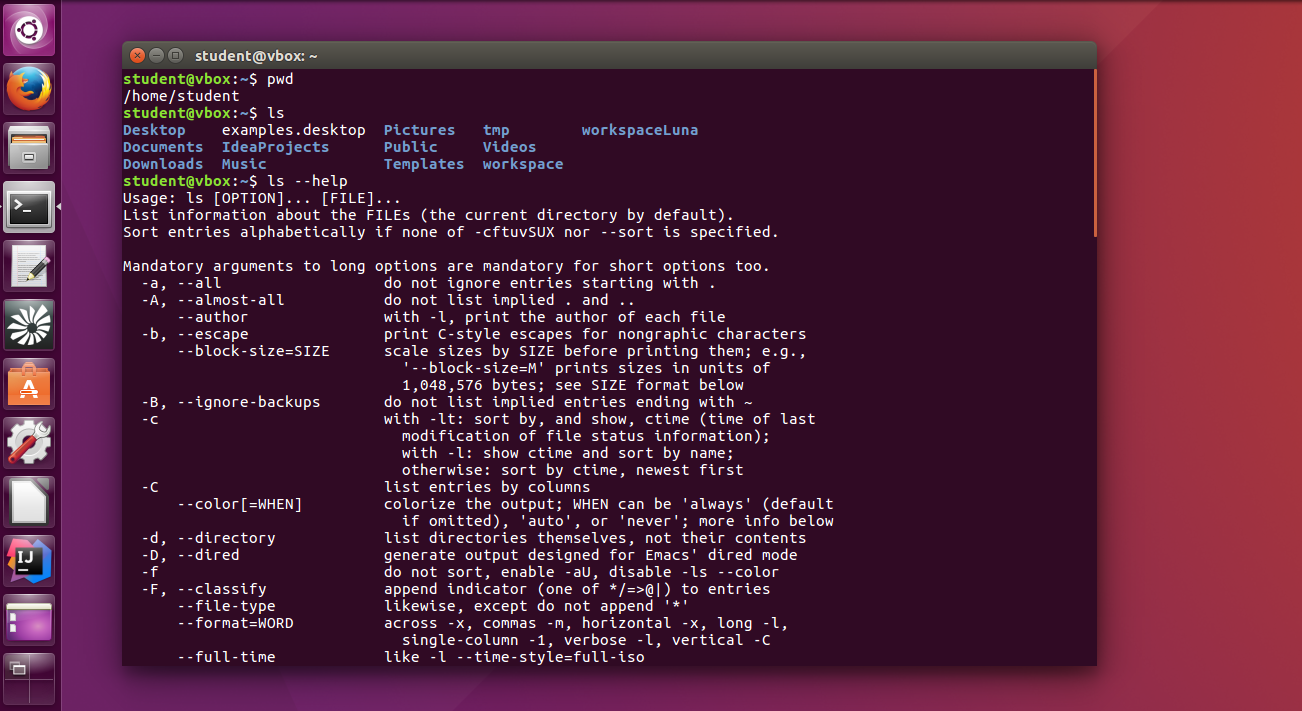
\includegraphics[width=1.0\textwidth]{../img/linux-terminal.png}
    \caption{Terminalfönster i Ubuntu öppnas med Ctrl+Alt+T.}
    \label{fig:terminal:linux}
    \end{figure}

I Ubuntu trycker du lättast \textbf{Ctrl+Alt+T} eller sök efter ''terminal'' i app-menyn.  Då öppnas ett fönster med en blinkande markör som visar att det är redo att ta emot dina textkommando. Ett exempel på kommando är \texttt{ls} som skriver ut en lista med filer i det aktuella biblioteket, så som visas i fig. \ref{fig:terminal:linux}.

Det som visas i ett terminalfönster sköts av ett \textbf{kommandoskal} \Eng{command shell}, som är redo att ta emot kommando efter en prompt som slutar med ett \texttt{\$}-tecken. När du skriver ett kommando och trycker Enter anropar kommandoskalet en kommandotolk som tolkar och utför dina kommandon. Om ett kommando inte kan tolkas, skrivs ett felmeddelande. 

Det finns många användbara kortkommando, varav de viktigaste visas i tabell \ref{fig:terminal:shortcuts}. Det är bra om du lär dig dessa kortkommandon utantill så att ditt arbete i terminalen går snabbt och smidigt.

\begin{table}[H]
\renewcommand{\arraystretch}{1.15}
\begin{tabular}{@{}r | l}
pil upp/ner & bläddra i kommandohistoriken \\
Tab & ''auto-complete'', fyll i resten baserat på vad du skrivit hittills \\
Tab Tab & två tryck på Tab listar flera alternativ, om så finnes \\
Ctrl+A & ''ahead'', flytta markören till början av raden \\
Ctrl+E & ''end'', flytta markören till slutet av raden \\
Ctrl+K & ''kill'', ta bort tecken från markören till radens slut\\
Ctrl+U & ''undo'', ta bort tecken från markören till början av raden \\
Ctrl+Y & ''yank'', sätt in det som senast togs bort\\
Ctrl+Z & ''zleep'', stoppa pågående process, skriv sedan \texttt{bg} för bakgrundskörning\\
Ctrl+L & rensa terminalfönstret\\
Ctrl+D & avsluta kommandoskalet \\
\end{tabular}
    \caption{Viktiga kortkommandon i Linux terminalfönster.}
    \label{fig:terminal:shortcuts}
\end{table}

\noindent Ctrl+C orsakar normalt ett avbrott av pågående process, men om du vill att Ctrl+C ska vara ''Copy'' som vanligt för att kopiera markerad text, kan du ställa om detta med terminalförnstrets  meny ''Edit $\rightarrow$ Keyboard Shortcuts'', eller liknande.




 
\subsubsection{PowerShell och Cmd i Microsoft Windows}
Microsoft Windows är inte Linux-baserat, men i kommandotolken \textbf{Powershell} finns alias definierade för några vanliga Linux-kommandon, inkluderat \texttt{ls}, \texttt{cd} och \texttt{pwd}. 
Du startar Powershell t.ex. genom att trycka på Windows-knappen och skriva \texttt{powershell}. 
Du kan också, medan du bläddrar bland filer, klicka på filnamnsraden överst i filbläddraren och skriva \texttt{powershell} och tryck Enter; då startas Powershell i aktuellt bibliotek. Ändra gärna typsnitt och bakgrundsfärg med hjälp av fönstrets menyer, så att det blir lättare för dig att läsa vad som skrivs.

Det finns även i Windows den ursprungliga kommandotolken \textbf{Cmd} med helt andra kommandon. Till exempel skriver man i Cmd kommandot \texttt{dir} i stället för \texttt{ls} för att lista filer. 

I Windows 10 du även köra Ubuntu-kommandoskalet, se\\ \href{http://www.omgubuntu.co.uk/2016/08/enable-bash-windows-10-anniversary-update}{http://www.omgubuntu.co.uk/2016/08/enable-bash-windows-10-anniversary-update}



\subsubsection{Terminal i Apple OS X / macOS}


Apple OS X och macOS är Unix-baserade operativsystem. De flesta vanliga terminalkommandon som fungerar i Linux fungerar också under Apple OS X och macOS. Du startar ett terminalfönster i Apples operativsystem genom att klicka på förstoringsglaset uppe till höger, skriva \texttt{terminal}, och trycka Enter.

\section{Vad är en path/sökväg?}\label{terminal:path}

När du skriver ett kommando i terminalen, eller kör vilket program som helst på din dator, behöver operativsystemet identifera i vilken fil programmets maskinkod ligger innan programmet kan köras. 

Lokaliseringe av filer sker med hjälp av en \textbf{sökväg} \Eng{path}, som anger en position i filsystemet. Ofta betraktas filsystemet som ett upp-och-ned-vänt träd, och kallas därför även ''filträdet''. Den ''översta'' positionen kallas ''rot'' \Eng{root} och betecknas med ett enkelt snedstreck \texttt{/}. Kataloger som ligger i kataloger utgör förgreningar i trädet. En sökväg pekar ut vägar genom trädet som behövs för att nå ''löven'', som utgörs av själva filerna.

Du kan se var ett program ligger i Linux med hjälp av kommandot \texttt{which} enligt nedan.\footnote{Skriv \texttt{ gcm ls } i Windows Powershell för motsvarighet till \texttt{ which ls } \\ Eller skriv \texttt{ New-Alias which get-command } för tillgång till kommandot \texttt{which} i Powershell. \\ \href{http://stackoverflow.com/questions/63805/equivalent-of-nix-which-command-in-powershell}{stackoverflow.com/questions/63805/equivalent-of-nix-which-command-in-powershell}} Listan med bibliotek i sökvägen avskiljs med snedstreck.
\begin{REPLnonum}
$ which java
/usr/lib/jvm/oracle_jdk8/bin/java
$ which ls
/bin/ls
\end{REPLnonum}

En sökväg kan vara \textbf{absolut} eller \textbf{relativ}. En absolut sökväg utgår från roten och visar hela vägen från rot till destination, t.ex. \texttt{/usr/bin/firefox}, medan en relativ sökväg utgår från aktuellt bibliotek (där du ''står'') och börjar \textit{inte} med ett snedstreck.

Alla operativsystem håller reda på en mängd olika sökvägar för att kunna hitta speciella filer i filträdet. Dessa sökvägar lagras i s.k. \textbf{miljövariabler} \Eng{environment variables}. Det finns en \textit{speciell} miljövariabel som heter kort och gott \textbf{PATH}, i vilken alla sökvägar till de program finns, som ska vara tillgängliga för din användaridentitet direkt för exekvering genom sina filnamn, \textit{utan} att man behöver ange absoluta sökvägar. 

Du kan i Linux se vad som ligger i din PATH med kommandot \code{ echo $PATH } medan man i Windows Powershell skriver \code{$env.Path} där det bara är första bokstaven som ska vara en versal. I Lunix separeras biblioteken i sökvägen med kolon, medan Windows använder semikolon.

Ibland kan du behöva uppdatera din PATH för att program som du installerat och ska bli allmänt tillgängliga. Detta görs på lite olika sätt i olika operativsystem, för Linux se t.ex. här:
\href{http://stackoverflow.com/questions/14637979/how-to-permanently-set-path-on-linux}{stackoverflow.com/questions/14637979/how-to-permanently-set-path-on-linux}

När man anger sökvägar finns några tecken med speciell betydelse:

\begin{tabular}{r  p{0.8\textwidth}}
\code|~| & ''tilde'', din hemkatalog \\
\code|/| & ''slash'', snedstreck anger filträdets rot om det finns i början av sökvägen, men utgör biblioteksavskiljare inuti sökvägen \\
\code|.| & en punkt anger aktuellt bibliotek, där du ''står'' \\
\code|..| & två punkter anger ett steg ''upp'' i filträdet \\
\code|"| & omgärda en sökväg med citationstecken, först och sist, om den innehåller annat än engelska bokstäver, t.ex. blanktecken\\
\code|\ | & \textit{backslash+blanktecken} används för att beteckna mellanslag i sökvägar som \textit{inte} omgärdas av citationstecken\\
\end{tabular}

\section{Några viktiga terminalkommando}

I tabell \ref{fig:terminal:commands} finns en lista med några viktiga terminalkommando som är bra att lära sig utantill.

En introduktion till LTH:s datorer med exempel på hur du använder vanliga Linux-kommandon finns i denna skrift \url{http://www.ddg.lth.se/perf/unix/} som används i introduktionsveckan för nybörjare på datateknikprogrammet vid LTH.

På sajten \url{http://ss64.com/} finns en mer omfattande lista med användbara terminalkommando och tillhörande förklaringarför för Linux (Bash), Windows (Powershell, Cmd) och Apple OS X.  

\begin{table}[H]
\renewcommand{\arraystretch}{1.25}
   
\begin{tabular}{@{}r | l}
\texttt{ls} & lista filer i aktuellt bibliotek (alltså där du ''står'')\\
\texttt{ls} \textit{p}  & lista filer i biblioteket  \textit{p} \\
\texttt{ls -A} & lista alla filer i aktuellt bibliotek, även gömda \\
\texttt{man ls} & manual för kommandot \texttt{ls}; testa även \texttt{man} för andra kommandon! \\
\texttt{cd} \textit{p} & ''change directory'', ändra aktuellt bibliotek till \textit{p}\\
\texttt{pwd} & ''print working directory'', skriv ut sökväg för aktuellt bibliotek \\
\texttt{cp} \textit{p1 p2} & ''copy'', kopiera filen med path \textit{p1} till en ny fil kallad \textit{p2} \\
\texttt{mv} \textit{p1 p2} & ''move'', byt namn på filen \textit{p1} till \textit{p2}  \\
\texttt{rm} \textit{p} & ''remove'', ta bort filen \textit{p}\\
\texttt{rm -r} \textit{p} & ''remove recursive'', ta bort biblioteket \textit{p} med allt innehåll; var försiktig!\\
\texttt{mkdir} \textit{p} & ''make dir'', skapa ett nytt bibliotek \textit{p}\\
\texttt{cat} \textit{p1 p2}& ''concatenate'', skriv ut hela innehållet i en eller flera filer \textit{p1 p2 etc.}\\
\texttt{less} \textit{p}& skriv ut innehållet i filen \textit{p}, en skärm i taget\\
\texttt{wget} \textit{url}&ladda ner \textit{url}, t.ex. \texttt{ wget http://cs.lth.se/pgk/ws -o ws.zip}\\
\texttt{unzip} \textit{p}& packa upp \textit{p}, t.ex. \texttt{ unzip ws.zip}\\
\end{tabular}

    \caption{Några viktiga terminalkommando i Linux. Med \textit{p}, \textit{p1}, \textit{p2}, etc.  avses en absolut eller relativ sökväg \Eng{path}, se avsnitt \ref{terminal:path}.}
    \label{fig:terminal:commands}

\end{table}


%!TEX encoding = UTF-8 Unicode
%!TEX root = ../compendium.tex

\chapter{Editera}\label{appendix:edit}
\section{Vad är en editor?}

En editor används för att redigera programkod. Det finns många olika editorer att välja på. Erfarna utvecklare lägger ofta mycket energi på att lära sig att använda favoriteditorns kortkommandon och specialfunktioner, eftersom detta påverkar stort hur snabbt kodredigeringen kan göras. 

En bra editor har \textbf{syntaxfärgning} för språket du använder, så att olika delar av koden visas i olika färger. Då går det mycket lättare att läsa och hitta i koden. 

Nedan listas några viktiga funktioner som man använder många gånger dagligen när man kodar:

\begin{itemize}
\item \textbf{Navigera}. Det finns flera olika sätt att flytta markören och bläddra genom koden. Alla editorer erbjuder sökmöjligheter, och de flesta editorer har även mer avancerade sökfunktioner där kodmönster kan identifieras och multipla sökträffar markeras över flera kodfiler. 

\item \textbf{Markera}. Att markera kod kan göras på många sätt: med piltangenter+Shift, med olika speciella menyalternativ, med mus + dubbelklick eller trippelklick, etc. I vissa editorer finns även möjlighet att ha multipla markörer så att flera rader kan editeras samtidigt.

\item \textbf{Kopiera}. Genom Copy-Paste slipper du du skriva samma sak många gånger. Kortkommandona Ctrl+C för Copy och Ctrl+V för Paste sitter i fingrarna efter ett tag. Man ska dock vara medveten om att det lätt blir fel när man kopierar en stor del som sedan ska ändras lite; många Copy-Paste-buggar kommer av att man inte är tillräckligt noggrann och ofta är det bättre att skriva från grunden i stället för att kopiera så att du hinner tänka efter medan du skriver.

\item \textbf{Klipp ut}. Genom Ctrl+X för Cut och Ctrl+V för Paste, kan du lätt flytta kod. Att skriva kod är en stegvis process där man gör många förändringar under resans gång för att förbättra och vidareutveckla koden. Att flytta på kod för att skapa en bättre struktur är mycket vanligt.

\item \textbf{Formatering}. Med indragningar, radbrytningar och nästlade block i flera nivåer får koden struktur. Många editorer kan hjälpa till med detta och har speciella kortkommandon för att ändra indragningsnivå inåt eller utåt. 

\item \textbf{Parentesmatchning}. Olika former av parenteser, \code+ ( { [ ) } ] +,  behöver matchas för att koden ska fungera; annars går kompilatorn ofta helt vilse och konstiga felmeddelanden kan peka på helt fel plats i koden. En bra kodeditor kan hjälpa dig att markera vilka parentespar som hör ihop så att du undviker att spendera för mycket tid med att leta efter en parentes som saknas eller är står i vägen.
    
\end{itemize}

I en integrerad utvecklingsmiljö, en s.k. IDE, (se appendix \ref{appendix:ide}) finns en inbyggd editor som, tack vare ett mer intimt samarbete med kompilatorn, kan erbjuda ännu fler avancerade funktioner som hjälper dig i kodarbetet. Men även när du lärt dig använda en IDE kommer du fortfarande ha stor nytta av en ''vanlig'' editor. Ofta har man flera terminalfönster igång, tillsammans med flera editorfönster och en IDE. 

\section{Välj editor}

I tabell \ref{edit:popular-editors} visas en lista med några populära editorer. Det är en stor fördel om din favoriteditor finns på flera plattformar så att du har nytta av dina förvärvade färdigheter när du behöver växla mellan olika operativsystem. 

Om du inte vet vilken du ska välja, börja med \textit{gedit}, som inte är så avancerad, men därför lätt att komma igång med. När du sedan är redo att investera din lärotid i en mer avancerad editor rekommenderas \textit{Atom}, eftersom den är öppen, gratis och finns för Linux, Windows och macOS. 

Det är är också bra att lära sig åtminstone de mest basala kommandona i editorn \textit{vim} eftersom denna  editor kan köras direkt i terminalen, även vid fjärrinloggning, och finns förinstallerad i de flesta Linux-system.


\begin{table}[t]

\renewcommand{\arraystretch}{1.25}

\begin{tabular}{@{}r | p{0.75\textwidth}}
\textit{Editor} & \textit{Beskrivning} \\ \hline

Gedit & öppen, fri och gratis; lätt att lära men inte så avancerad; finns för Linux, Windows \& macOS; är förinstallerad på LTH:s Linux-datorer och startas med kommandot \verb+gedit+ i ett terminalfönster\newline  
 \url{https://wiki.gnome.org/Apps/Gedit} \\

Atom & öppen, fri och gratis; finns för Linux, Windows, \& macOS; är förinstallerad på LTH:s Linux-datorer och startas med kommandot \verb+atom+ i ett terminalfönster; öppenkällkodsprojektet startades nyligen av GitHub och därför är Atom-editorn ännu inte lika mogen som övriga i denna lista\newline \url{https://atom.io/} \newline 
Installera Ensime som ger kraftfullt Scala-stöd i Atom: \newline \url{http://ensime.github.io/editors/atom}\\


Vim & öppen, fri och gratis; lång historik, hög inlärningströskel; finns för Linux, Windows, \& Mac; är förinstallerad på LTH:s Linux-datorer och startas med kommandot \verb+vim+ i ett terminalfönster\newline \url{http://www.vim.org/} \\

Emacs & öppen, fri och gratis; lång historik, hög inlärningströskel; finns för Linux, Windows, \& Mac; är förinstallerad på LTH:s Linux-datorer och startas med kommandot \verb+emacs+ i ett terminalfönster\newline \url{http://www.gnu.org/software/emacs/} \\

Sublime Text& sluten källkod; gratis att prova på, men programmet föreslår då och då att du köper en licens; finns för Windows, Mac, Linux. \newline
 \url{http://www.sublimetext.com/3} \\


Notepad++ & öppen, fri och gratis; finns endast för Windows; \newline \url{https://notepad-plus-plus.org/} \\


Textwrangler & sluten källkod, gratis; lätt att lära men inte så avancerad; finns endast för macOS  
\newline \url{http://www.barebones.com/products/textwrangler/} \\

\end{tabular}
    \caption{Några populära editorer. Om du inte vet vilken du ska välja, börja med att installera Gedit.}
    \label{edit:popular-editors}
\end{table}
%!TEX encoding = UTF-8 Unicode
%!TEX root = ../compendium.tex

\chapter{Kompilera och exekvera}\label{appendix:compile}

\section{Vad är en kompilator?}

En \textbf{kompilator} \Eng{compiler} är ett program som läser programtext och översätter den till exekverbar maskinkod, så som visas i figur \ref{fig:appendix:compiler}. Programtexten som kompileras kallas källkod och utgörs av text som följer reglerna för ett programmeringsspråk, till exempel Scala eller Java. 

\begin{figure}[H]
\centering
\begin{tikzpicture}[node distance=1.8cm, scale=1.5]
\node (input) [startstop] {\bf\sffamily Källkod};
\node(inptext) [right of=input, text width=2cm, xshift=1.5cm]{För\\människor};
\node (compile) [process, below of=input] {\bf\sffamily Kompilator};
%\node(explain) [right of=compile, text width=5cm, xshift=3.0cm]{Översätter från källkod till maskinkod};
\node (output) [startstop, below of=compile] {\bf\sffamily Maskinkod};
\node(outtext) [right of=output, text width=2cm, xshift=1.5cm]{För\\maskiner};
\draw [arrow] (input) -- (compile);
\draw [arrow] (compile) -- (output);
\end{tikzpicture}
    \caption{En kompilator översätter från källkod till maskinkod.}
    \label{fig:appendix:compiler}
\end{figure}




Vissa kompilatorer genererar kod som kan köras av en processor direkt, medan andra kompilatorer genererar ett mellanformat som tolkas under exekveringen. Det senare är fallet med Java och Scala, vilket möjliggör att programmet kan kompileras en gång för alla plattformar och sedan kan programmet köras på all de processorer till vilka det finns en s.k. virtuell maskin för Java \Eng{Java Virtual Machine, JVM}. Den kod som genereras av en kompilator för JVM kallas \textbf{bytekod}.

Om kompileringen inte lyckas skriver kompilatorn ut ett felmeddelande och ingen maskinkod genereras. Det är inte lätt att bygga en kompilator som ger bra felmeddelanden i alla lägen, men felmeddelandet ger oftast goda ledtrådar till felorsaken efter att man lärt sig tolka det programmeringsspråksspecifika vokabulär som kompilatorn använder.

Även om programmet kompilerar utan felmeddelande och genererar exekverbar maskinkod, är det vanligt att programmet ändå inte fungerar som det är tänkt. Ibland är det mycket svårt att lista ut vad problemet beror på och man kan behöver göra omfattande undersökningar av vad som händer under körningen, genom att t.ex. skriva ut olika variablers värden eller på annat sätt ändra koden och se vad som händer. Denna process kallas felsökning eller avlusning \Eng{debugging}, och är en väsentlig del av all systemutveckling. 

En uttömmande testning av ett större program, som kör programmets \textit{alla} möjliga exekveringsvägar, är i praktiken omöjlig att genomföra inom rimlig tid, då antalet kombinationsmöjligheter växer mycket snabbt med storleken på programmet. 
Därför är kompilatorn ett mycket viktigt hjälpmedel. Med hjälp av den analys och de kontroller som görs av kompilatorn kan många buggar, som annars vore mycket svåra att hitta, undvikas och åtgärdas i kompileringsfasen, redan \textit{innan} man exekverar programmet. 


\section{Java JDK}

Scala, Java och flera andra språk använder Java-plattformen som exekveringsmiljö. Om man inte bara vill köra program som andra har utvecklat, utan även utveckla egna program som fungerar i denna miljö, behöver man installera Java Develpment Kit (JDK). Detta utvecklingspaket innehåller flera delar, bland annat:

\begin{itemize}

\item Kompilatorn \texttt{javac} kompilerar Java-program till bytekod som lagras i klassfiler med filnamnsändelsen \texttt{.class}.

\item Exekveringsmiljön Java Runtime Enviroment (JRE) med kommandot \texttt{java} som drar igång den virtuella javamaskinen (Java Virtual Machine) som kan ladda och exekvera bytekod lagrade i klassfiler.

\item Programmet \texttt{jar} som packar ihop många sammanhörande klassfiler till en enda jar-fil som lätt kan distribueras via nätet och sedan köras med \texttt{java}-kommandot på alla maskiner med JRE. 

\item Programmet \texttt{javap} som läser klassfiler och skriver ut vad de innehåller i ett format som kan läsas av människor (ett sådant program kallas disassembler).

\item I JDK ingår också en mycket stor mängd färdiga programbibliotek med stöd för nätverkskommunikation, filhantering, grafik, kryptering och en massa annat som behövs när man bygger moderna system. 

\end{itemize}  

\noindent Du kan läsa mer om Java och dess historik här: \\
\href{https://en.wikipedia.org/wiki/Java_(programming_language)}{https://en.wikipedia.org/wiki/Java\_(programming\_language)}

\subsection{Kontrollera om du har JDK installerat}\label{appendix:compile:check-jdk}

Öppna ett terminalfönster (se appendix \ref{appendix:terminal}) och skriv (observera det avslutande c:et i \texttt{javac}):
\begin{REPLnonum}
javac -version
\end{REPLnonum}
Då ska ungefär följande skrivas ut (där siffran 101 kan vara något annat):
\begin{REPLnonum}
javac 1.8.0_101
\end{REPLnonum}
Om utskriften säger att javac saknas, installera JDK enl. nedan.

Du kanske redan har enbart Java Runtime Environment (JRE) installerad, men inte JDK. Då saknar du javakompilatorn javac m.m. och behöver installera JDK, se nedan. Du kan kolla om du har JRE genom att skriva \texttt{java -version} (alltså utan c efter java). Eller så har du redan JDK installerad men inte rätt bibliotek i din PATH; se vidare nedan ang. uppdatering av PATH.



\subsection{Installera JDK}\label{appendix:compile:install-jdk}

Det finns flera JDK-distributioner att välja mellan, varav Oracle JDK och Azul Zulu OpenJDK är två exempel. Oracle JDK har störst spridning och är förinstallerad på LTH:s datorer. För att installera JDK på din egen dator behöver du gå igenom flera steg, varav vissa behöver anpassas efter det operativsystem du kör, enligt nedan. 
På kurshemsidan under ''Verktyg'' finns kompletterande instruktioner:  \url{http://cs.lth.se/pgk/verktyg} 


Din användaridentitet behöver ha administratörsrättigheter för att du ska kunna genomföra installationen.



\subsubsection{Linux} 
För Ubuntu: läs igenom och följ sedan dessa instruktioner noga: \\ \href{http://www.webupd8.org/2012/09/install-oracle-java-8-in-ubuntu-via-ppa.html}{www.webupd8.org/2012/09/install-oracle-java-8-in-ubuntu-via-ppa.html}

För andra Linux-distributioner, kör detta i terminalen (funkar även i Ubuntu, men du får med detta kommando inte Oracles aningen snabbare JVM): \\ \texttt{sudo apt-get install openjdk-8-jdk}

\subsubsection{Windows/macOS}

\begin{enumerate}
\item Installera senaste JDK från Oracle. Om du inte har installerat JDK förr på din dator så be gärna någon kurskamrat med erfarenhet av detta att assistera dig medan du följer stegen nedan. 

\begin{enumerate}
\item Surfa till Oracles hemsida för Java SE här: \\ \url{http://www.oracle.com/technetwork/java/javase/downloads/}

\item Klicka på rubriken ''Java SE 8u101 / 8u102'' och på nästa sida klicka på knappen ''Accept License Agreement'' i listan under rubriken ''Java SE Development Kit 8u101''. (Siffrorna 101 eller 102 kan vara annorlunda om senare versioner tillkommit.)

\item Välj rätt version av operativsystem (Windows x64 eller Mac OS X). Det är viktigt att du väljer x64, d.v.s 64-bitarsvarianten som gäller för alla moderna datorer.

\item Klicka på länken och en stor fil kommer laddas ner till din dator.

\item Installera när filen laddats färdigt. 

\end{enumerate}

\item Uppdatera PATH, så att du får tillgång till alla kommando i terminalen:
\begin{itemize}
\item För Windows görs detta enklast genom att ladda ner och sedan köra denna fil genom att dubbelklicka på den: \\ \mbox{\href{https://github.com/lunduniversity/introprog/raw/master/tools/windows-jdk-set-path.bat}{github.com/lunduniversity/introprog/raw/master/tools/windows-jdk-set-path.bat}}
\item För macOS, läs här: \\ \href{https://docs.oracle.com/javase/8/docs/technotes/guides/install/mac_jdk.html}{docs.oracle.com/javase/8/docs/technotes/guides/install/mac\_jdk.html} 
\\ \TODO finn ut bästa rådet att sätta path på mac

\item Om något krånglar, be om hjälp. Om du behöver mer detaljer om PATH-uppdatering för java, läs här:  \href{https://java.com/sv/download/help/path.xml}{java.com/sv/download/help/path.xml} \\
Om du kör engelska menyer byt \texttt{sv} mot \texttt{en} i adressen ovan.  Du kan ta reda på vilken katalog som ska läggas in sist i din PATH genom att bläddra bland dina systemfiler och undersöka var JDK har installerats; i Windows antagligen något liknande detta (kolla exakt vilket versionsnummer du har): \code|C:\Program Files\Java\jdk1.8.0_101\bin|
\end{itemize}

\item Starta om datorn. Det är först efter att en ny användarinloggning initierats, som PATH-tilldelningen får effekt.

\item Kontrollera att \texttt{javac} fungerar enligt avsnitt \ref{appendix:compile:check-jdk}.
\end{enumerate}


\section{Scala}

Scala använder JDK som exekveringsmiljö, men erbjuder ytterligare verktyg specifika för Scala. I utvecklingspaketet för Scala ingår bl.a. kompilatorn \texttt{scalac} och även ett interaktivt kommandoskal kallat Scala REPL där du kan testa din Scala-kod rad för rad och se vad som händer direkt. 

De flesta av kursens övningar görs i Scala REPL, medan laborationerna kräver kompilering av lite större program.

Du hittar mer om Scalas historik och annan bakgrundsinformation här: \mbox{%
 \href{https://en.wikipedia.org/wiki/Scala_(programming_language)}{en.wikipedia.org/wiki/Scala\_(programming\_language)}
}

\subsection{Installera Scala}

Scala finns förinstallerat på LTH:s datorer. Du installerar Scala-kompilatorn och den interaktiva kodexperimentmiljön Scala REPL på din egen dator enligt nedan. 

\begin{enumerate}
\item Kontrollera att du har JDK installerad enligt avsnitt \ref{appendix:compile:check-jdk} och installera vid behov enligt avsnitt \ref{appendix:compile:install-jdk}.
\item Surfa till denna hemsida för nedladdning av Scala 2.11.8: \\ \url{http://scala-lang.org/download/2.11.8.html}
\item Klicka på ''Download'' av den variant som är relevant för ditt operativsystem och spara filen:

\begin{enumerate}
\item \textbf{Linux Ubuntu}: Filen heter \texttt{scala-2.11.8.deb} och installeras genom att dubbelklicka på filen eller via terminalkommandot:\\ \code{sudo apt install ~/Downloads/scala-2.11.8.deb} \\ Anpassa sökvägen ovan efter var du sparade filen. 
\item \textbf{Windows}: Filen heter \texttt{scala-2.11.8.msi} och installationen startas med ett dubbelklick. Följ instruktionerna. Installationsprogrammet uppdaterar även din PATH åt dig och kommandot \texttt{scala} bör fungera efter omstart.
\item \textbf{macOS}: Filen heter \texttt{scala-2.11.8.tgz} och kan packas upp på lämpligt ställe med terminalkommandot \texttt{tar -xvzf scala-2.11.8.tgz} och sedan är det underkatalogen \texttt{bin} som ska inkluderas i din PATH. \TODO klura ut säkraste rådet för PATH-uppdatering på mac.
\end{enumerate}
\end{enumerate}
Kontrollera, efter ev. omstart, att terminalkommandot \texttt{scala} nu kan användas för att starta Scala REPL på din dator:
\begin{REPLnonum}
$ scala
Welcome to Scala 2.11.8 (Java HotSpot(TM) 64-Bit Server VM, Java 1.8.0_101).
Type in expressions for evaluation. Or try :help.

scala> val msg = "hej"
msg: String = hej

scala> println(msg)
hej

scala> 
\end{REPLnonum}
 

\subsection{Scala Read-Evaluate-Print-Loop (REPL)}\label{appendix:compile:REPL}

För många språk, t.ex. Scala och Python, finns det ett interaktivt program ämnat för terminalen som gör det möjligt att exekvera enstaka programrader och direkt se effekten. Ett sådant program kallas \textit{Read-Evaluate-Print-Loop} (REPL), eftersom det läser  och tolkar en rad i taget. Resultatet av evalueringen av din kod skrivs ut i terminalen och därefter är kommandoskalet redo för nästa kodrad.

Kursens övningar bygger till stor del på att du använder Scala REPL för att undersöka principer och begrepp som ingår i kursen genom dina egna kodexperiment. Även när du på labbarna utvecklar större program med en editor och en IDE, är det bra att ha Scala REPL till hands. Då kan du klistra in delar av programmet du håller på att utveckla i Scala REPL och stegvis utveckla delprogram, som till slut fungerar så som du vill. 

I Scala REPL får du se typinformation för variabler och metoder, vilket är till stor hjälp när man försöker lista ut vad en kodrad innebär. Genom att öva upp din förmåga att dra nytta av Scala REPL, kommer din produktivitet öka.

Du startar Scala REPL med kommandot \texttt{scala} och skriver Scala-kod efter prompten \texttt{scala>} och kompilering+exekvering sker när du trycker Enter.
\begin{REPLnonum}
$ scala
Welcome to Scala 2.11.8 (Java HotSpot(TM) 64-Bit Server VM, Java 1.8.0_101).
Type in expressions for evaluation. Or try :help.

scala> def inc(x: Int) = x + 1
inc: (x: Int)Int

scala> inc(inc(inc(1)))
res8: Int = 4

scala> 
\end{REPLnonum}

Med kommandot \texttt{:paste} försätter du Scala REPL i inklistringsläge \Eng{paste mode} och du kan då med Ctrl+V (eller Ctrl+Shift+V, eller eventuellt högerklick med musen, beroende på hur ditt terminalprogram är inställt och vilket operativsystem du kör) klistra in större sjok av kod. När du med Ctrl+D avslutar inklistringsläget och Scala REPL tolkar alla raderna på en gång. Kommandot  \texttt{:paste} kan förkortas till  \texttt{:pa}, så som visas nedan. Koden mellan raderna som börjar med \texttt{//} klistrades in av användaren efter att ha kopierats från en editor i ett annat fönster.

\begin{REPLnonum}
scala> :pa
// Entering paste mode (ctrl-D to finish)

case class Point3D(val pos: (Int, Int, Int))
object Point3D {
  def apply(x: Int, y: Int) = new Point3D(x,y,0)
}

// Exiting paste mode, now interpreting.

defined class Point3D
defined object Point3D

scala> Point3D(1,2)
res6: Point3D = Point3D((1,2,0))

scala> 
\end{REPLnonum}

Många av de kortkommandon som fungerar i terminalens kommandoskal, fungerar också i Scala REPL. Gå gärna igenom listan i tabell \ref{fig:terminal:shortcuts} på sidan \pageref{fig:terminal:shortcuts}, och testa vad som händer i Scala REPL. Om du tränar upp din fingerfärdighet med dessa kortkommandon, går ditt arbete i Scala REPL väsentligt snabbare. 

Med kommandot \texttt{:help} får du se en lista med specialkommandon för Scala REPL, inklusive de som återfinns i tabell \ref{fig:repl:shortcuts} på sidan \pageref{fig:repl:shortcuts}.

\begin{table}
\renewcommand{\arraystretch}{1.25}\centering
\begin{tabular}{r | c | l}
\textit{Kommando} & \textit{Förk.} & \textit{Beskrivning} \\ \hline 
 \texttt{:help}     & \texttt{:he} & visa lista med kommando och förklaringar\\
 \texttt{:paste}     & \texttt{:pa} & växla till inklistringsläge \Eng{paste mode}\\
 \texttt{:paste} \textit{path}    & \texttt{:pa} \textit{path} & klistra in en hel fil, t.ex. \code|:pa util/mio.scala|\\
 \texttt{:quit} & \texttt{:q}  & avsluta Scala REPL \\ 
 \texttt{:require} \textit{path} & \texttt{:req} \textit{path} & jar-fil till classpath, t.ex. \texttt{:req lib/cslib.jar}\\
 
 \texttt{:type} & \texttt{:t}  & visa typ med -v för ''verbose'', t.ex. \code|:t -v 42.0| \\ 

 \texttt{:warnings} & \texttt{:w}  & visa beskrivning av ev. varningar \\ 

\end{tabular}
    \caption{Några vanliga kommandon i Scala REPL.}
    \label{fig:repl:shortcuts}
\end{table}






%!TEX encoding = UTF-8 Unicode
%!TEX root = ../compendium.tex

\chapter{Integrerad utvecklingsmiljö}\label{appendix:ide}

\section{Vad är en integrerad utvecklingsmiljö?}

En integrerad utvecklingsmiljö \Eng{integrated development environment, IDE} samlar ett flertal verktyg, inklusive en avancerad \textbf{editor} (se appendix \ref{appendix:edit}), för att skapa, köra och testa program. Det finns flera utvecklingsmiljöer att välja mellan, som kan användas för både Scala och Java.

En IDE ger stöd för \textbf{kodkomplettering} \Eng{code completion} där tillgängliga metoder visas i en lista och resten av ett namn kan fyllas i automatiskt efter att du skrivit de första bokstäverna i namnet. En IDE kan hjälpa dig med formattering och även skapa skelettkod utifrån \textbf{kodmallar} \Eng{code templates}. Med \textbf{felindikering} \Eng{error highlighting} får du understrykning av vissa fel direkt i koden och ibland kan du även få hjälp med förslag på åtgärder för att rätta till enkla fel. Funktioner för \textbf{avlusning} \Eng{debugging} hjälper dig att felsöka medan du kör din kod. Med funktioner för \textbf{omstrukturering} \Eng{refactoring} av kod får du hjälp av editorn i samarbete med kompilatorn att göra omfattande strukturförändringar i många kodfiler samtidigt, t.ex. namnbyten med hänsyn taget till språkets synlighetsregler.  

Alla dessa avancerade funktioner kan öka produktiviteten avsevärt, men samtidigt tar de tid att lära sig och en IDE kan kräva mycket datorkraft och viss väntetid jämfört med en vanlig, fristående editor. I början kan all funktionalitet upplevas som överväldigande och det kan vara svårt att hitta i alla menyer och inställningar. Ska man bara skriva ett litet, enkelt program, eller göra några mindre ändringar, är det många som föredrar en fristående, snabbstartad kodeditor före en fullfjädrad, tungrodd IDE. Å andra sidan kan en IDE med kodkomplettering vara till stor hjälp när man ska lära sig ett nytt api och experimentera med en okänd kodmassa.

I kursen använder vi flera utvecklingsmiljöer. På första labben använder vi Kojo (avsnitt \ref{appendix:ide:kojo}) som är en IDE speciellt anpassad på nybörjare. I laborationerna senare i kursen kan du välja att använda någon av de professionella utvecklingsmiljöerna Eclipse (avsnitt \ref{appendix:ide:eclipse}) eller IntelliJ (avsnitt \ref{appendix:ide:intellij}). Om du inte vet vilken du ska välja, börja med att prova Eclipse.


\newpage

\section{Kojo}\label{appendix:ide:kojo}

Kojo%
\footnote{\href{https://en.wikipedia.org/wiki/Kojo_(programming_language)}{en.wikipedia.org/wiki/Kojo\_(programming\_language)}}
 är en integrerad utvecklingsmiljö för Scala som är speciellt anpassad för nybörjare i programmering. Kojo används i LTH:s Science Center Vattenhallen för utbildning av grundskolelärare i programmering och vid skolbesök och annan besöksverksamhet, i vilken lärare och studenter vid LTH arbetar som handledare. Kojo är fri öppenkällkod och utvecklingen leds av Lalit Pant.

Kursens första laboration genomförs med hjälp av Kojo, men Kojo kan med fördel användas som komplement till Scala REPL och annan IDE under hela kursens gång. Medan Scala REPL lämpar sig för korta kodsnuttar, och en fullfjädrad, professionell IDE har funktioner för att hantera riktigt stora programmeringsprojekt, passar Kojo bra för mellanstora program. I Kojo finns även lätttillgängliga bibliotek som gör tröskeln lägre att programmera rörlig grafik och enkla spel.   


\begin{figure}[H]
\centering
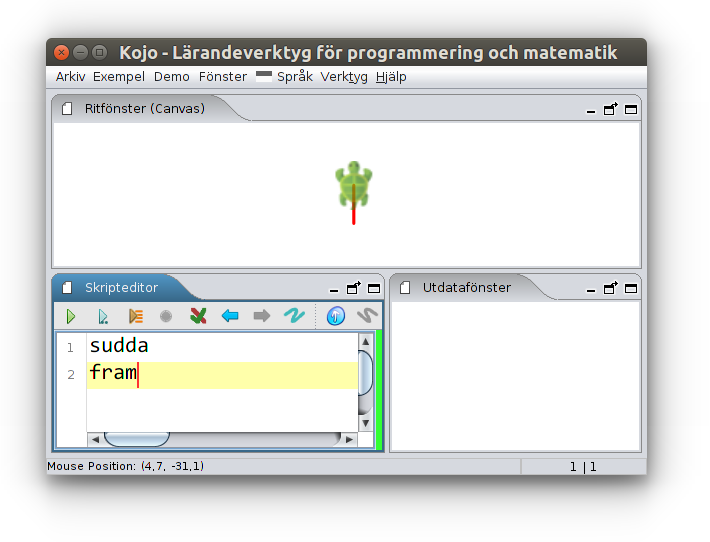
\includegraphics[width=0.8\textwidth]{../img/kojo/kojo.png}
\caption{Den nybörjarvänliga utvecklingsmiljön Kojo för Scala på svenska.}
\label{fig:appendix:ide:kojo}
\end{figure} 

\subsection{Installera Kojo}

Kojo är förinstallerat på LTH:s datorer och körs igång med kommandot \texttt{kojo}. För instruktioner om hur du installerar Kojo på din egen dator se här:\\
\href{http://www.lth.se/programmera/installera/}{lth.se/programmera/installera}

Kojo kräver att \texttt{java} finns på din dator. Eftersom du behöver tillgång till JDK i kursen, är det lika bra att installera hela JDK direkt (och inte bara JRE, så som beskrivs å länken ovan); se vidare hur du gör detta i avsnitt \ref{appendix:compile:install-jdk}. 
%\href{http://www.kogics.net/kojo-download}{www.kogics.net/kojo-download}


\subsection{Använda Kojo}

När du startar Kojo första gången, välj ''Svenska'' i språkmenyn och starta om Kojo. Därefter fungerar grafikfunktionerna på svenska enligt tabell \ref{table:kojo:functions}. När du startat om Kojo inställt på Svenska ser programmet ut ungeför som i figur \ref{fig:appendix:ide:kojo} på sidan \pageref{fig:appendix:ide:kojo}.


Det finns ett antal användbara kortkommando som du hittar i menyerna i Kojo. Undersök speciellt Ctrl+Alt+Mellanslag som ger autokomplettering baserat på det du börjat skriva.


{\small\renewcommand{\arraystretch}{1.45}
\begin{longtable}{@{}p{0.42\textwidth} p{0.55\textwidth}}

\caption{Några av sköldpaddans funktioner. Se även \href{http://lth.se/programmera}{lth.se/programmera}}\label{table:kojo:functions}\\

\emph{Svenska/Engelska} & \emph{Vad händer?}  \\ \hline
\code|sudda| \newline \code|clear| & Ritfönstret suddas \\
\code|fram| \newline \code|forward(25)| & Paddan går framåt 25 steg. \\
\code|fram(100)| \newline \code|forward(100)| & Paddan går framåt 100 steg. \\
\code|höger| \newline \code|right(90)| & Paddan vrider sig 90 grader åt höger. \\
\code|höger(45)| \newline \code|right(45)| & Paddan vrider sig 45 grader åt höger. \\
\code|vänster| \newline \code|left(90)| & Paddan vrider sig 90 grader åt vänster. \\
\code|vänster(45)| \newline \code|left(45)| & Paddan vrider sig 45 grader åt vänster. \\
\code|hoppa| \newline \code|hop| & Paddan hoppar 25 steg utan att rita. \\
\code|hoppa(100)| \newline \code|hop(100)| & Paddan hoppar 100 steg utan att rita. \\
\code|hoppaTill(100, 200)| \newline \code|jumpTo(100, 200)| & Paddan hoppar till läget (100, 200) utan att rita. \\
\code|gåTill(100, 200)| \newline \code|moveTo(100, 200)| & Paddan vrider sig och går till läget (100, 200). \\
\code|hem| \newline \code|home| & Paddan går tillbaka till utgångsläget (0, 0). \\
\code|öster| \newline \code|setHeading(0)| & Paddan vrider sig så att nosen pekar åt höger. \\
\code|väster| \newline \code|setHeading(180)| & Paddan vrider sig så att nosen pekar åt vänster. \\
\code|norr| \newline \code|setHeading(90)| & Paddan vrider sig så att nosen pekar uppåt. \\
\code|söder| \newline \code|setHeading(-90)  | & Paddan vrider sig så att nosen pekar neråt. \\
\code|mot(100,200)| \newline \code|towards(100, 200)| & Paddan vrider sig så att nosen pekar mot läget (100, 200) \\
\code|sättVinkel(90)| \newline \code|setHeading(90)| & Paddan vrider nosen till vinkeln 90 grader. \\
\code|vinkel| \newline \code|heading| & Ger vinkelvärdet dit paddans nos pekar. \\
\code|sakta(5000)| \newline \code|setAnimationDelay(5000) | & Gör så att paddan ritar jättesakta. \\
\code|suddaUtdata| \newline \code|clearOutput| & Utdatafönstret suddas. \\
\code|utdata("hej")| \newline \code|println("hej")| & Skriver texten \texttt{hej} i utdatafönstret. \\
\code|val t = indata("Skriv")| \newline \code|val t = readln("Skriv:")| & Väntar på inmatning efter ledtexten \texttt{Skriv} och sparar den inmatade texten i t.  \\
\code|textstorlek(100)| \newline \code|setPenFontSize(100)| & Paddan skriver med jättestor text nästa gång du gör skriv. \\
\code|båge(100, 90)| \newline \code|arc(100, 90)| & Paddan ritar en båge med radie 100 och vinkel 90. \\
\code|cirkel(100)| \newline \code|circle(radie)| & Paddan ritar en cirkel med radie 100. \\
\code|synlig| \newline \code|visible| & Paddan blir synlig. \\
\code|osynlig| \newline \code|invisible| & Paddan blir osynlig. \\
\code|läge.x| \newline \code|position.x| & Ger paddans x-läge \\
\code|läge.y| \newline \code|position.y| & Ger paddans y-läge \\
\code|pennaNer| \newline \code|penDown| & Sätter ner paddans penna så att den ritar när den går. \\
\code|pennaUpp| \newline \code|penUp| & Sänker paddans penna så att den INTE ritar när den går. \\
\code|pennanÄrNere| \newline \code|penIsDown| & Kollar om pennan är nere eller inte. \\
\code|färg(rosa)| \newline \code|setPenColor(pink)| & Sätter pennans färg till rosa. \\
\code|fyll(lila)| \newline \code|setFillColor(purple)| & Sätter ifyllnadsfärgen till lila. \\
\code|fyll(genomskinlig)| \newline \code|setFillColor(noColor)| & Gör så att paddan inte fyller i något när den ritar. \\
\code|bredd(20)| \newline \code|setPenThickness(20)| & Gör så att pennan får bredden 20. \\
\code|sparaStil| \newline \code|saveStyle| & Sparar pennans färg, bredd och fyllfärg. \\
\code|laddaStil| \newline \code|restoreStyle| & Laddar tidigare sparad färg, bredd och fyllfärg. \\
\code|sparaLägeRiktning| \newline \code|savePosHe| & Sparar pennans läge och riktning \\
\code|laddaLägeRiktning| \newline \code|restorePosHe| & Laddar tidigare sparad riktning och läge \\
\code|siktePå| \newline \code|beamsOn| & Sätter på siktet. \\
\code|sikteAv| \newline \code|beamsOff| & Stänger av siktet. \\
\code|bakgrund(svart)| \newline \code|setBackground(black)| & Bakgrundsfärgen blir svart. \\
\code|bakgrund2(grön,gul)| \newline \code|setBackgroundV(green, yellow)| & Bakgrund med övergång från grönt till gult. \\
\code|upprepa(4){fram; höger}| \newline \code|repeat(4){forward; right}| & Paddan går fram och svänger höger 4 gånger. \\
\code|avrunda(3.99)| & Avrundar 3.99 till 4.0 \\
\code|slumptal(100)| & Ger ett slumptal mellan 0 och 99. \\
\code|slumptalMedDecimaler(100)| & Ger ett slumptal mellan 0 och 99.99999999 \\
\code|systemtid| & Ger nuvarande systemklocka i sekunder. \\
\code|räknaTill(5000)| & Kollar hur lång tid det tar för din dator att räkna till 5000. \\



\hline
\end{longtable}
}%end small

\noindent Scala-koden för den svenska paddans api finns här: \\
\href{https://bitbucket.org/lalit_pant/kojo/src/tip/src/main/scala/net/kogics/kojo/lite/i18n/svInit.scala}{bitbucket.org/lalit\_pant/kojo/src/tip/src/main/scala/net/kogics/\\kojo/lite/i18n/svInit.scala}




\newpage

\section{Eclipse och ScalaIDE}\label{appendix:ide:eclipse}

Eclipse%
\footnote{\href{https://en.wikipedia.org/wiki/Eclipse_(software)}{en.wikipedia.org/wiki/Eclipse\_(software)}}
är en professionell IDE som stödjer många olika programmeringsspråk. Eclipse är skriven i Java och bygger vidare på ett utvecklingsprojekt som initierades av IBM. Eclipse är ett fritt och öppet projekt som numera kontrolleras av en oberoende stiftelse.

Till Eclipse finns en insticksmodul \Eng{plug-in} som kallas ScalaIDE och erbjuder stöd för Scala med tillhörande standardbibliotek.

Eclipse är en omfattande och avancerad programmeringsmiljö med många funktioner och inställningar. Det finns även en omfattande uppsättning insticksmoduler och tilläggsprogram som underlättar utveckling av t.ex. webbprogram, databaser och mycket annat. 

I detta avsnitt ges länkar till installation samt tips om hur du kommer igång med att använda Eclipse och ScalaIDE. Det går ganska snabbt att lära sig grunderna, men det kräven en viss ansträngning att lära sig de mer avancerade funktionerna. Det finns omfattande resurser på nätet som hjälper dig vidare. 


\subsection{Installera Eclipse Mars och ScalaIDE}\label{appendix:ide:eclipse:install}

Eclipse med ScalaIDE är förinstallerat på LTH:s datorer och startas med kommandot \texttt{scalaide} i ett terminalfönster.

ScalaIDE fungerar med Eclipse-versionerna \textit{Luna} och \textit{Mars} (men i skrivande stund fungerar ScalaIDE ännu \textit{inte} med den allra senaste versionen kallad \textit{Neon}). 

För att installera ScalaIDE på din egen dator, följ nedan instruktioner: 

\begin{enumerate}
\item Kontrollera enligt avsnitt \ref{appendix:compile:check-jdk} att du har \texttt{java} installerat och installera vid behov JDK enligt avsnitt \ref{appendix:compile:install-jdk}.

\item Installera Eclipse version \textbf{Mars}, varianten för \textbf{Java Developers} som återfinns på denna sida: \\ \url{https://www.eclipse.org/downloads/packages/release/Mars/2} \\ som är den \textit{andra} varianten i listan (alltså inte Java EE). Följ dessa steg:
\begin{enumerate}
\item Klicka på den \textbf{64-bit}-variant som passar ditt operativsystem.
\item Filen som laddas ner heter något som liknar (beroende på OS): \\ \texttt{eclipse-java-mars-2-win32-x86\_64.zip} 
\\ Det kan ta lång tid att ladda ner filen som är på ca 170MB. Om du klickar på \textit{''select a mirror''} kan du välja en svensk sajt för att ladda ner snabbare. 

\item Dubbelklicka på filen för att packa upp den, vilket kan ta många minuter. Du får, när upppackningen är klar, ett bibliotek med en fungerande Eclipse-installation som du kan placera var du vill. Kör du Windows, lägg den förslagsvis här:\\ 
\code|C:\eclipse\eclipse-java-mars-2-win32-x86_64|

\item för Ubuntu Linux finns kompletterande installationsanvisningar här, som ger dig en ikon i app-menyn m.m.: 
\\ \url{http://askubuntu.com/questions/26632/how-to-install-eclipse}
\end{enumerate}

\item Installera Scala IDE inifrån%
\footnote{Det finns på ScalaIDE-hemsidan möjlighet att ladda ner en Eclipse-variant med färdiginstallerad ScalaIDE-plugin, men då får du i skrivande stund den gamla versionen Eclipse \textit{Luna}, varför du rekommenderas att, enligt instruktionerna här, själv installera ScalaIDE inifrån Eclipse \textit{Mars}, som är den senaste Eclipse-versionen för vilken ScalaIDE fungerar.}
 Eclipse enligt nedan steg:
\begin{enumerate}
\item Starta Eclipse, t.ex. genom att köra igång den exekverbara filen som ligger i underbiblioteket \texttt{eclipse}, i Windows heter den \texttt{eclipse.exe} medan den exekverbara filen i Linux heter \texttt{eclipse} utan filändelse.

\item Välj i frågerutan som dyker upp, någon plats för \textit{workspace} (kvittar vilken just nu, kan ändras senare).

\item Klicka på menyn \textit{Help} $\rightarrow$ \textit{Install new software}.

\item Klicka på \textit{Add}-knappen till höger och skriv: \\ \textit{''ScalaIDE for Scala 2.11''} i \textit{Name}-fältet och ange denna adress i \textit{Location}-fältet: \\
  {\small\mbox{\url{http://download.scala-ide.org/sdk/lithium/e44/scala211/stable/site}}} \\
  och klicka \textit{OK}.
  
\item Du får nu upp en lista med alternativ. Kryssa för alternativet
\\ {\frame{\checkmark}}~~\textit{Scala IDE for Eclipse} \\ och klicka \textit{Next} och sedan \textit{Next} igen och acceptera licensvillkoren och klicka \textit{Finish}.

\item Låt installationen ta sin tid och starta sedan om Eclipse när installationen är färdig. 

\item När Eclipse är igång igen visas en dialog som föreslår att du ska köra \textit{Setup Diagnostics}. Gör detta och välj \textit{Use recommended default settings}. Ändra även i filen \textbf{eclipse.ini} för höja den övre minnesgränsen. Det gör du genom att ändra på den rad i filen som börjar med \texttt{-Xmx}. Hur mycket du ska tillåta som max beror på hur mycket minne du har, men ge minst 1 gigabyte för smidig körning, genom att skriva så här på relevant rad i filen \textbf{eclipse.ini}: \\
\texttt{-Xmx1G } \\


\item Kompletterande information finns här, inklusive en video som visar installationsproceduren och hur man kommer igång med ett ''hello world''-program: \\ \url{http://scala-ide.org/download/current.html}


\end{enumerate}


\end{enumerate}

\noindent I nästa avsnitt beskrivs några rekommenderade anpassningar som du kan göra bland de omfattande inställningsmöjligheterna för Eclipse.

\newpage

\subsection{Anpassa Eclipse och ScalaIDE}\label{subsection:appendix:ide:eclipse:tweaks}

\newcommand\Menu[1]{\textit{#1}}
\newcommand\MenuArrow[1]{\Menu{#1}~$\rightarrow$~}
\newcommand\FramedCheckmark[1]{~\frame{\checkmark}~~\textbf{#1}}
\newcommand\FramedUnchecked[1]{$\Box$~\textbf{#1}}
\newcommand\Button[1]{\fbox{\textbf{#1}}}
\newcommand\EclipsePrefs{\MenuArrow{Window}\MenuArrow{Preferences}}
\newcommand\EclipsePrefsGeneral{\EclipsePrefs\MenuArrow{General}}


Förutom maxminneshöjningen i filen \texttt{eclipse.ini}, som finns i installationskatalogen för Eclipse, till minst \texttt{-Xmx1G } (se föregående avsnitt), är det bra att göra några ytterligare anpassningar av Eclipse och ScalaIDE för att få en snabbare och smidigare utvecklingsmiljö. Du hittar inställningarna i menyn \EclipsePrefs ... uppe till höger i Eclipse-fönstret.



\begin{enumerate}
\item \EclipsePrefsGeneral 
\\ Markera \FramedCheckmark{Show Heap Status} så får du se minnesanvändningen i en liten ruta i nederdelen av fönstret, vilket hjälper dig att upptäcka om minnesbegränsningen i filen \texttt{eclipse.ini} är en flaskhals vid stora projekt och många öppna fönster. Klicka sedan \Button{Apply} längst ner.

\item \label{item:scala-perspective} \EclipsePrefsGeneral\MenuArrow{Editors}\MenuArrow{Perspective}  
\\ Markera \textit{Scala} i listan med perspektiv och klicka på knappen 
 \\ \Button{Make default} till höger och sedan på knappen \Button{Apply} längst ner.

\item \EclipsePrefsGeneral\MenuArrow{Editors}\MenuArrow{TextEditors}
\\ Markera \FramedCheckmark{Insert spaces for tabs} så att du slipper specialtecken som kan tolkas olika av olika editorer. Klicka sedan \Button{Apply} längst ner.

\item \EclipsePrefsGeneral\MenuArrow{Editors}\MenuArrow{TextEditors}
\\ \MenuArrow{Spelling} Avmarkera \FramedUnchecked{Enable spell checking} för att slippa att svenska namn och svenska kommentarer markeras som felstavade. Om du senare jobbar med ett projekt helt på engelska, kan du med fördel markera denna kryssruta igen. Klicka sedan \Button{Apply} längst ner.

\item \EclipsePrefsGeneral\MenuArrow{Editors}\MenuArrow{Webbrowser}
\\ Markera \FramedCheckmark{Use external web browser} för att köra din vanliga webbläsare när du klickar på länkar. Klicka sedan \Button{Apply} längst ner.
  
\item  \EclipsePrefs\MenuArrow{Scala}\MenuArrow{Compile}
\\ I fliken \textbf{Standard} markera dessa kryssrutor för att få extra varningar: \\
\begin{tabular}{l @{}l @{}l}
\textit{deprecation} & \FramedCheckmark{} & varnar vid användning av föråldrad kod som snart utgår \\
\textit{feature}     & \FramedCheckmark{} & påminner om import vid användning av avancerad kod  \\
\textit{unchecked}   & \FramedCheckmark{} & ger tips vid speciella problem med generiska typer \\
\end{tabular}\\
och klicka sedan på knappen \Button{Apply} längst ner.

\item \EclipsePrefs\MenuArrow{Java}\MenuArrow{Compiler}\MenuArrow{Errors/Warnings}
\\ Veckla ut listan \textbf{Potential programming problems} och sätt \textbf{Resource leak} till alternativet \textbf{Ignore}, så slipper du varningar vid användning \jcode{Scanner} i Java. Klicka sedan \Button{Apply} längst ner.

\end{enumerate}

\noindent Ovan anpassningar är rekommenderade men inte nödvändiga och du kan gärna välja att göra andra anpassningar som passar just dig. Skriv då gärna ner vilken inställning du ändrat, så att du hittar tillbaka om du ångrar dig. 

Du hittar tips om fler inställningar för att anpassa ScalaIDE här: \\
\url{http://scala-ide.org/docs/current-user-doc/advancedsetup}



\subsection{Använda Eclipse och ScalaIDE}\label{appendix:ide:eclipse:use}

Ett grundläggande koncept i Eclipse är \textbf{workspace}. Ett workspace utgör ett arbetsområde kopplat till en katalog i ditt filsystem där du kan arbeta med ett eller flera \textbf{projekt}. Ett projekt innehåller i sin tur dina källkodsfiler och klassfiler etc. i en specifik katalogstruktur som Eclipse skapar när du editerar, kompilerar och kör dina projekt. 

\subsubsection{Starta och välja workspace}\label{subsubsection:start:eclipse}

När du startar Eclipse måste du välja vilket workspace du vill använda innan du kommer vidare. När du kör igång Eclipse första gången, klicka OK enligt det förslag som ges. Du kan senare växla workspace genom menyn \MenuArrow{File}\Menu{Switch Workspace}. Om katalogen du anger inte redan finns, kommer den att skapas och initieras med de filer Eclipse behöver.

I figur \ref{fig:appendix:eclipse:welcome} visas välkomstfliken i Eclipse med sina länkar till funktionsöversikt och olika handledningar. Stäng välkomstfliken genom att klicka på flikens kryss eller på ikonen \textit{Workbench}. Då kommer du vidare till den normala arbetsytan i Eclipse. Du kan få tillbaka välkomstfliken igen via menyn \MenuArrow{Help}\Menu{Welcome}. 

\begin{figure}[H]
\centering
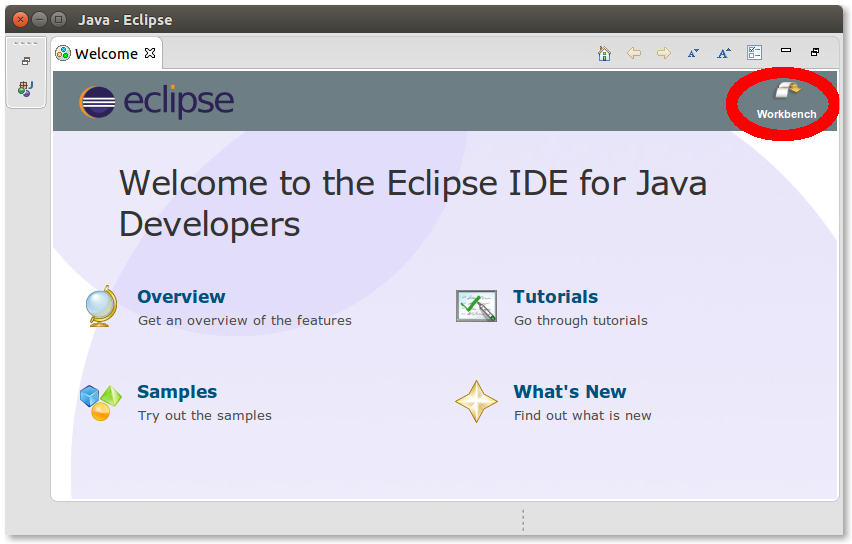
\includegraphics[width=1.0\textwidth]{../img/eclipse/eclipse-welcome.png}
\caption{Välkomstfliken för Eclipse, som nås via menyn \MenuArrow{Help}\Menu{Welcome}. Gå vidare genom att klicka på \textit{Workbench}.}
\label{fig:appendix:eclipse:welcome}
\end{figure}

\subsubsection{Välja perspektiv och visa olika vyer}

Eclipse-fönstret kan innehålla många underfönster i olika flikar, så kallade \textbf{views} eller vyer, som kan arrangeras på olika vis efter hur du vill ha dem. Vilka vyer som syns och hur de placeras beror på vilket s.k. \textbf{perspective} som är aktivt.  Figur \ref{fig:appendix:eclipse:open-perspective} visar arbetsytan med olika vyer i Java-perspektivet. 

Du kan byta till Scala-perspektivet genom att trycka på 
\includegraphics[scale=0.75]{../img/eclipse/eclipse-perspective-button.png} eller genom menyn \MenuArrow{Window}\MenuArrow{Perspective}\MenuArrow{Open Perspective}\MenuArrow{Other...}\Menu{Scala}.
Du kan anpassa inställningarna så att Scala blir \textit{default perspective}, se steg \ref{item:scala-perspective} i avsnitt \ref{subsection:appendix:ide:eclipse:tweaks} på sidan \pageref{subsection:appendix:ide:eclipse:tweaks}.

Stäng vyerna \textit{Task List} och \textit{Outline} om du vill ha mer plats till de övriga vyerna för paketnavigering, editering och utdata. Du kan öppna stängda vyer igen genom menyn \MenuArrow{Window}\Menu{Show View}. 

\begin{figure}
\centering
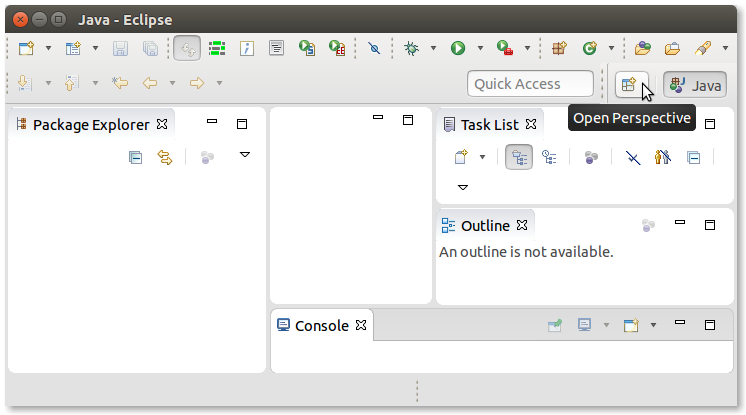
\includegraphics[width=1.0\textwidth]{../img/eclipse/eclipse-open-perspective.png}
\caption{Arbetsytan i Eclipse. Du kan växla mellan Scala- och Java-perspektivet genom att klicka på perspektivvalsknappen.}
\label{fig:appendix:eclipse:open-perspective}
\end{figure}

\subsubsection{Hello World}\label{subsubsection:eclipse:hello-world}

Efter att du öppnat Eclipse med ScalaIDE i ett tomt workspace och valt Scala-perspektivet enligt föregående avsnitt, kan du skapa ditt första projekt med ett \textit{''Hello World''}-program enligt stegen nedan.

\begin{enumerate}
\item Högerklicka i \Menu{Package Explorer} och välj \MenuArrow{New}\Menu{Scala Project}, varefter en dialogruta visas. 

\item Fyll i namnet \texttt{hello} i fältet \Menu{Project Name} och klicka \Button{Finish}.

\item Högerklicka igen i \Menu{Package Explorer} och välj \MenuArrow{New}\Menu{Scala Object}, varefter en ny dialogruta visas. 

\item Fyll i namnet \texttt{hi} i fältet \Menu{Project Name} och klicka \Button{Finish}.

\item Du får nu i editorvyn ett kodskellet med \code{object hi}.

\item Börja skriv \code{main} som visas i figur \ref{fig:appendix:eclipse:complete-main} och tryck Ctrl+Mellanslag för att aktivera kodkomplettering \Eng{code completion}. Då får du upp en lista med alternativ. Välj det översta alternativet \texttt{main} varefter ett kodskellet med en main-metod klistras in automatiskt i din kod.

\begin{figure}
\centering
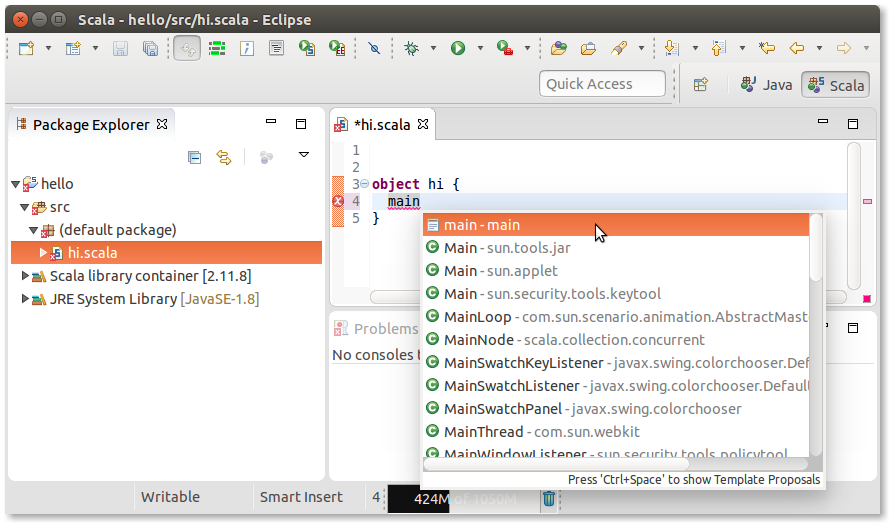
\includegraphics[width=1.0\textwidth]{../img/eclipse/eclipse-complete-main.png}
\caption{Aktivera kodkomplettering med Ctrl+Mellanslag efter ordet \code{main}.}
\label{fig:appendix:eclipse:complete-main}
\end{figure}

\item Fyll i lämplig utskriftstext i ett \code{println}-anrop så att din \code{main}-metod blir så som visas i editorfliken i figur \ref{fig:appendix:eclipse:hello-world}.

\begin{figure}[H]
\centering
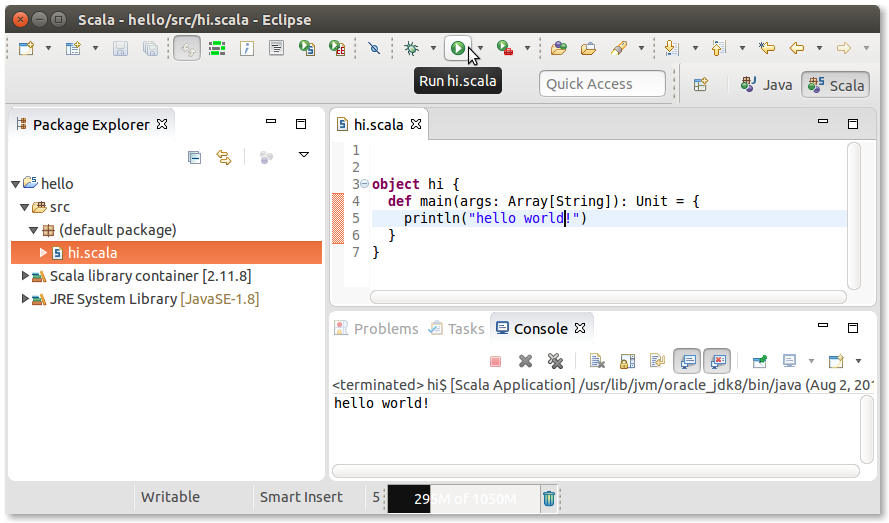
\includegraphics[width=1.0\textwidth]{../img/eclipse/eclipse-hello-world.png}
\caption{Skriv klart \code{main}-metoden och kör ditt program med play-knappen.}
\label{fig:appendix:eclipse:hello-world}
\end{figure}

\item Kör ditt program genom att trycka på den gröna play-knappen, som muspekaren i figur \ref{fig:appendix:eclipse:hello-world} pekar på. Du kan också trycka F11 för att köra igång din app, efter att du vid första körningen i dialogen \textit{Select Preferred Launcher} markerat  \FramedCheckmark{Use configuration specific settings} och valt alternativet \textit{Scala Application (new debugger) Launcher}. 

\end{enumerate}




\subsubsection{Ladda ner kursens workspace och importera i Eclipse}

Det finns en zip-fil med ett workspace med projekt för flera av kursens laborationer som du kan ladda ner och importera i Eclipse. Följ stegen nedan.

\begin{enumerate}
\item Ladda ner kursens workspace här: \url{http://cs.lth.se/pgk/ws}

\item Packa upp filen på lämpligt ställe.

\item Starta Eclipse med ScalaIDE-plugin (se startinstruktioner på sidan \pageref{subsubsection:start:eclipse}). 

\item Växla workspace till biblioteket du nyss packade upp, ungefär som i figur \ref{fig:eclipse:ide:open} och klicka \Button{OK}.

\begin{figure}[H]
\centering
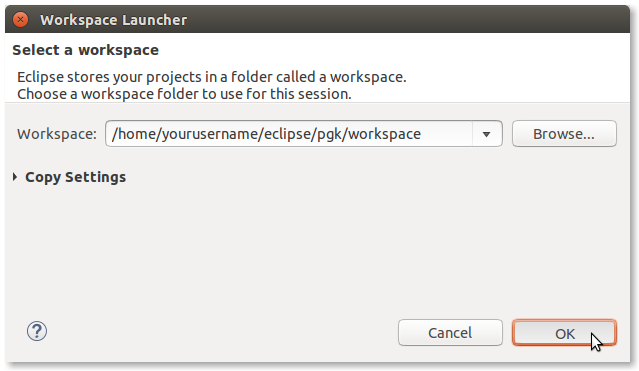
\includegraphics[width=1.0\textwidth]{../img/eclipse/eclipse-select-workspace.png}
\caption {Öppna kursens workspace genom att bläddra till biblioteket där du packade upp filen som du laddat ned från: \url{http://cs.lth.se/pgk/ws} }
\label{fig:eclipse:ide:open}
\end{figure}

\item Stäng välkomstfliken för att komma vidare till workbench (se figur \ref{fig:appendix:eclipse:welcome} på sidan \pageref{fig:appendix:eclipse:welcome}). Det ser då ut ungefär som i figur~\ref{fig:appendix:eclipse:open-perspective} på sidan \pageref{fig:appendix:eclipse:open-perspective}. Det syns ännu inget i \textit{Package Explorer} då vi ännu inte importerat något projekt. 

\item Innan du går vidare, säkerställ att du har Scala-perspektivet aktiverast. Du kan växla till Scala-perspektivet genom att trycka på 
\includegraphics[scale=0.75]{../img/eclipse/eclipse-perspective-button.png} eller genom menyn \MenuArrow{Window}\MenuArrow{Perspective}\MenuArrow{Open Perspective}\MenuArrow{Other...}\Menu{Scala}.
Du kan anpassa inställningarna så att Scala blir \textit{default perspective}, se steg \ref{item:scala-perspective} i avsnitt \ref{subsection:appendix:ide:eclipse:tweaks} på sidan \pageref{subsection:appendix:ide:eclipse:tweaks}.


\item Högerklicka i \textit{Package Explorer} och välj \Menu{Import...}, se Fig.~\ref{fig:eclipse:import}, eller välj menyn \MenuArrow{File}\Menu{Import...}. 

\begin{figure}[H]
\centering
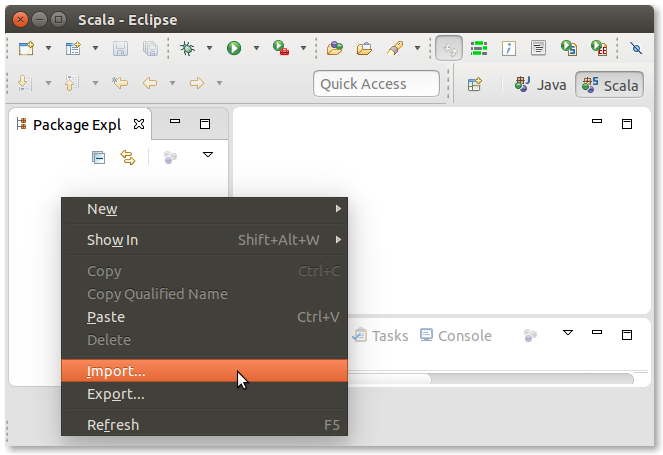
\includegraphics[width=1.0\textwidth]{../img/eclipse/eclipse-import.png} 
\caption {Välj \Menu{Import}-menyn för att importera existerande projekt.}
\label{fig:eclipse:import}
\end{figure}

\item Nu öppnas \Menu{Import}-dialogen som visas i figur \ref{fig:eclipse:import-existing}. Öppna mappen \Menu{General}, markera \textbf{Existing Projects into Workspace} och klicka \Button{Next}.



\begin{figure}[H]
\centering
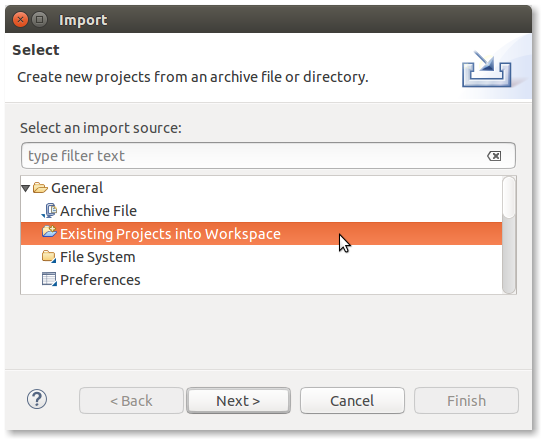
\includegraphics[width=0.75\textwidth]{../img/eclipse/eclipse-import-existing.png} 
\caption {Välj att importera existerande projekt under \Menu{General}.}
\label{fig:eclipse:import-existing}
\end{figure}


\begin{figure}[H]
\centering
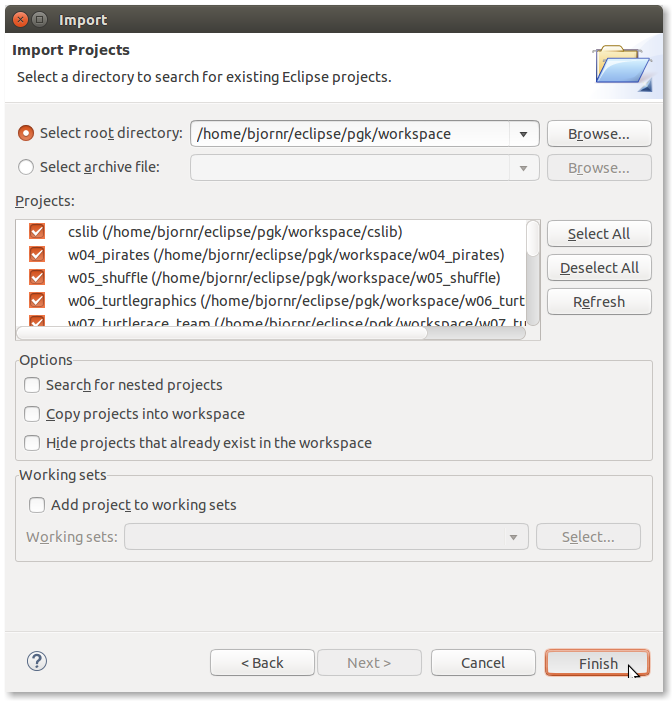
\includegraphics[width=1.0\textwidth]{../img/eclipse/eclipse-import-projects.png} 
\caption {Välj \FramedCheckmark{Select Root Directory} och klicka \Button{Browse}.}
\label{fig:eclipse:import-projects}
\end{figure}


\item Nu kommer ytterligare ett dialogfönster som visas i figure \ref{fig:eclipse:import-projects}. Med \FramedCheckmark{Select Root Directory} markerad kan du klicka \Button{Browse} för att ange workspace-mappen i ännu en dialog där du bara ska trycka \Button{Ok} utan att välja underbibliotek till workspace. När det är klart ska det se ut som i figur \ref{fig:eclipse:import-projects} där alla Eclipse-projekt \FramedCheckmark{cslib}, \FramedCheckmark{w04\_pirates}, etc. är markerade. Klicka sedan \Button{Finish}.

\item Följ ''Hello World''-instruktionerna på sidan \pageref{subsubsection:eclipse:hello-world} och skapa programmet som visas i figure \ref{fig:eclipse:pirates-hi}, genom att veckla ut projektet \textbf{w04\_pirates}, markera och högerklicka på paketet \textbf{priates}, och välja \MenuArrow{New}\Menu{Scala Object}.

\item Om du får problem, fråga någon som känner till Eclipse om hjälp. Det finns även mycket hjälp på nätet, se till exempel: \\ \href{http://stackoverflow.com/questions/8522149/eclipse-not-recognizing-scala-code}{stackoverflow.com/questions/8522149/eclipse-not-recognizing-scala-code}

\begin{figure}[H]
\centering
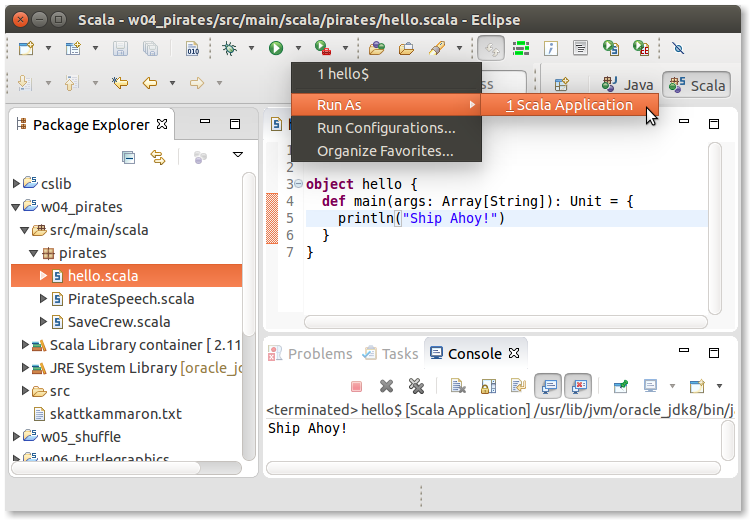
\includegraphics[width=1.0\textwidth]{../img/eclipse/eclipse-pirates-hello.png} 
\caption {Skapa ett \MenuArrow{New}\Menu{Scala Object} med kod enligt bilden.}
\label{fig:eclipse:pirates-hi}
\end{figure}


\end{enumerate}



\newpage

\section{IntelliJ IDEA}\label{appendix:ide:intellij}

IntelliJ IDEA%
\footnote{\href{https://en.wikipedia.org/wiki/IntelliJ_IDEA}{en.wikipedia.org/wiki/IntelliJ\_IDEA}}
 är en professionell IDE som stödjer många olika programmeringsspråk. IntelliJ är skriven i Java och utvecklas av det tjeckiska företaget JetBrains. 

IntelliJ IDEA finns i två varianter: en gratis gemenskapsvariant med öppenkällkodslicens \Eng{Community edition}, samt en betalvariant med sluten källkod och support-tjänster.


Till IntelliJ IDEA finns en insticksmodul \Eng{plug-in} som erbjuder stöd för Scala med tillhörande standardbibliotek..

IntelliJ IDEA är en omfattande och avancerad programmeringsmiljö med många funktioner och inställningar. Det finns även en omfattande uppsättning insticksmoduler och tilläggsprogram som underlättar utveckling av t.ex. webbprogram, databaser och mycket annat. 

I detta avsnitt ges länkar till installation samt tips om hur du kommer igång med att använda IntelliJ IDEA med Scala. Det går ganska snabbt att lära sig grunderna, men det kräven en viss ansträngning att lära sig de mer avancerade funktionerna. Det finns omfattande resurser på nätet som hjälper dig vidare. 

Google tillkännagav 2013 att företaget övergår från Eclipse till IntelliJ som den officiellt understödda utvecklingsmiljön för Android och 2014 lanserades utvecklingsmiljön AndroidStudio%
\footnote {\href{https://en.wikipedia.org/wiki/Android_Studio}{en.wikipedia.org/wiki/Android\_Studio}}
 som bygger vidare på IntelliJ. 

\subsection{Installera IntelliJ med Scala}\label{appendix:ide:intellij:install}

IntelliJ med Scala-plug-in är förinstallerat på LTH:s datorer och startas med kommandot \texttt{idea} i ett terminalfönster.

\begin{itemize}
\item För Ubuntu Linux finns ett färdigt paket som du kan installera med dessa kommandon i terminalen: 
\begin{REPLnonum}
sudo add-apt-repository ppa:mmk2410/intellij-idea-community
sudo apt-get update
\end{REPLnonum}
Mer information om denna ppa finns här:\\ \url{https://launchpad.net/~mmk2410/+archive/ubuntu/intellij-idea-community}\item För Windows och Mac: ladda ner och kör installationsfil för ditt operativsystem för den öppna varianten kallad \textbf{Community} här: \\
\url{https://www.jetbrains.com/idea/download/} \\
Följ instruktionerna som ges av installationsprogrammet.
\end{itemize}

\subsection{Anpassa IntelliJ}\label{appendix:ide:intellij:tweak}
Första gången du kör igång IntelliJ får du ett antal frågor om vilka anpassningar du vill göra. Följ instruktionerna steg för steg enligt nedan.
\begin{enumerate}
\item \textbf{UI Theme}. Denna dialog gäller utseende på gränssnittet. Det tema som kallas \textit{Dracula} är en populär variant med nedtonade färger anpassade för att vara skonsamma mot ögonen. Klicka \Button{Next} när du valt tema.

\item \textbf{Default plugins}. Denna dialog gäller inställningar av befintliga insticksmoduler. Dessa inställningar fungerar bra som de är. Klicka \Button{Next}.

\item \textbf{Featured plugins}. I rutan för \textbf{Plugin for Scala language support} Klicka \Button{Install} och låt installationen av Scala fullbordas. 

\item Klicka därefter \Button{Start using IntelliJ IDEA}.

\item I välkomstfönstrets nedre hörn, välj \MenuArrow{Configure}\Menu{Settings} och överväg om du vill göra följande lämpliga men ej nödvändiga inställningar. 
\begin{enumerate}
\item I fliken \MenuArrow{Editor}\Menu{General} markera \FramedCheckmark{Change font size (Zoom) with Ctrl+Mouse Wheel} för att lätt kunna ändra textstorlek i editorn. Klicka \Button{Apply} nere till höger.

\item I fliken \MenuArrow{Editor}\Menu{Inspections} och välj \Menu{Spelling} i högra listan. Avmarkera \FramedUnchecked{Typo} för att undvika att svenska ord blir markerade som felstavade. Klicka \Button{Apply} nere till höger.

\item I fliken \MenuArrow{Editor}\Menu{File and Code Templates} och under fliken \Menu{Files} i högra listan: för varje Scala-filtyp (Scala Class, Scala Trait, Scala Object, ...) ta bort de initiala raderna i mallen som börjar med \code{#} för att slippa onödiga kommentarer i koden när du skapar nya filer. Klicka \Button{Apply} nere till höger.
 
\end{enumerate} 
Du kan också göra ovan och liknande anpassningar senare genom menyn \MenuArrow{File}\Menu{Settings...}
\end{enumerate} 

\subsection{Använda IntelliJ}\label{appendix:ide:intellij:use}

\subsubsection{Skapa ett nytt projekt}

När du startar IntelliJ IDEA utan förvalt projekt visas välkomstskärmen i figur \ref{fig:idea:welcome}. Klicka på \Menu{Create New Project}, varefter dialogen i figur \ref{fig:idea:new-project} visas. Följ stegen enligt nedan.

\begin{figure}[H]
\centering
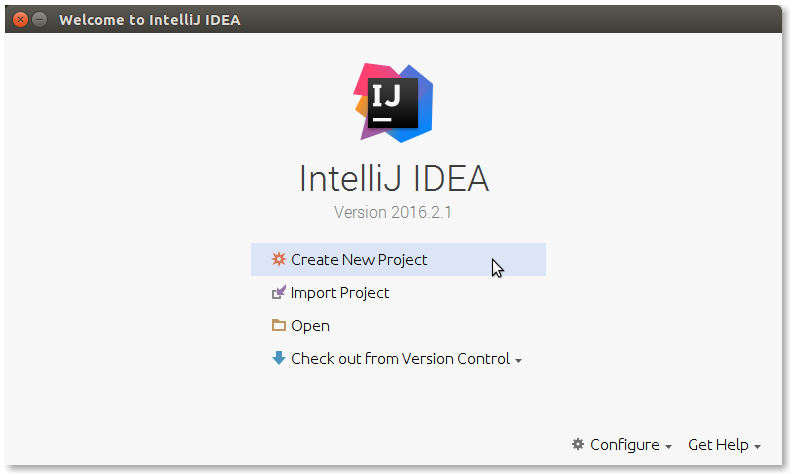
\includegraphics[width=0.8\textwidth]{../img/intellij/idea-welcome.png} 
\caption{Välkomstfönstret för IntelliJ IDEA.}
\label{fig:idea:welcome}
\end{figure}

\begin{enumerate}
\item I dialogen \textbf{New Project} ska du ge projektet ett namn och välja körmiljö för ditt projekt. Ge projektet namnet \texttt{hello} enligt figur \ref{fig:idea:new-project}. 

\item Välj sedan att skapa ett Scala-projekt genom att markera \textbf{Scala} enligt figur \ref{fig:idea:new-scala-project} och klicka \Button{Next}.

\begin{figure}[H]
\centering
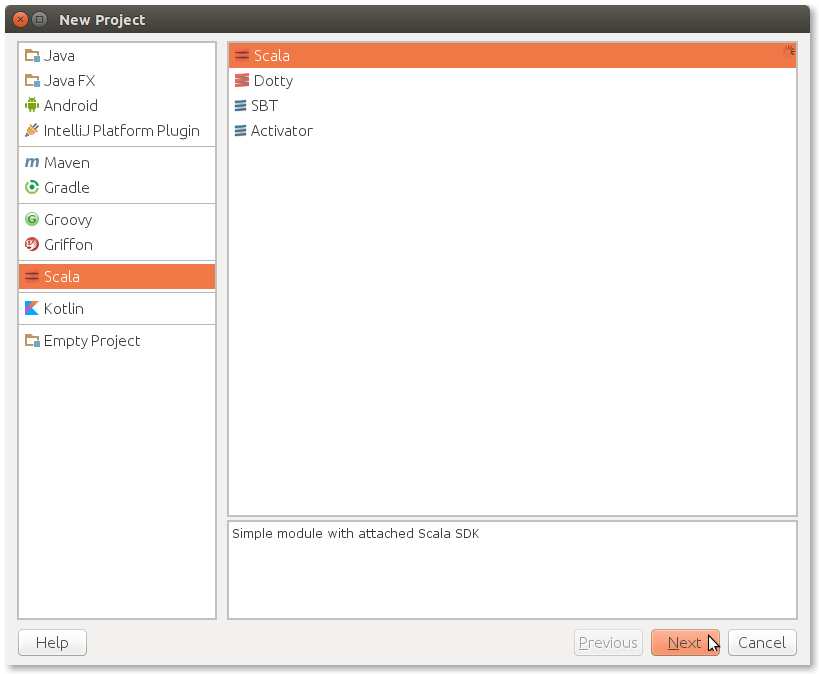
\includegraphics[width=0.65\textwidth]{../img/intellij/idea-new-scala-project.png} 
\caption{Välj att skapa ett Scala-projekt.}
\label{fig:idea:new-scala-project}
\end{figure}

\item Välj sedan \textbf{Project SDK} genom att klicka på \Button{New...}, välja \textit{JDK} och sedan veckla ut fliken \textit{JVM} och  välja \code{Oracle_jdk8} och klicka \Button{OK} enligt  figur \ref{fig:idea:new-project}.

\item Välj sedan \textbf{Scala SDK} genom att klicka på \Button{Create...}, markera raden med \textit{System 2.11.8} och klicka \Button{OK} enligt  figur \ref{fig:idea:new-project}.

\item Avsluta med att klicka \Button{Finish} i dialogen \textbf{New Project}.

\begin{figure}[H]
\centering
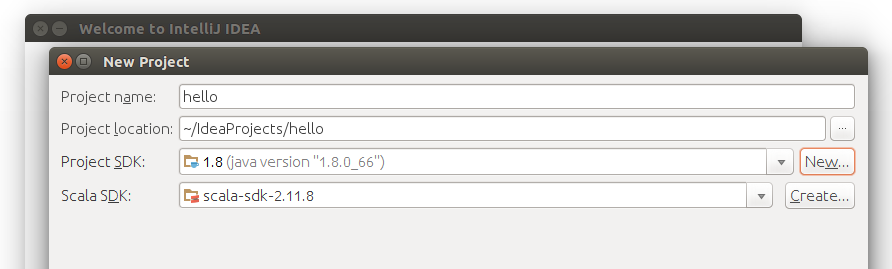
\includegraphics[width=1.0\textwidth]{../img/intellij/idea-new-project.png} 

\begin{minipage}{0.27\textwidth}
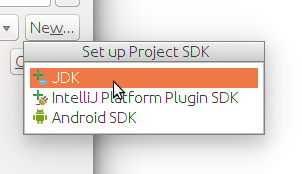
\includegraphics[width=1.0\textwidth]{../img/intellij/idea-project-sdk-jvm.png} 
\end{minipage}
\begin{minipage}{0.35\textwidth}
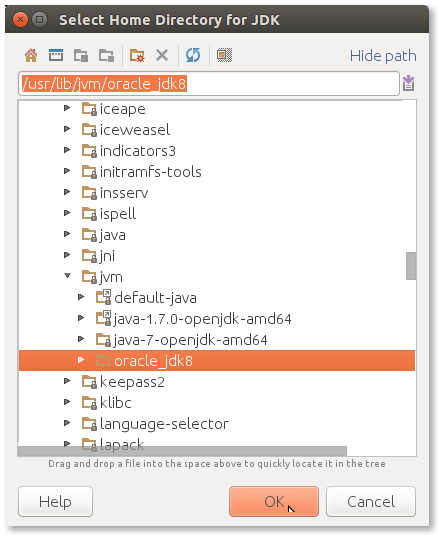
\includegraphics[width=1.0\textwidth]{../img/intellij/idea-project-sdk-home.png} 
\end{minipage}
\begin{minipage}{0.35\textwidth}
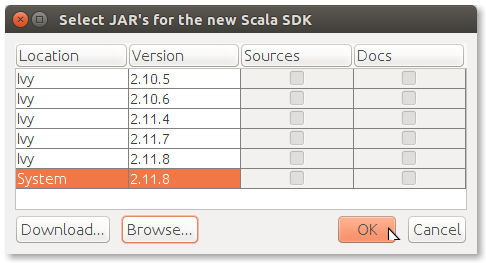
\includegraphics[width=1.0\textwidth]{../img/intellij/idea-scala-sdk.png} 
\end{minipage}%

\caption{Namnge ditt projekt och ställ in körmiljön för JVM och Scala genom att klicka på \Button{New...} och \Button{Create...}}.
\label{fig:idea:new-project}
\end{figure}

\item Du får nu ett projektfönster som liknar det i figur \ref{fig:idea:project-hello} på sidan \pageref{fig:idea:project-hello}.


\begin{figure}
\centering
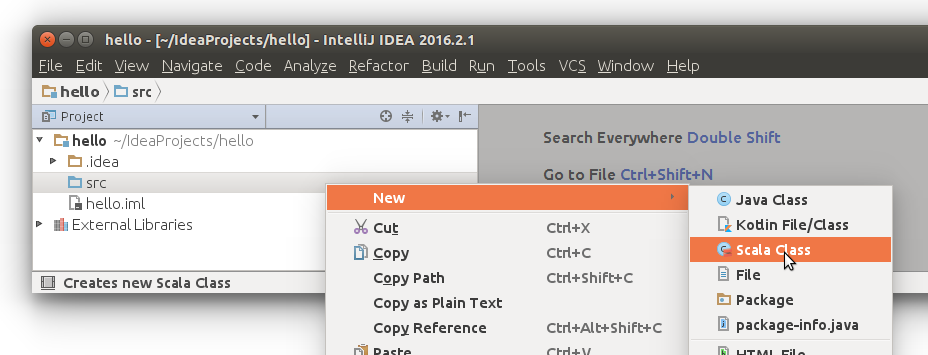
\includegraphics[width=1.0\textwidth]{../img/intellij/idea-new-scala-class.png} 

\begin{minipage}{0.35\textwidth}
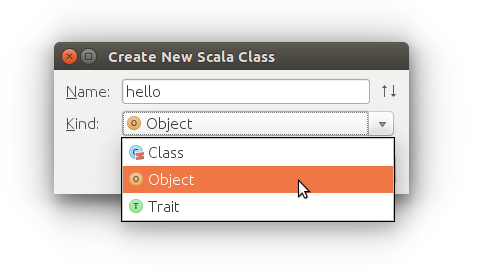
\includegraphics[width=1.0\textwidth]{../img/intellij/idea-scala-object.png} 
\end{minipage}
\begin{minipage}{0.60\textwidth}
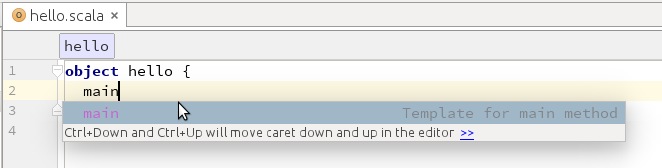
\includegraphics[width=1.0\textwidth]{../img/intellij/idea-complete-main.png} 
\end{minipage}%

\caption{Högerklicka på mappen \textbf{src} och välj \MenuArrow{New}\Menu{Scala Class} och skapa ett nytt Scala-objekt med main-metod. Aktivera kodkomplettering i editorn efter ordet main med TAB.}
\label{fig:idea:project-hello}
\end{figure}


\item Veckla ut ditt projekt och högerklicka på \texttt{src} och välj \MenuArrow{New}\Menu{Scala Class}.Välj sedan \textbf{Object} i dialogen \textbf{Create New Scala Class} och klicka \Button{OK}, enligt figur \ref{fig:idea:project-hello}.

\item Du får nu upp ett editorfönster med koden för objektet \code{hello}. Skriv ordet \code{main} inuti objektet och tryck TAB för att aktivera kodkomplettering. En mall för main-metoden klistras då in i objektet. 

\item Skriv kod så att det ser ut som i editorfönstret i figur \ref{fig:idea:hello-world} på sidan \pageref{fig:idea:hello-world}.

\item Kör igång ditt program genom att klicka på play-knappen eller genom att trycka Shift+F10. Om play-knappen är initialt är grå i stället för grön, välj menyn \MenuArrow{Run}\Menu{Run...}. 

\end{enumerate}


\noindent Mer information om hur du använder Scala-plugin för IntelliJ finns här:\\
\href{https://confluence.jetbrains.com/display/SCA/Scala+Plugin+for+IntelliJ+IDEA}{confluence.jetbrains.com/display/SCA/Scala+Plugin+for+IntelliJ+IDEA}

\begin{figure}
\centering
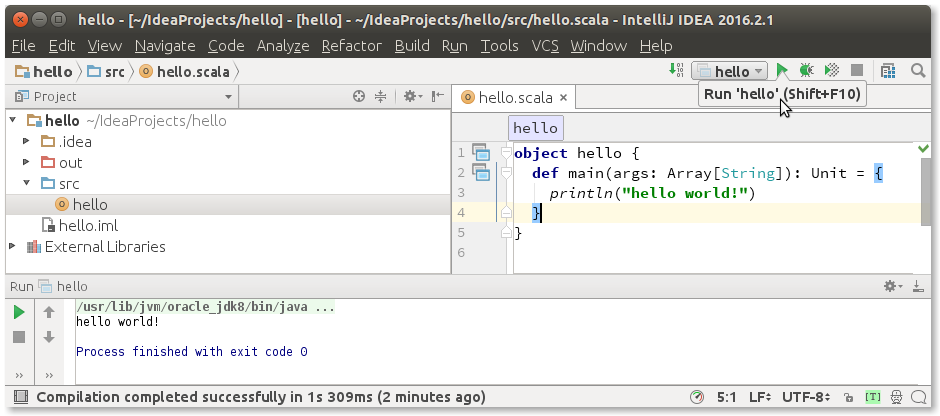
\includegraphics[width=1.0\textwidth]{../img/intellij/idea-hello.png} 
\caption{Kör ditt program med play-knappen eller \MenuArrow{Run}\Menu{Run...}.}
\label{fig:idea:hello-world}
\end{figure}


\subsubsection{Ladda ner kursens workspace och importera i IntelliJ IDEA}

Det finns en zip-fil med ett workspace med projekt för flera av kursens laborationer som du kan ladda ner och importera i Eclipse. Följ stegen nedan.

\begin{enumerate}
\item Ladda ner kursens workspace här: \url{http://cs.lth.se/pgk/ws}

\item Packa upp filen på lämpligt ställe.

\item Starta IntelliJ. Om du redan har ett projekt igång välj menyn \MenuArrow{File}\Menu{Close project} så kommer du tillbaka till välkomstfönstret. Välj \textbf{Import Project} så som visas i figure \ref{fig:idea:import1-project}.

\begin{figure}[H]
\centering
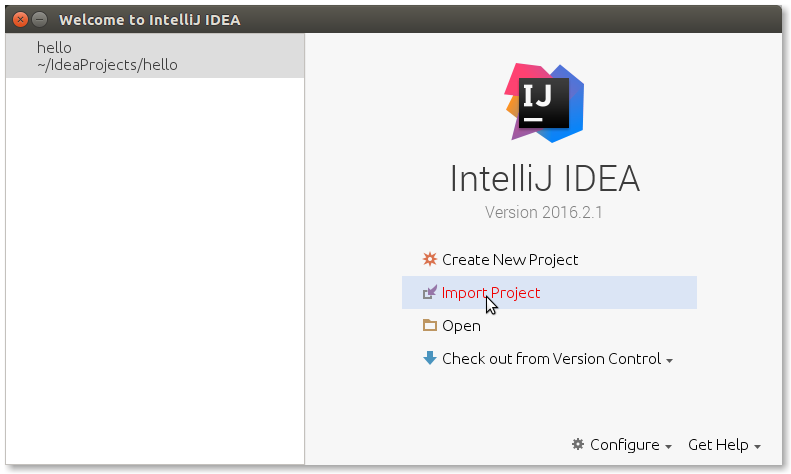
\includegraphics[width=1.0\textwidth]{../img/intellij/idea-import1-project.png} 
\caption{Välj \Menu{Import Project} efter att du stängt ev. öppna projekt.}
\label{fig:idea:import1-project}
\end{figure}

\item Bläddra dit du packat upp workspace och markera denna folder i likhet med figur \ref{fig:idea:import23-select} och klicka \Button{OK}. I den efterföljande dialogen välj \textbf{Eclipse} och klicka \Button{Next}.

\item Klicka \Button{Next} igen i dialogen som liknar figur \ref{fig:idea:import4-directory} på sidan \pageref{fig:idea:import4-directory}, där mappen du valt är förvald.

\item Klicka \Button{Next} igen enligt figur \ref{fig:idea:import5-select-projects} på sidan  \pageref{fig:idea:import5-select-projects}. Alla tillgängliga Eclipse-projekt ska vara markerade.

\item Klicka \Button{Finish} enligt figur \ref{fig:idea:import5-select-projects} med förifylld text oförändrad.

\item Bläddra fram filen \texttt{PirateSpeech.scala} och öppna den med ett dubbelklick. Klicka på länken \textbf{Setup Scala SDK} uppe till höger enligt figur \ref{fig:idea:import78-setup-scala-sdk} på sidan \pageref{fig:idea:import78-setup-scala-sdk}. I efterföljande dialog kontrollera att \texttt{scala-sdk-2.11.8} är förvalt och klicka \Button{OK}.

\item Lägg till testutskrift enligt rad 7 i figur \ref{fig:idea:import9-run} på sidan \pageref{fig:idea:import9-run}. Testkör genom att välja menyn \MenuArrow{Run}\Menu{Run..} eller tryck Alt+Shift+F10 och sedan välja \code{PirateSpeech}. Kontrollera att utskriften i utskriftsfönstret ser ut som förväntat.
\end{enumerate}

\noindent Om du får problem på vägen, be någon med erfarenhet av IntelliJ om hjälp.


{\vfill
\begin{figure}[H]
\centering
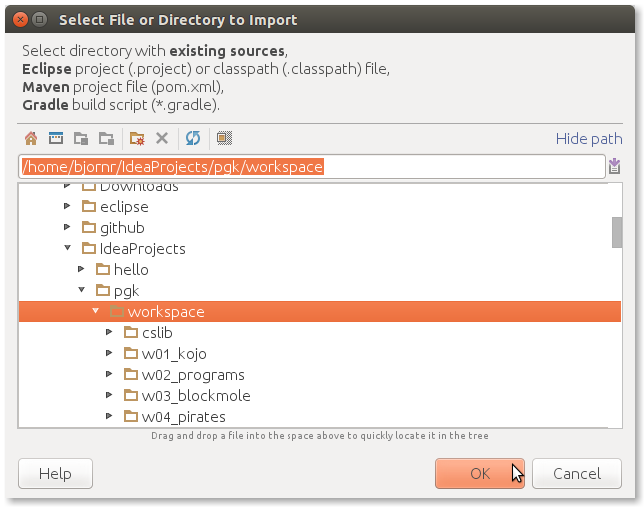
\includegraphics[width=1.0\textwidth]{../img/intellij/idea-import2-select.png} 

{\hfill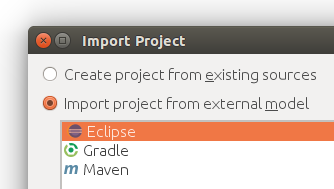
\includegraphics[width=0.4\textwidth]{../img/intellij/idea-import3-eclipse.png}} 

\caption{Markera den upp-packade workspace-mappen från zip-filen som du laddat ner från: \url{http://cs.lth.se/pgk/ws} och välj \textbf{Eclipse}-import.}
\label{fig:idea:import23-select}
\end{figure}
}

\begin{figure}
\centering
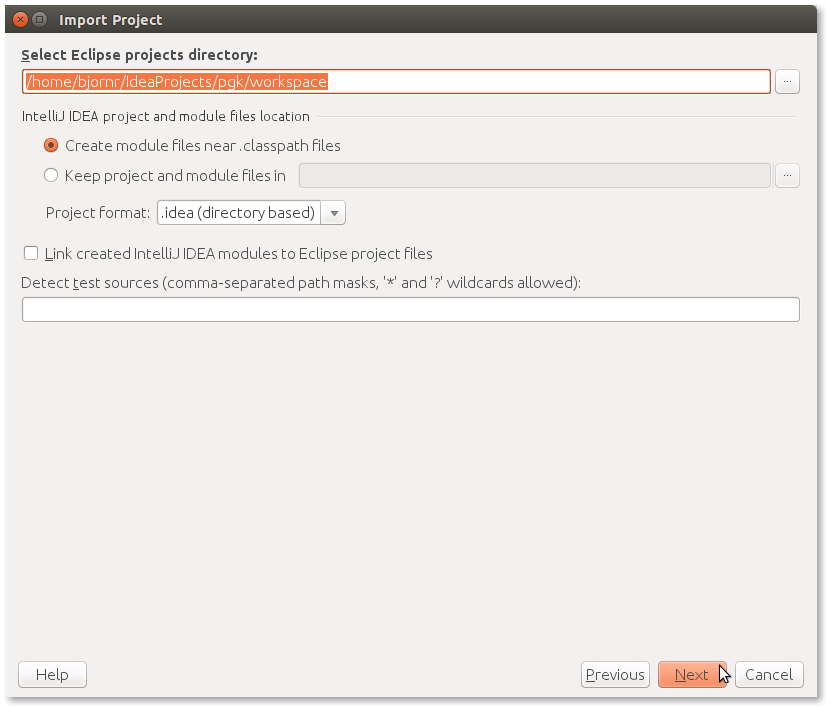
\includegraphics[width=0.85\textwidth]{../img/intellij/idea-import4-directory.png} 
\caption{Klicka \Button{Next} med förvalda alternativ oförändrade.}
\label{fig:idea:import4-directory}
\end{figure}

\begin{figure}
\centering
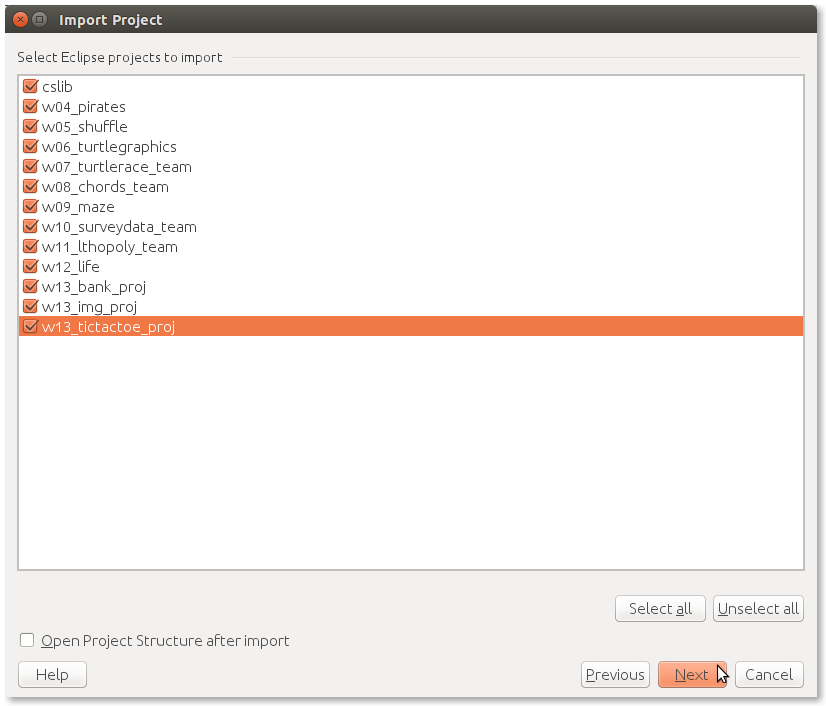
\includegraphics[width=0.85\textwidth]{../img/intellij/idea-import5-select-projects.png} 
\caption{Klicka \Button{Next} med alla projekt markerade.}
\label{fig:idea:import5-select-projects}
\end{figure}

\begin{figure}
\centering
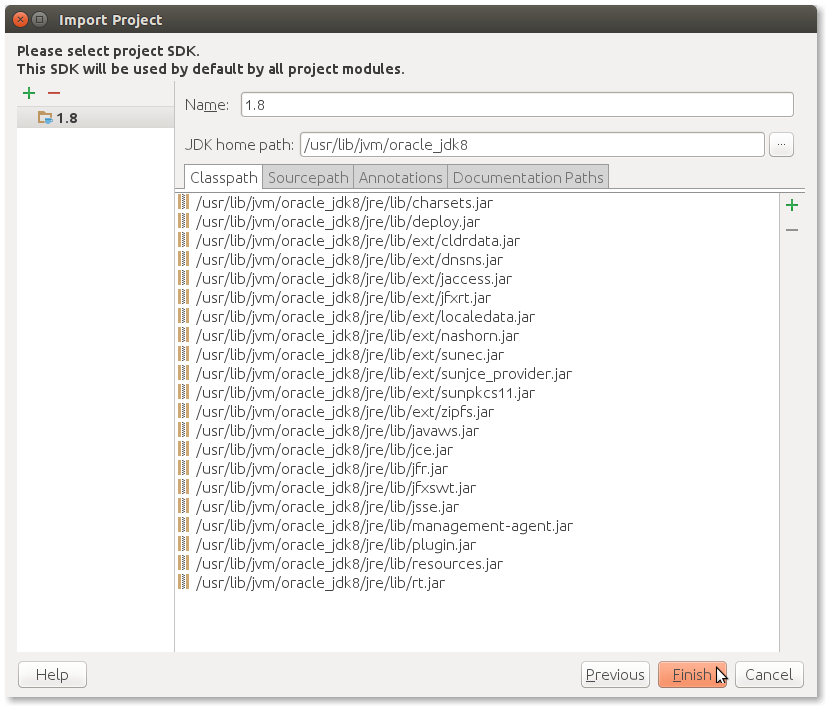
\includegraphics[width=0.8\textwidth]{../img/intellij/idea-import6-select-SDK.png} 
\caption{Klicka \Button{Finish} med förifyllda fält oförändrade.}
\label{fig:idea:import6-select-SDK}
\end{figure}

\begin{figure}
\centering
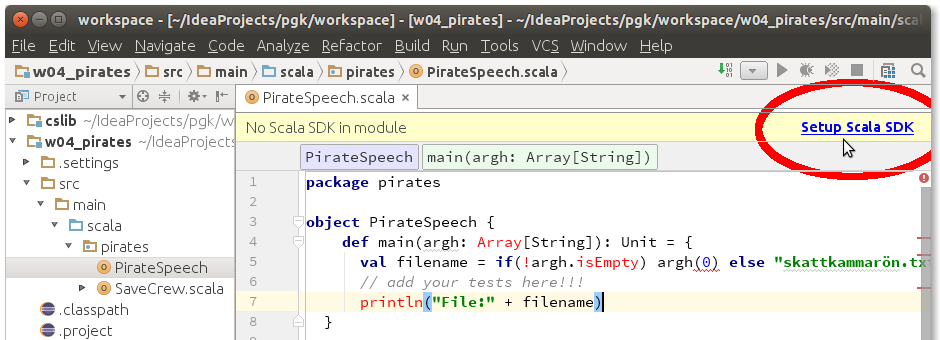
\includegraphics[width=1.0\textwidth]{../img/intellij/idea-import7-setup-scala-sdk.png} 

\vspace{1em}{\hfill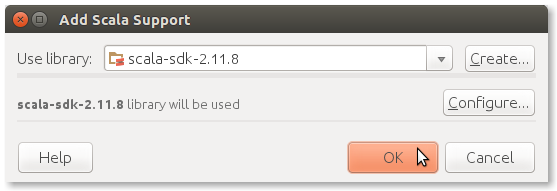
\includegraphics[width=0.6\textwidth]{../img/intellij/idea-import8-add-scala-support.png}} 
\caption{Bläddra fram PirateSpeech.scala i projektet \code{w04_pirates} och klicka på länken \textbf{Setup Scala SDK} och klicka \Button{OK} i efterföljande dialog.}
\label{fig:idea:import78-setup-scala-sdk}
\end{figure}

\begin{figure}
\centering
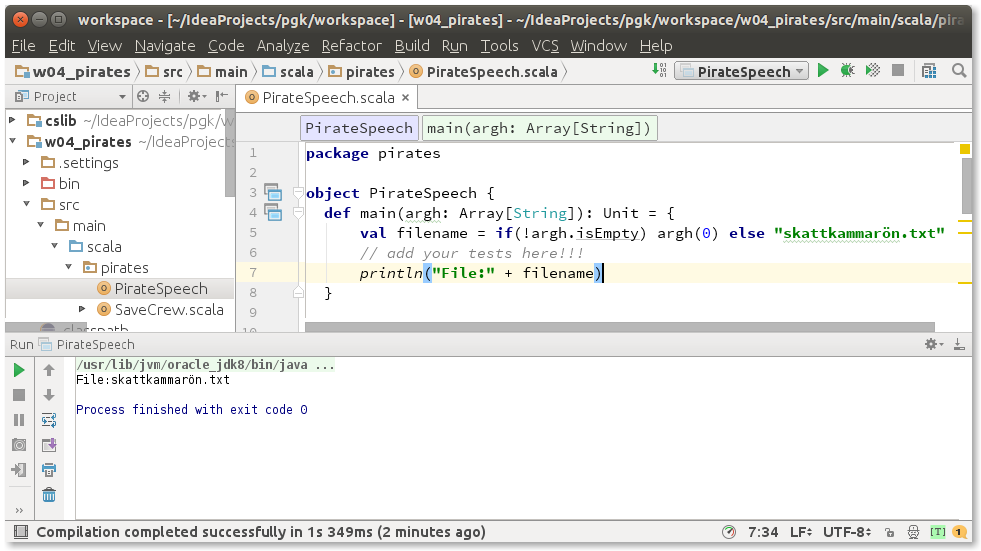
\includegraphics[width=1.0\textwidth]{../img/intellij/idea-import9-run.png} 
\caption{Lägg till utskriften i bilden ovan på rad7. Testkör genom att välja menyn \MenuArrow{Run}\Menu{Run..} (eller trycka Alt+Shift+F10) och sedan välja \code{PirateSpeech}. Observera utskriften i utskriftsfönstret.}
\label{fig:idea:import9-run}
\end{figure}





%!TEX encoding = UTF-8 Unicode
%!TEX root = ../compendium.tex

\chapter{Fixa buggar}\label{appendix:debug}

\begin{figure}[H]
\centering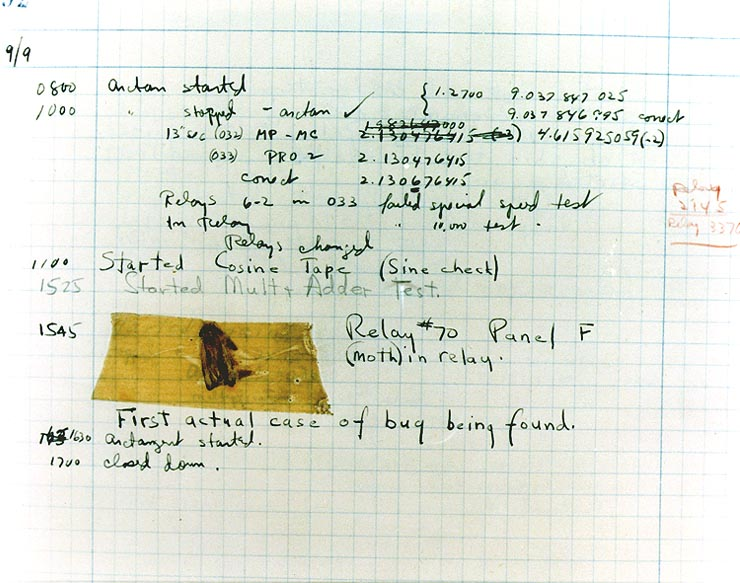
\includegraphics[width=0.85\textwidth]{../img/bug}

\caption{Den första dokumenterade buggen hittades 9 september 1947 i en Mark II Aiken Relay Calculator av Grace Hopper.\protect\footnotemark}

\end{figure}\footnotetext{\href{https://commons.wikimedia.org/w/index.php?curid=165211}{commons.wikimedia.org/w/index.php?curid=165211} Courtesy of the Naval Surface Warfare Center, Dahlgren, VA., 1988. - U.S. Naval Historical Center Online Library Photograph NH 96566-KN, Public Domain.   }


\section{Vad är en bugg?}

En bugg, även kallad lus \Eng{bug}, är en felaktighet som kan göra så att ett program inte beter sig som det är tänkt, och kan innebära oönskad utdata, att programmet kraschar, eller till och med ond bråd död.\footnote{\href{https://www.theguardian.com/technology/2016/jul/01/tesla-driver-killed-autopilot-self-driving-car-harry-potter}{www.theguardian.com/technology/2016/jul/01/tesla-driver-killed-autopilot-self-driving-car-harry-potter}}

Ursprunget till ordets användning i programmeringssammanhang är något oklar, men kan härledas till engelskans \emph{bug} som betyder insekt eller småkryp. 
Man brukar berätta att vid en felsökning av ett program som körde i en tidig dator byggd med  elektromekaniska reläer, uppdagades en död nattfjäril ihjälklämd mellan drivankaret och spolen i ett relä, som orsakade att programmet inte kunde exekveras korrekt. 



\subsection{Olika sorters fel}

När man ska lära sig mer om fel i programvarubaserade system, och hur de kan åtgärdas, är det viktigt att noga skilja på \textbf{misstag} \Eng{error}, \textbf{felorsak} \Eng{fault} och \textbf{felyttring} \Eng{failure}. 

Med ''misstag'' menar vi här ett fel som begås av människor (utvecklare, systemadministratörer, operatörer, användare, etc.) medan de skapar och använder ett programvarusystem. Det kan bli fel i olika delar av processen: 
\begin{itemize}
\item \textbf{Kravfel} uppstår medan man tänker ut vad systemet ska göra och då misstar sig angående  användarnas behov och önskemål.
\item \textbf{Designfel} uppkommer när man utformar systemets struktur på ett dåligt sätt.
\item \textbf{Implementationsfel} begås när man programmerar och skriver felaktiga kodrader. 
\item \textbf{Testfel} förekommer vid provkörning av systemet då testkoden är felaktig och därför ger falskt alarm om ''fel'', trots att beteendet egentligen är korrekt.  
\item \textbf{Operatörsfel} sker när systemet lämnas över till de, som ska installera och köra systemet i skarp produktion, och där systemdriften \Eng{operations, ''ops''} sköts på ett sätt som får problematiska konsekvenser.
\item \textbf{Användarfel} händer då användarna ger felaktig indata, eventuellt i strid med riktlinjerna för hur systemet ska användas, som system inte klarar att hantera korrekt, varpå mer eller mindre allvarliga felbeteenden hos systemet följer.
\end{itemize} 
I olika delar av utvecklingsprocessen kan alltså misstag begås som, antingen omedelbart, eller någon gång i framtiden, kan orsaka fel. Men det är inte säkert att ett fel någonsin kommer att märkas. Kanske kommer de felaktiga kodraderna, som \emph{skulle} kunna orsaka ett fel, aldrig att exekveras. Eller så kommer ingen användare att någonsin vilja använda systemet så som stipuleras av (onödiga) krav. Det är alltså först när fel \emph{yttrar} sig vid exekvering som misstag märks.

Fel kan också kategoriseras utifrån \emph{hur} de upptäcks i utvecklingsprocessen. Man brukar skilja på fel upptäckta vid granskning, kompileringsfel och exekveringsfel, som diskuteras nedan:
\begin{itemize}
\item Fel upptäckta vid \textbf{granskning}. Ett effektivt sätt att upptäcka fel är att människor noga läser igenom sin egen, och andras kod och försöker leta efter möjliga problem och brister. Man blir ofta ''hemmablind'' när det gäller ens egen kod. Därför kan någon annans, oberoende granskning med ''nya, friska'' ögon vara mycket fruktbar.  I samband med kodgranskning kan man med fördel försöka bedöma  huruvida koden är lätt att läsa, lätt att ändra i eller om koden har andra viktiga kvaliteter som har betydelse för den framtida utvecklingen av koden. Ofta hittar man vid granskning även enkla programmeringsmisstag, så som felaktiga villkor och loop-räknare som inte räknas upp på rätt sätt etc.
  
\item \textbf{Kompileringsfel} uppkommer under kompilering och upptäcks tack vare kontroller som sker av  kompilatorn. 

Vid kompileringsfel får man också ofta av kompilatorn reda på \emph{var} i koden det är fel och \emph{varför} det är fel, så att sökandet efter felorsaken och åtgärdandet av misstaget underlättas. Men ibland är felmeddelandet från kompilatorn missvisande och pekar på helt fel ställe i koden, så det gäller att inte alltid lita blint på det kompilatorn skriver. Dessutom är felmeddelanden från kompilatorn ofta uttryckta i termer av språkets syntaktiska och semantiska regler och det tar tid att lära sig tolka kompilatorers felmeddelanden. Att skapa kompilatorer som ger bra felmeddelande är ett svårt problem som studeras inom den datavetenskapliga disciplinen \textit{kompilatorteknik}, vilken du kan lära mer om i kurser på avancerad nivå.

Olika programmeringsspråk erbjuder olika stora möjligheter att göra kontroller vid kompileringstid. En kompilator för ett språk med ett avancerat typsystem, som till exempel Scala, ger förhållandevis stora möjligheter att identifiera fel redan under kompileringen, medan man med ett språk med ett svagare typsystem, till exempel Javascript, får förlita sig på prestandahämmande kontroller som kompilatorn genererar i maskinkoden eller som du själv väljer att lägga in i källkoden för säkerhets skull. 
  
\item \textbf{Exekveringsfel}, även kallat körtidsfel \Eng{runtime error}, sker medan programmet körs. Det kan kräva viss, specifik indata under specifika exekveringsomständigheter (en viss processor, en viss minnesstorlek, en viss nätverkskapacitet etc.) för att ett exekveringsfel ska yttra sig. När ett exekveringsfel väl yttrar sig, kan olika saker hända:

\begin{itemize}

\item \textbf{Exekveringen ger oönskat resultat.} Det är inte säkert att ett exekveringsfel avbryter exekveringen; det är vanligt att felet ''bara'' resulterar i inkorrekt utdata eller på annat sätt ger dålig kvalitet. För att upptäcka detta innan systemet sätts i drift, är det allmän praxis att man skriver noga uttänkta \textbf{testfall} och analyserar \textbf{testresultat} från exekveringen av  testfallen i detalj genom att undersöka utdata i jämförelse med önskat resultat eller med vad som anses vara en tillräckligt hög kvalitetsnivå.

\item \textbf{Exekveringen hänger sig} \Eng{hang}. Ibland yttrar sig fel genom att inget alls ser ut att hända under exekveringen, vilket kan beror på t.ex.:  
\begin{itemize}[nolistsep]
\item en \textbf{oändlig loop}, som aldrig blir färdig, 
\item att det går \textbf{väldigt långsamt} eftersom bearbetningen av indata tar orimligt lång tid,
\item att programmet \textbf{väntar på indata} som aldrig kommer,
\item att olika jämlöpande delar av programmet väntar på varandra så att ett \textbf{dödläge} \Eng{deadlock} uppstår. 
\end{itemize}

När exekveringen hänger sig och man inte orkar vänta längre på att något ska hända, är det bara att brutalt avbryta exekveringen genom något lämpligt kommando som erbjuds i din körmiljö.\footnote{\texttt{kill -9} $<$pid$>$, Ctrl+C, Ctrl+Shift+C, Ctrl+Z eller något annat beroende körmiljö.} I värsta fall får man stänga av strömmen.

\item \textbf{Exekveringen kraschar} \Eng{crach}. Ibland blir det ett plötsligt tvärstopp och exekveringen avbryts med ett körtidsfelmeddelande. Detta kan bero på t.ex.:
\begin{itemize}[nolistsep]
\item att \textbf{minnet är slut}, antingen är det parameterminnet för funktionsanrop \Eng{stack memory} som tagit slut eller så är minnet för allokering av objekt som skapas under programmets gång \Eng{heap memory} fullt,
 
\item misstaget att försöka referera en \textbf{null-referens} som inte refererar till något objekt, utan har värdet \code{null}, vilket resulterar i  \textit{null pointer exceeption},

\item att ett s.k. \textbf{undantag} har ''kastats'' \Eng{throw exception} genom att den som skrivit programmet medvetet kodat så att ett oönskat feltillstånd \emph{ska} orsaka en krasch, om inte undantaget ''fångas'' \Eng{catch} och hanteras av omgivande kod. 
\end{itemize}

När systemet kraschar får man en lista med den aktuella kedjan av funktionsanrop i en \textbf{stackspårning} \Eng{stack trace}. Man kan också begära en utskrift av hela innehållet i minnet vid kraschen \Eng{memory dump}, men en sådan kan vara svår att tolka.

\end{itemize}

\end{itemize}

När systemet ger oönskade resultat, hänger sig eller kraschar, får man försöka återskapa exekveringsfelet i en omkörning och, med hjälp av instrumentering eller en debugger, försöka lista ut vad som händer precis \emph{innan} exekveringsfelet uppstår, se  avsnitt \ref{section:debugging}.

I kursen \textit{Programvarutestning} \Eng{Software Testing} lär du dig mer om systematiska metoder för att testa system så att fel kan förebyggas, identifieras och åtgärdas.

\subsubsection{Bugg eller feature?} 

När ett (eventuellt) fel upptäcks, kan det vara på sin plats att först ställa sig några grundläggande  frågor:

\begin{itemize}
\item Är detta verkligen ett ''fel'' eller är det egentligen ett avsett beteende? Det är inte alltid självklart om det är en bugg eller en medvetet skapad systemegenskap/funktion \Eng{feature}.

\item Är det kanske testfallet som har felaktig testkod, medan koden som testas egentligen fungerar alldeles utmärkt? Sådan problem kan vara speciellt svåra att lösa, då man ofta letar på fel ställe efter orsaken.

\item Om problemet är av kvalitativ natur kan man fråga sig: Var går egentligen gränsen för ''fel''? Är detta bra nog givet vad det kostar att förbättra kvaliteten? Kvalitetskrav berör egenskaper hos ett program som kan uttryckas på en glidande skala, där något kan vara mer eller mindre \emph{bra} eller \emph{dåligt} ur olika synvinklar. Sådana krav leder ofta till viktiga men svåra avvägningsbeslut under design och implementation, och kan göra testningsresultaten svårbedömda.

Här är några exempel på kvalitetskrav:
\begin{itemize}
\item \textbf{Prestandakrav} \Eng{performance requirements} avser hur snabbt och effektivt programmet ska arbeta under olika omständigheter.
 
\item \textbf{Kapacitetskrav} \Eng{capacity requirements} avser hur mycket data systemet ska klara av under olika omständigheter.

\item \textbf{Användbarhetskrav}\footnote{\href{https://sv.wikipedia.org/wiki/Anv\%C3\%A4ndbarhet}{sv.wikipedia.org/wiki/Användbarhet}} \Eng{usability requirements} avser krav på hur lättanvänt systemet ska vara för en given användarkategori. 
\end{itemize} 

\end{itemize}

I kursen \textit{Kravhantering} \Eng{Sofware Requirements Engineering} lär du dig mer om att identifiera, specificera och följa upp kvalitetskrav.

\subsubsection{Felärendehanteringsverktyg} 

Det är allmän praxis i industriell systemutveckling att använda sig av ett felärendehanteringsverktyg \Eng{issue tracker} så att samarbetande utvecklare får stöd i att hålla reda på alla uppkomna fel och problem \Eng{issue}. Många av de populära kodlagringsplatserna som finns på nätet, så som GitLab, GitHub och BitBucket (se avsnitt \ref{section:code-hosting}), erbjuder felärendehanteringsfunktioner. Dessa kan till exempel vara:
\begin{itemize}
\item hantering och sammanställning av alla olika ärendetillstånd, så att man kan se vilka issues som är i tillstånden \textit{Open} eller \textit{Closed},
\item tillording av ärende till specifika personer som ska åtgärda problemet,
\item gradering av ärende i olika allvarlighetsgrader,
\item meddelandegenerering till inblandade personer när ett ärende kommenteras eller ändrar tillstånd.
\end{itemize}


\section{Att förebygga fel}

Även om det nästan är oundvikligt att inte låta buggar slinka in i koden allteftersom den blir mer och mer komplex, är det ändå viktigt att lägga stor möda vid att försöka undvika att så sker. Det är ofta mycket bättre investerad tid att jobba med buggförebyggande åtgärder medan du skapar koden, än att jaga buggar som skulle ha kunna undvikas med allmän noggrannhet och stramare disciplin i kodningen. Nedan sammanfattas några åtgärder som är A och O för att minska mängden fel.

\begin{itemize}
\item \textbf{Skapa begriplig kod}. 
\item \textbf{Tänk ut bra namn}.
\item \textbf{Kontrollera villkor}.
\item \textbf{Lägg in typkontroller}. Typannoteringar möjliggör för kompilatorn att kontrollera dina hypoteser om vad koden gör.
\item \textbf{Hantera saknade värden}.
\item \textbf{Hantera undantag}.
\item \textbf{Granska kod}.
\item \textbf{Testa kod}.
\end{itemize}


\section{Vad är debugging?}

När en felyttring identifierats, t.ex. genom testning eller slutanvändare rapporterar om problem, vidtar sökandet efter den bakomliggande felorsaken, så att vi förstår \emph{varför} det blev fel och sedan kan \emph{åtgärda} misstaget. Denna process kallas \textbf{avlusning} \Eng{debugging}.




\subsection{Hur hitta felorsaken?}

Första steget i avlusningsprocessen är att hitta den bakomliggande felorsaken. Detta kan vara mycket svårt, speciellt om systemet är stort och komplicerat.

När du stirrar dig blind på koden utan att hitta felorsaken, kan det bero på att du har en felaktig hypotes om vad koden egentligen gör. Du är övertygad om att en viss sak händer, men \emph{egentligen} är det \emph{inte} det du \emph{tror} händer som \emph{verkligen} händer. Exempelvis kanske du antar att en räknare räknas upp i en loop, men i själva verket saknas uppräkningen. Om du oreflekterat accepterar ditt felaktiga antagande, är det stor risk att du letar på fel ställe i koden.

En grundläggande princip vid felsökning är att uttryckligen \emph{formulera hypoteser} som du har om vad som sker i systemet och sedan \emph{verifiera} att de verkligen stämmer, genom olika undersökningar av det exekverande systemet. Du ska alltså tydligt beskriva hur du tror att koden fungerar och sedan med olika former av instrumentering, t.ex. genom utskrifter i terminalen av variablers värden, kontrollera att så verkligen är fallet.

\subsubsection{Återskapa buggen med ett minimalt testfall}

\TODO

\subsubsection{Instrumentering med utskrifter, ''print-debugging''}

\TODO

Du kan även använda en avlusare \Eng{debugger}, som normalt ingår i en integrerad utvecklingsmiljö, för att instrumentera din kod. Se vidare i avsnitt \ref{section:debugging} om hur du använder avlusarna i Eclipse och IntelliJ IDEA.


\section{Åtgärda fel}

Ofta är det det svåraste att \emph{hitta} buggen, medan själva buggrättningen visar sig trivial. Har du, till exempel, väl hittat den saknade uppräkningen av din loop-variabel är det uppenbart vad du ska göra.

Men ibland är det riktigt knepigt att åtgärda felet. Nedan sammanfattas några av de situationer som kan uppkomma, som gör att felrättningen blir extra svår. 

\begin{itemize}
\item Kanske är själva algoritmen i grunden feltänkt och en helt ny algoritm behöver konstrueras. Att skapa nya algoritmer från grunden kan visa sig mycket svårt i en del fall. I fortsättningskurser får du lära dig mer om algoritmkonstruktionens ädla konst.

\item Kanske algoritmen fungerar för olika normalfall, medan ovanliga undantagsfall inte hanteras korrekt. Att på ett bra sätt hantera alla upptänkliga fall kan visa sig väldigt knepigt. Tyvärr är det ofta undantagsfall i kombination med buggar som öppnar för säkerhetsluckor redo att utnyttjas av elaka hackare för att krascha systemet eller smitta ner det med virus.

\item Kanske är problemet i sig väldigt svårt att lösa på ett korrekt sätt. Algoritmen kan vara riktigt knepig med många villkor, loopar och nästlade datastrukturer. Blir det fel i en sådan algoritm kan det ta lång tid att få ändringar att fungera och alla villkor, loopar och nästlade datastrukturer att passa ihop igen efter felrättningen. 

\item Medan man rättar en bug kan man råka att, av misstag, skapa nya buggar. Risken för detta är speciellt stor om koden är komplex. Ibland låter man till och med bli att åtgärda ett fel om systemet ändå fungerar hjälpligt i andra avseenden och risken är för stor att nya buggar skapas. Då behöver systemet strukturerats om så att det blir lättare att ändra i.

\item Kanske växer exekveringstiden exponentiellt med datamängden. Det kan då i praktiken vara omöjligt att skriva ett program som i alla lägen blir färdigt inom rimlig tid. Då får man försöka tänka ut kluriga genvägar till suboptimala lösningar som ändå duger, vilket ibland kräver mycket avancerad programmeringsteknik.
 
\end{itemize}

Det finns ingen allenarådande snabbfix att ta till när man stöter på svåra fel. Att bli en produktiv och kvalificerad systemutvecklare, som framgångsrikt reder ut allehanda buggar, handlar i stor utsträckning om att kombinera en bred allmänbildning inom datavetenskap med ett livslångt lärande, där varje bugg du hittar och åtgärdar ger dig nya kunskaper och erfarenheter inför framtiden.
\emph{Se varje bugg som en ny chans till ökad lärdom!}



\section{Använda en debugger}\label{section:debugging}

\begin{itemize}
\item \textbf{Sätta brytpunkter}.
\item \textbf{Stegad exekvering}.
\item \textbf{Inspektera variabler}.
\end{itemize}

\subsection{Debuggern i Eclipse med ScalaIDE}
\subsubsection{Sätta brytpunkter i Eclipse}\TODO
\subsubsection{Stegad exekvering i Eclipse}\TODO
\subsubsection{Inspektera variabler i Eclipse}\TODO

\subsection{Debuggern i IntelliJ IDEA med Scala-plugin}
\subsubsection{Sätta brytpunkter i IntelliJ}\TODO
\subsubsection{Stegad exekvering i IntelliJ}\TODO
\subsubsection{Inspektera variabler i IntelliJ}\TODO
%!TEX encoding = UTF-8 Unicode
%!TEX root = ../compendium.tex

\chapter{Dokumentation}\label{appendix:doc}

Dokumentation hjälper andra att använda din kod, men underlättar även för dig själv när du vid ett senare tillfälle ska erinra dig hur den fungerar och hur du ska använda och bygga vidare på din kod. Modern systemutveckling baseras ofta på öppen källkod och färdiga api \Eng{application programming interface}, där kvaliteten på dokumentationen är avgörande för hur lätt det är att komma igång med att använda koden.

Nedan listas exempel på olika typer av  dokumentation\footnote{\href{https://en.wikipedia.org/wiki/Software_documentation}{en.wikipedia.org/wiki/Software\_documentation}}:

\begin{itemize}
\item \textbf{Kravdokumentation} beskriver det övergripande målet med mjukvaran, samt funktionella krav och kvalitetskrav som uppfylls av systemet.
\item \textbf{Designdokumentation} beskriver arkitekturen, hur koden är organiserad i moduler, och den interna systemstrukturen t.ex. i form av klasser, objekt och deras relation.
\item \textbf{Slutanvändardokumentation} kan t.ex. vara manualer för användning av systemet och installationsanvisningar.
\item \textbf{Teknisk dokumentation} kan t.ex. vara api-dokumentation som beskriver vilka funktioner som ingår i ett programbibliotek. Sådan dokumentation genereras ofta med hjälp av ett \textbf{dokumentationsverktyg} (se avsnitt \ref{appendix:buildtool}).  Andra typer av teknisk dokumentation är instruktioner om hur man bygger koden med eventuellt tillhörande byggverktygskonfigurationsfiler; ofta beskrivs byggförfarandet steg för steg i en textfil med namnet \code{README}. (Läs mer om byggverktyg i appendix \ref{appendix:build}.) 
\end{itemize}

\noindent Det är en stor utmaning att hålla dokumentationen uppdaterad allteftersom koden utvecklas. Även om man får hjälp att generera en navigerbar sajt av ett dokumentationsverktyg, måste själva \textit{innehållet} i de manuellt författade dokumentationskommentarerna vara i överensstämmelse med den aktuella versionen av koden. Uppdateras koden, måste man alltså vara noga med att uppdatera dokumentationskommentarerna, annars uppstår stor förvirring. 

Detta problem är så pass allvarligt att man ska tänka sig noga för hur man kan formulera  dokumentationskommentarerna på ett framtidssäkert sätt, och hur omfattande de ska vara i förhållande till den framtida arbetsinsatsen med att hålla dem uppdaterade. Desto mer omfattande kommentarer desto mer jobb att hålla dem uppdaterade. 

Det är i praktiken svårt att uppnå en optimal balans mellan bra och många kommentarer som \textit{hjälper} användaren, och å andra sidan svårunderhållna och föråldrade kommentarer som \textit{stjälper} användare.


\section{Vad gör ett dokumentationsverktyg?}\label{appendix:buildtool}

Ett dokumentationsverktyg genererar teknisk dokumentation av koden baserat på speciella \textbf{dokumentationskommentarer} som skrivs i koden omedelbart före deklarationer av det som ska dokumenteras. Dessa dokumentationskommentarer skrivs enligt en speciell syntax som dokumentationsverktyget kan tolka.

Utdata från ett dokumentationsverktyg utgörs typiskt av en webbsajt med ändamålsenlig formatering och navigationslänkar, se figur \ref{fig:appendix:doctool}.

\begin{figure}[H]
\centering
\begin{tikzpicture}[node distance=1.8cm, scale=1.5]
\node (input) [startstop] {\bf\sffamily Källkod};
\node(inptext) [right of=input, text width=6cm, xshift=4.2cm]{med speciella dokumentationskommentarer före deklarationer};
\node (compile) [process, below of=input] {\bf\sffamily Dokumentationsverktyg};
%\node(explain) [right of=compile, text width=5cm, xshift=3.0cm]{Översätter från källkod till maskinkod};
\node (output) [startstop, below of=compile] {\bf\sffamily Dokumentation};
\node(outtext) [right of=output, text width=6cm, xshift=4.2cm]{t.ex. en webbsajt med dokumentation och navigationslänkar};
\draw [arrow] (input) -- (compile);
\draw [arrow] (compile) -- (output);
\end{tikzpicture}
    \caption{Ett dokumentationsverktyg läser koden och dokumentationskommentarer och genererar dokumentation, t.ex. i form av en webbsajt.}
    \label{fig:appendix:doctool}
\end{figure}



\section{scaladoc}
\newcommand{\scaladoc}{\texttt{scaladoc}}

Med Scala-installationen följer dokumentationsverktyget \scaladoc, som genererar en webbsajt med ändamålsenlig layout och specialfunktioner för att söka, filtrera och navigera i dokumentationen. 

Dokumentationen av stora bibliotek kan bli omfattande och det krävs träning i att använda dokumentationssajter för att få maximal nytta av dem. I efterföljande avsnitt beskrivs först hur du använder dokumentation som är genererad med \scaladoc. Därefter visas hur du själv kan generera dokumentation för din egen kod.


\subsection{Använda dokumentation från scaladoc}

Dokumentationen av Scalas standardbiliotek är genererad med \scaladoc~och att navigera i denna ger bra träning i hur man använder avancerad api-dokumentation. Du hittar dokumentationen för Scalas standardbibliotek här: \\
\url{http://scala-lang.org/api/current} 


När du surfar dit möts du av dokumentationen för \textit{root package}, som ger en översikt av olika paket i standardbiblioteket. I sökrutan uppe till vänster kan du skriva början på namnet på klasser, traits, eller objekt som du letar efter, så som visas i figure \ref{fig:scaladoc:root-package}.

\begin{figure}[H]
\centering
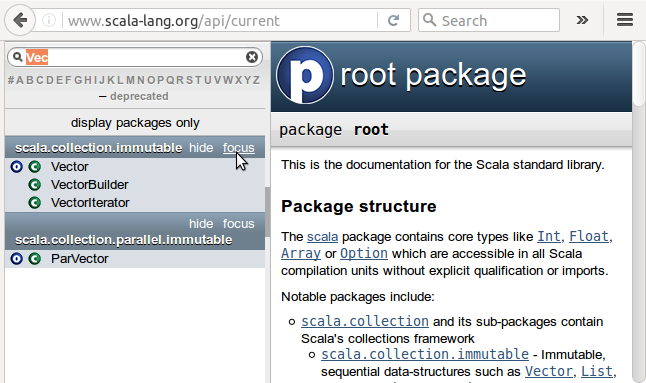
\includegraphics[width=0.8\textwidth]{../img/scaladoc/scaladoc-root}

     \caption{ \scaladoc.}
    \label{fig:scaladoc:root-package}
\end{figure}

Om du är speciellt intresserad av, t.ex., paketet \code{scala.collection.immutable}, kan du klicka \textbf{focus} för att begränsas visningen till att endast innehålla typerna i detta paket.

Om du söker efter typen där en viss metod är implementerad, men inte vet riktigt i vilken klass den finns, kan du klicka på bokstaven som metodnamnet börjar på i listan med bokstäver under den övre vänstra sökrutan. Då får du en lista med allt möjligt som börjar på F, så som visas i figur \ref{fig:scaladoc:find}. Sök i listan med din webbläsares sökfunktion (Ctrl+F) efter ''fill'', så hittar du alla typer som implementerar metoden \code{fill}. 

\begin{figure}[H]
\centering
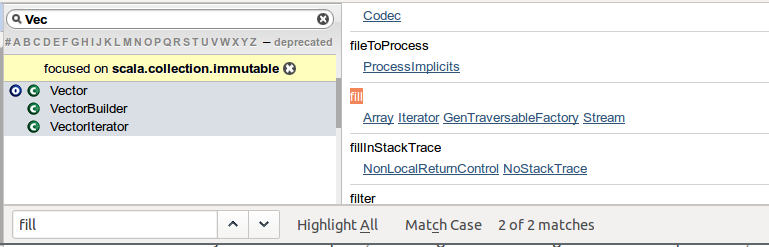
\includegraphics[width=1.0\textwidth]{../img/scaladoc/scaladoc-find-fill}

     \caption{ \scaladoc.}
    \label{fig:scaladoc:find}
\end{figure}

Om du klickar vidare, i detta exempel på länken till klassen Array, kan du sedan klicka på länken till källkoden i \texttt{array.scala} för att se implementationen på GitHub; sök på sidan med din webbläsares sökfunktion Ctrl+F efter ''def fill''.





Om du klickar på den typ du är intresserad av, t.ex. klassen Vector, får du upp en sida med en mängd information, inklusive alla metoder, även ärvda. Figur \ref{fig:scaladoc:vector} visar hur en sökning bland alla metoder i Vector initieras i sökrutan nere till höger, vilken kommer att visa metoder som börjar på ''rev'', här skrollas fönstret till metoden \code{reverse} längre ner på sidan.

Genom att klicka på det den gröna cirkeln med bokstaven C överst i dokumentationsfönstret, växlar du till vyn för kompanjonsobjektet där du hittar alla fabriksmetoder för Vector, även ärvda, t.ex. \code{fill} som du kan söka efter i sökrutan. 



\begin{figure}[H]
\centering
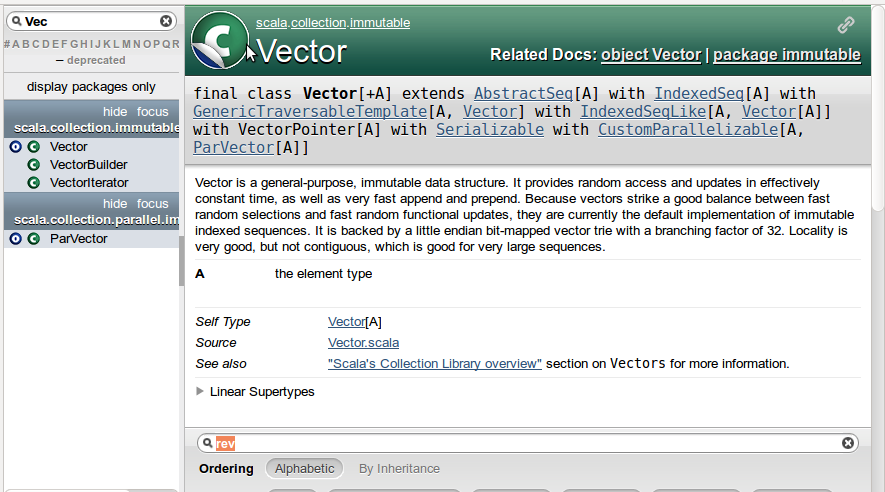
\includegraphics[width=1.0\textwidth]{../img/scaladoc/scaladoc-vec}

     \caption{ \scaladoc.}
    \label{fig:scaladoc:vector}
\end{figure}


\subsection{Skriva dokumentationskommentarer för scaladoc}


Verktyget \scaladoc~läser kommentarer som börjar med \verb|/**| och slutar med \verb|*/| och associeras till efterföljande deklaration. Notera de dubbla asteriskerna. Alla rader som följer efter \verb|/**| ska, enligt konventionen för Scalas dokumentationskommentarer, börja med en asterisk \code|*| med indrag med flera blanksteg så att den hamnar under \textit{andra} asterisken i öppningskommentaren, som nedan:
\begin{Code}
/** Först kommer en sammanfattning på en enda rad. 
  * 
  * Sedan kommer eventuellt en mer detaljerad beskrivning, 
  * som kan vara flera rader lång.
  */
\end{Code}
Dokumentationskommentaren slutar med \code|*/| rakt under asterisk-kolumnen.

I figur \ref{fig:scaladoc:mio} på sidan \pageref{fig:scaladoc:mio} visas exempel på dokumentationskommentarer. Annoteringen \verb|@param| i början på en rad ger en speciell kommentar angående parametrar. Annoteringen \verb|@return| i början av en rad ger en speciell kommentar angående vad som returneras vid metodanrop.


\subsection{Generera dokumentation med scaladoc}


Du genererar en dokumentationssajt med terminalkommandot \scaladoc~följt av en eller flera källkodsfiler. Med optionen \code{-d} anger du i vilket bibliotek sajten ska sparas. Du visar sajten genom att öppna filen \code{index.html} i en webbläsare. Nedan visas hur dokumentationen genereras för källkodsfilen i figur \ref{fig:scaladoc:mio}.
\begin{REPLnonum}
$ scaladoc mio.scala -d apidoc
$ firefox apidoc/index.html
\end{REPLnonum}

I figur \ref{fig:scaladoc:webpage} på sidan \pageref{fig:scaladoc:webpage} visas delar av en webbsida som genererats utifrån koden i figur \ref{fig:scaladoc:mio} på sidan \pageref{fig:scaladoc:mio}. För de publika metoder där ingen dokumentationskommentar finns, visas ändå metodens signatur med parametrar, parametertyper, och returtyp. Medlemmar som deklareras \code{private} visas inte, men om man klickar på knappen \Button{All} bredvid rubriken \textbf{Visibility} visas medlemmar som är deklarerade \code {protected}.

Om du klickar på symbolen \Forward~till vänster om metodsignaturen, ändras den till symbolen \MoveDown  ~som indikerar att den mer detaljerade beskrivningen av parametrar etc. har vecklats ut (i den mån detaljerade kommentarer finns). 

Om du vill ha övergripande dokumentation om ett paket \code{x}, ges det speciella objektet \code{package object x} en dokumentationskommentar med sådan information. Ofta innehåller \code{package object} medlemmar som man vill ska bli synliga vid import av paketet, så som variabler, metoder och implicita medlemmar som inte har någon annan naturlig hemvist.

\begin{figure}[b]
\scalainputlisting[numbers=left, basicstyle=\ttfamily\fontsize{9}{11}\selectfont]{../util/mio.scala}
    \caption{Dokumentationskommentarer som kan läsas av \scaladoc för att generera en dokumentations-webbsajt. Sådana kommentarer börjar  med snedstreck och dubbla asterisker, se bl.a. raderna 8--13 ovan.}
    \label{fig:scaladoc:mio}
\end{figure}

\begin{figure}[t]
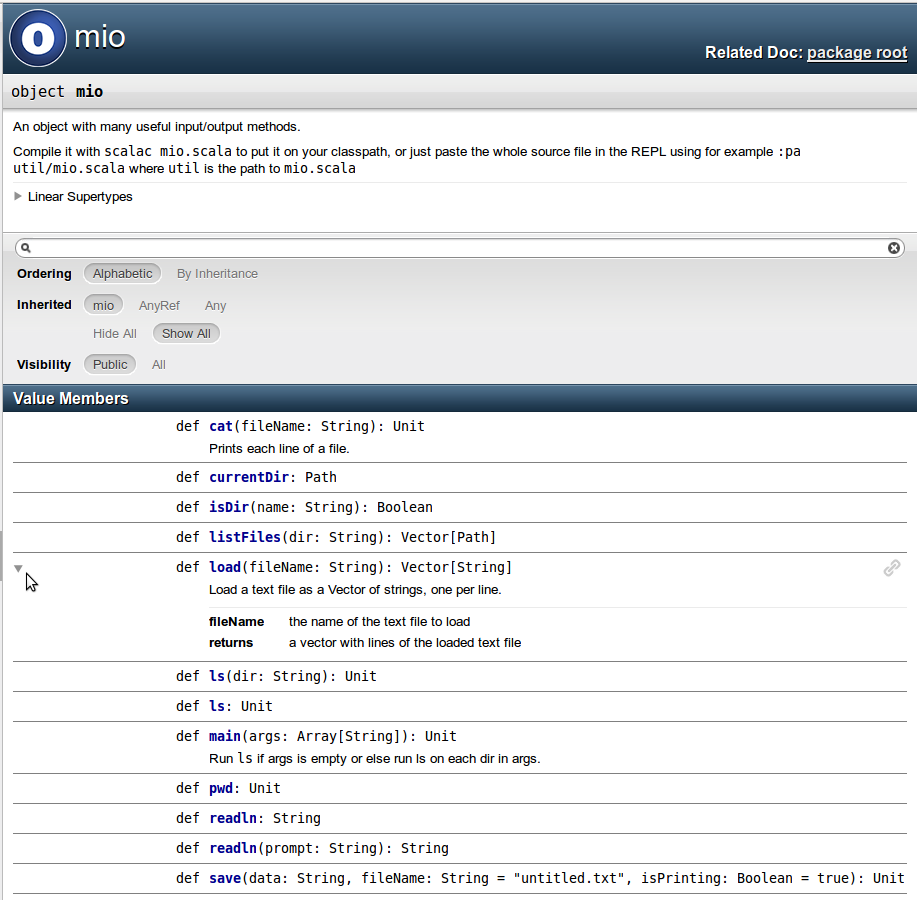
\includegraphics[width=1.0\textwidth]{../img/scaladoc/scaladoc-mio}
    \caption{Delar av en webbsida genererad med hjälp av \scaladoc. Mer detaljerade beskrivningar kan i förekommande fall vecklas ut eller in om man växlar mellan \Forward~och \MoveDown.}
    \label{fig:scaladoc:webpage}
\end{figure}


\subsection{Lära mer om scaladoc}

\begin{itemize}[leftmargin=*]

\item En video med tips om hur du söker och navigerar i \scaladoc-dokumentation: 
\\
\url{http://docs.scala-lang.org/overviews/scaladoc/interface.html}

\item
Riktlinjer för hur du skriver dokumentationskommentarer: \\
\url{http://docs.scala-lang.org/style/scaladoc.html}

\item Länksida till mer detaljerade beskrivningar: \\
\url{https://wiki.scala-lang.org/display/SW/Writing+Documentation} \\
inkluderande bland annat:

\begin{itemize}[nolistsep]
\item En beskrivning av syntaxen för formatering: \\
\url{https://wiki.scala-lang.org/display/SW/Syntax} 

\item En beskrivning av speciella annoteringar, t.ex. \code{@param}: \\
\url{https://wiki.scala-lang.org/display/SW/Tags+and+Annotations} 

\end{itemize}

\item Kör kommandot \texttt{ scaladoc -help } för att se användbara optioner.

\item \texttt{sbt doc} är ett smidigt sätt att generera api-dokumentation. Läs mer om \texttt{sbt} och api-dokumentation här: \\
\url{http://www.scala-sbt.org/0.13/docs/Howto-Scaladoc.html}


\end{itemize}

\clearpage

\section{javadoc}
\newcommand{\javadoc}{\texttt{javadoc}}


Med Java JDK följer dokumentationsverktyget \javadoc, som utifrån dokumentationskommentarer i Java-kod genererar en webbsajt med navigationslänkar. Webbsidor genererade med \javadoc~erbjuder inte samma funktioner för sökning och filtrering som \scaladoc, men det fungerar bra hitta det man söker om navigationslänkarna används tillsammans med webbläsarens inbyggda sökfunktion (Ctrlf+F).

\subsection{Använda dokumentation genererad med javadoc}

I figur \ref{fig:javadoc:overview} visas exempel på \javadoc~för biblioteket \code{cslib}. Om du klickar på ett paket kan du navigera till en översikt av innehållet i paketet. Om du klickar på en klass får du en översikt av klassens medlemmar, så som visas i \ref{fig:javadoc:class}.  Om du t.ex. klickar på ett metodnamn får du se mer detaljerade kommentarer. 

Ramarna till vänster på webbsidorna innehåller länkar till paket och klasser. Om du klickar på länken \textit{All Classes} överst till vänster för du en lista med navigationslänkar till alla tillgängliga klasser.De gulmarkerade rubrikerna visar vilken vy som är aktiv och navigationslänkar skrivs med blå text.

\begin{figure}
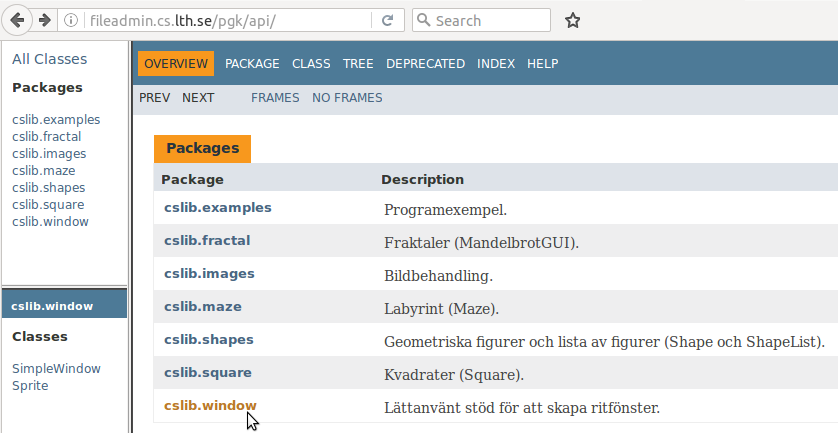
\includegraphics[width=1.0\textwidth]{../img/javadoc/javadoc-overview}
    \caption{Delar av en webbsida genererad med hjälp av \javadoc.}
    \label{fig:javadoc:overview}
\end{figure}



\begin{figure}
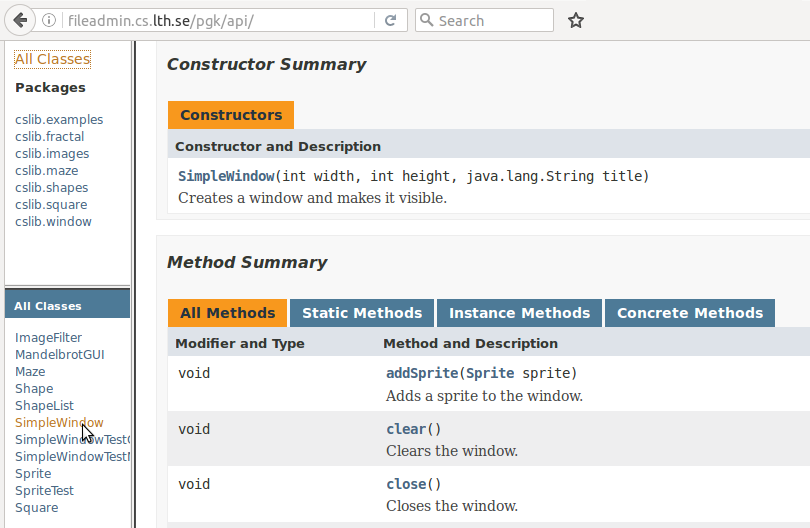
\includegraphics[width=1.0\textwidth]{../img/javadoc/javadoc-class}
    \caption{Delar av en webbsida med klassdokumentation genererad med hjälp av \javadoc.}
    \label{fig:javadoc:class}
\end{figure}






\subsection{Skriva dokumentationskommentarer för javadoc}

Kommentarer för \javadoc~och \scaladoc~ser ganska lika ut, även om det finns några skillnader. Det finns t.ex. inte lika många styrtecken för layouten i \javadoc~som i \scaladoc, och konventionen i Java är fyra blankstegs indrag och att fortsättningsrader i dokumentationskommentarer börjar asterisken under \textit{första} asterisken i öppningskommentaren. 

Nedan visas delar av \javadoc-kommentarerna för klassen \code{SimpleWindow} och dess konstruktor:
\begin{Code}[language=Java]
package cslib.window;
 
/** A simple window to draw in */
public class SimpleWindow {
   /**
    * Creates a window and makes it visible.
    * 
    * @param width   the width of the window
    * @param height  the height of the window
    * @param title   the title of the window
    */
    public SimpleWindow(int width, int height, String title) {
        ...
\end{Code}
Annoteringen \verb|@param| i början på en rad ger en speciell kommentar angående en parameter. Vid dokumentation av metoder kan annoteringen \verb|@return| användas i början av en rad för att skapa en speciell kommentar angående vad som returneras.

Övergripande dokumentation om innehållet i ett paket läggs i en textfil i paketets katalog med namnet \texttt{package-info.java}, se till exempel här: \\ {\href{https://github.com/lunduniversity/introprog/tree/master/workspace/cslib/src/main/java/cslib/window}{\small github.com/lunduniversity/introprog/tree/master/workspace/cslib/src/main/java/cslib/window}


Du kan läsa mer om hur man skriver \code{javadoc}-kommentarer här:\\
\href{http://www.oracle.com/technetwork/java/javase/documentation/index-137868.html}{www.oracle.com/technetwork/java/javase/documentation/index-137868.html}

% conversation of diffs between javadoc and scaladoc:
%  https://groups.google.com/forum/#!msg/scala-user/q-Vw03zcIVs/CaTR5XL-BQAJ

\subsection{Generera dokumentationskommentarer för javadoc}

Om du står i den katalog där din källkod finns, kan du med nedan kommando i terminalen gå igenom alla paket och underpaket och generera \javadoc-webbsidor i katalogen \texttt{doc}. Du kan därefter öppna dokumentationen i en webbläsare.
\begin{REPLnonum}[basicstyle=\color{white}\ttfamily\fontsize{9}{11}\selectfont]
$ javadoc -d doc -encoding UTF-8 -charset UTF-8 -sourcepath . -subpackages . *
$ firefox doc/index.html
\end{REPLnonum}
Ett smidigt sätt att generera både \scaladoc~och \javadoc~ är att använda \texttt{sbt}; det är bara att skriva \code{ sbt doc } i terminalen så genereras alla dokumentation för både Scala och Java i den katalog som \texttt{sbt} meddelar i sin resultatutskrift.

Om du lägger in nedan i \code{settings} i din \code{build.sbt} fungerar även svenska bokstäver och andra specialtecken på alla plattformar.
\begin{Code}
  javacOptions in (Compile, doc) ++= Seq(
    "-encoding", "UTF-8", 
    "-charset", "UTF-8", 
    "-docencoding", "UTF-8")
\end{Code}  

\noindent Du kan också använda din IDE för att köra \javadoc. I Eclipse, använd menyn \MenuArrow{Project}\Menu{Generate Javadoc...}, medan du i IntelliJ hittar motsvarande i menyn \MenuArrow{Tools}\Menu{Generate Javadoc...}
%!TEX encoding = UTF-8 Unicode
%!TEX root = ../compendium.tex

\newcommand{\sbt}{\texttt{sbt} }

\chapter{Byggverktyg}\label{appendix:build}

\section{Vad gör ett byggverktyg?}

Ett \textbf{byggverktyg} \Eng{build tool} används för att 
\begin{itemize}
\item ladda ner, 
\item kompilera, 
\item testköra, 
\item paketera och 
\item distribuera  
\end{itemize}
programvara. Ett stort utvecklingsprojekt kan innehålla många hundra kodfiler och under utvecklingens gång vill man kontinuerligt testköra systemet för att kontrollera att allt fortfarande fungerar; även den kod som inte ändrats, men som kanske ändå påverkas av ändringen. Ett byggverktyg används för att \textit{automatisera} denna process.

Ett viktigt begrepp i byggsammanhang är \textbf{beroende} \Eng{dependency}. Om koden X behöver annan kod Y för att fungera, sägs kod X ha ett beroende till kod Y. 

I konfigurationsfiler, som är skrivna i ett format som byggverktyget kan läsa, specificeras de beroenden som finns mellan olika koddelar. Byggverktyget analyserar dessa beroenden och, baserat på ändringstidsmarkeringar för kodfilerna, avgör byggverktyget vilken delmängd av kodfilerna som behöver \textbf{omkompileras} efter en ändring. Detta snabbar upp kompileringen avsevärt jämfört med en total omkompilering från grunden, som för ett stort projekt kan ta många minuter eller till och med timmar. Efter omkompilering av det som ändrats, kan byggverktyget instrueras att köra igenom testprogram och rapportera om testernas utfall, men även ladda upp körbara programpaket till t.ex. en webbserver.


En vanlig typ av beroende är färdiga programbibliotek som utnyttjas av systemet under utveckling, vilket i praktiken ofta innebär att en sökväg till en den kompilerade koden för programbiblioteket behöver göras tillgänglig. I JVM-sammanhang innebär detta att sökvägen till alla nödvändiga jar-filer behöver finnas på sökvägslistan kallad \textbf{classpath}. 

Många byggverktyg kan utföra så kallad \textbf{beroendeupplösning} \Eng{dependency resolution}, vilket innebär att nätverket av beroenden analyseras och rätt uppsättning programpaket görs tillgänglig under bygget. Detta kan även innebära att programpaket som är tillgängliga via nätet automatiskt laddas ned inför bygget, t.ex. via lagringsplatser för öppen källkod.   

Även om man bara har ett litet kodprojekt med några få kodfiler, är det ändå smidigt att använda ett byggverktyg. Man kan nämligen göra så att byggverktyget är aktivt i bakgrunden och, så fort man sparar en ändring av koden, gör omkompilering och rapporterar eventuella kompileringsfel.

Det är klokt att kompilera om ofta, helst vid varje liten ändring och rätta eventuella fel \textit{innan} nya ändringar görs, eftersom det är mycket lättare att klura ut ett enskilt problem efter en mindre ändring, än att åtgärda en massa svåra följdfel, som beror på en sekvens av omfattande ändringar, där misstaget begicks någon gång långt tidigare i ändringshistoriken. 

En integrerad utvecklingsmiljö, så som Eclipse+ScalaIDE eller IntelliJ IDEA, bygger om koden kontinuerligt och kan ofta kommunicera med flera olika typer av byggverktyg för att i samklang med dessa automatisera byggprocessen.

Det finns många olika byggverktyg. Några allmänt kända byggverktyg med öppen källkod listas nedan, tillsammans med namnen på deras konfigurationsfiler så att du ska känna igen vilket byggverktyg som används i  kodprojekt som du stöter på, t.ex. på GitHub.

\begin{itemize}
\item \sbt. Även kallad \textit{Scala Build Tool}. Användas för att bygga Java- och Scala-program i samexistens, men även för att automatisera en mängd andra saker. Byggverktyget är utvecklat i Scala och konfigurationsfilerna, som heter \texttt{build.sbt}, och innehåller Scala-kod som styr byggprocessen. 

\item \texttt{make}. Detta anrika byggverktyg har varit med ända sedan 1970-talet och används fortfarande för att bygga många Linux-system och är populärt vid utveckling med programspråken C och C++. Konfigurationsfilerna heter \texttt{Makefile} och har en egen, speciell syntax.

\item Apache \texttt{ant}. Detta byggverktyg är utvecklat i Java som ett alternativ till \texttt{make} och används fortfarande i många Java-projekt, även om Maven och Gradle (se nedan) är vanligare numera. Konfigurationsfilerna heter \texttt{build.xml} och skrivs i det standardiserade språket XML enligt  speciella regler.

\item Apache Maven, \texttt{mvn} är också skriven i Java och är en efterföljare till \texttt{ant}. Maven används av många Java-utvecklare. Konfigurationsfilerna heter \texttt{pom.xml} och innehåller en s.k. projektobjektmodell specificerad i XML enligt  speciella regler.

\item \texttt{gradle} bygger vidare på idéerna från \texttt{ant} och \texttt{maven} och är skrivet i Java och Groovy.  Konfigurationsfilerna skrivs i Groovy och heter \texttt{build.gradle}.  

\end{itemize} 

\section{Byggverktyget sbt}

Byggverktyget \sbt är skrivet i Scala och är det mest populära byggverktyget bland Scala-utvecklare. Med \sbt kan du skriva byggkonfigurationsfiler i Scala och även styra byggprocessen via ett interaktivt kommandoskal i terminalfönstret. Med inkrementell (stegvis) kompilering och parallellkörning av byggprocessens olika delar, kan den snabbas upp avsevärt.    


\subsection{Installera sbt}

\sbt finns förinstallerat på LTH:s datorer och körs igång med kommandot \sbt i terminalen.

Om du vill installera \sbt på din egen dator,
säkerställ först att du har \code{java} på din dator med terminalkommandot \code{java -version}. Om \code{java} saknas, följ instruktionerna i avsnitt \ref{appendix:compile:install-jdk} på sidan \pageref{appendix:compile:install-jdk}. 
Följ sedan instruktionerna här för att installera \sbt: \url{http://www.scala-sbt.org/download.html} 

\begin{itemize}

\item \textbf{Linux}. Om du surfar till ovan sida från en Linux-dator syns några terminalkommando som du använder för att installera \sbt i terminalen. 

\item \textbf{Windows}. Om du surfar till ovan sida från en Windows-dator visas en länk till en \code{.msi}-fil. Ladda ner och dubbelklicka på den.

\item \textbf{macOS}. Följ instruktionerna under rubriken \textit{Manual Installation}.

\end{itemize}

\noindent När du kör sbt första gången kommer ytterligare filer att laddas ner och installeras och delar av denna process kan ta lång tid. Ha tålamod och avbryt inte körningen, även om inget speciellt ser ut att hända på ett bra tag.

\subsection{Anpassa sbt}
För att följa de versioner av \sbt och Scala som vi använder i kursen, skapa med hjälp av editor en textfil med namnet \code{global.sbt} i katalogen \code{.sbt} som ligger i din hemkatalog efter att du installerat klart \sbt. Fråga vid behov någon om hjälp om hur man hittar dolda filer i ditt operativsystem, då filer som börjar med punkt ibland inte syns i filbläddraren. Filen ska ha följande innehåll:
\begin{Code}
scalaVersion := "2.11.8"

sbtVersion := "0.13.12"
\end{Code} 

\noindent När du kör igång \sbt igen kommer ovan inställningar eventuellt medföra vissa nedladdningar, men när det är gjort har du rätt versioner tillgängliga och \sbt kommer att starta snabbt nästa gång.


\subsection{Använda sbt}
\sbt är konstruerat för att klara mycket stora projekt, men det är enkelt att använda \sbt också om du bara har ett litet projekt med någon enstaka kodfil. Med \sbt installerat, är det bara att skriva 
\begin{REPLnonum}
$ sbt run
\end{REPLnonum} 
i terminalen i det bibliotek där dina kodfiler ligger. \sbt letar då upp och kompilerar alla de \code{.scala}-filer som ligger i biblioteket och, om det bara finns ett objekt med main-metod, kör \sbt igång denna main-metod direkt, förutsatt att kompileringen kan avlutas utan fel. Även \code{.java}-filer kompileras automatiskt om de ligger i samma bibliotek.

Om du enbart skriver \sbt körs det interaktiva kommandoskalet igång, där du kan köra kommando så som \code{compile} och \code{run}. Om du skriver ett \code{~} före kommandot \code{run}, enligt nedan kommer \sbt vara aktivt i bakgrunden medan du editerar och så fort du sparar en ändring kommer omkompilering av ändrade kodfiler ske, varefter main-metoden exekveras om kompileringen lyckades. 
 
\begin{REPLnonum}
$ sbt
[info] Set current project to bjornr (in build file:/home/bjornr/)
> ~run
[info] Compiling 1 Scala source to /home/bjornr/target/scala-2.11/classes...
[info] Running hello 
Hello, World!
[success] Total time: 1 s, completed Aug 4, 2016 10:05:17 PM
1. Waiting for source changes... (press enter to interrupt)
[info] Compiling 1 Scala source to /home/bjornr/target/scala-2.11/classes...
[info] Running hello 
Hello again, World!
[success] Total time: 0 s, completed Aug 4, 2016 10:05:25 PM
2. Waiting for source changes... (press enter to interrupt)

\end{REPLnonum} 

\noindent I ovan körning gör sbt en omkompilering, efter att en ändring av utskriftssträngen sparats.

\begin{Code}
// in file hello.scala

object hello {
  def main(args: Array[String]): Unit = {
    println("Hello again, World!") // added 'again' then Ctrl+S 
  }
}
\end{Code}


\subsubsection{Katalogstruktur}

Om man har kod i underkataloger förutsätter \sbt att du följer en viss, specifik katalogstruktur. Denna katalogstruktur används även av andra byggverktyg, så som Maven, och fungerar även i många utvecklingsmiljöer så som Eclipse och IntelliJ. 

Det blir också mindre rörigt och lättare för alla att hitta i projektets kataloger om dina kodfiler placeras i en given struktur som är allmänt accepterad.
Placera därför gärna dina kodfiler i underkataloger enligt strukturen som visas i figur \ref{fig:sbt:dir-structure}. 

\begin{figure}[H]
\centering

\begin{lstlisting}[frame=none, backgroundcolor=]
					src/
					  main/
					    resources/
					       <files to include in main jar here>
					    scala/
					       <main Scala sources>
					    java/
					       <main Java sources>
					  test/
					    resources
					       <files to include in test jar here>
					    scala/
					       <test Scala sources>
					    java/
					       <test Java sources>
\end{lstlisting}

\caption{Katalogstrukturen i ett \sbt-projekt. Bara de kataloger som har något innehåll behöver finnas.}
\label{fig:sbt:dir-structure}
\end{figure}

\noindent Lägg enligt denna struktur dina \code{.scala}-filer i underkatalogen \code{src/main/scala/} och dina \code{.java}-filer i underkatalogen \code{src/main/java/}. Om du lägger kod i biblioteken  \code{src/test/scala/} respektive \code{src/test/java/} kommer denna kod köras när du skriver \sbt-kommandot \code{test}. Om du lägger filer i underkatalogen \code{src/main/resources/} kommer dessa att paketeras med i jar-filen som skapas när du kör \sbt-kommandot \texttt{package}.

Om du använder t.ex. \code{package x.y.z;} i din Java-kod, måste även strukturer på underkataloger matcha och kodfilen alltså ligga i  \code{src/main/java/x/y/z/}.

I Scala är det egentligen inte nödvändigt att koden ligger i samma bibliotek som de kompilerade \texttt{.class}-filerna, men det kan vara bra att följa paketstrukturen även för Scala-källkoden; speciellt om du senare vill kunna köra din kod med Eclipse, som kräver denna överensstämmelse mellan paket och källkodskataloger, inte bara för Java, utan även för Scala.


\subsubsection{Konfigurera dina byggen i filen \code{build.sbt}}

Om du vill göra inställningar och även hjälpa andra att kunna återskapa dina byggen, så skapa en konfigurationsfil med namnet \code{build.sbt} och placera den i projektets baskatalog. Figur \ref{fig:sbt:build-file} visar en enkel byggkonfigurationsfil. Där väljer du namn på ditt projekt, sätter ett versionsnummer på ditt bygge, samt specificerar vilken version av Scala-kompilatorn du använder. Det senare är viktigt för att andra ska kunna bygga din kod under samma förutsättningar som du. 

\begin{figure}[H]
\centering
\begin{Code}
lazy val root = (project in file(".")).
  settings(
    name := "hello",
    version := "1.0",
    scalaVersion := "2.11.8"
  )
\end{Code}
\caption{En enkel konfigurationsfil för \sbt som innehåller det som kallas en \textit{build definition} i \texttt{sbt}-termer. Filen ska ha namnet \code{build.sbt} och vara placerad i projektets baskatalog.}
\label{fig:sbt:build-file}
\end{figure}

\noindent Du kan läsa mer om alla möjligheter med \sbt och hur man skapar mer avancerade byggkonfigurationsfiler här: \\
\url{http://www.scala-sbt.org/0.13/docs/}

Du hittar ett exempel på en avancerad byggdefinition i kursens repo, som har många aggregerade underprojekt, bl.a. för att bygga detta kompedium med \code{pdflatex}. I byggdefinitionen instrueras även \sbt att bygga kursens workspace, samt att generera de speciell projektfiler som Eclipse+ScalaIDE kräver med en \sbt-plugin. Filen finns här: \\
\url{https://github.com/lunduniversity/introprog/blob/master/build.sbt}

\subsubsection{Lägga till beroenden}

\TODO 

\url{http://search.maven.org}


%!TEX encoding = UTF-8 Unicode
%!TEX root = ../compendium.tex


\chapter{Versionshantering och kodlagring}

\section{Vad är versionshantering?}

\textbf{Versionshantering}\footnote{\href{https://en.wikipedia.org/wiki/Version_control}{en.wikipedia.org/wiki/Version\_control}} \Eng{version control eller revision control} av mjukvara innebär att hålla koll på olika versioner av koden i ett utvecklingsprojekt allteftersom koden ändras. Versionshantering är en deldisciplin inom \textbf{konfigurationshantering} \Eng{software configuration managament} som inbegriper allt i processen för att identifiera, besluta, genomföra och följa upp ändringar.

En viktig del av versionshantering är att \textit{lagra} olika versioner av koden allt eftersom den utvecklas, så att tidigare versioner kan \textit{återskapas} vid behov. Ett bra verktygsstöd och en väldefinierad arbetsprocess för versionshanteringen, som alla i utvecklingsprojektet följer, möjliggör att flera utvecklare kan \textit{arbeta parallellt} med att sammanfoga \Eng{merge} varandras tillägg och ändringar i den gemensamma kodbasen utan att det blir kaos och förvirring.

God versionshantering är helt avgörande för utvecklarnas produktivitet, speciellt för stora projekt med många utvecklare som jobbar parallellt mot en omfattande kodbas med många olika interna och externa komponenter. 
Men även ett litet projekt med en enda utvecklare kan ha god nytta av ett versionshanteringsverktyg och ett disciplinerat förfarande för att namge versioner, t.ex. för att kunna återskapa tidigare versioner av projektets olika kodfiler när en ändring visar sig mindre lyckad.   

Det finns flera olika modeller för hur kodlagringen sker:
\begin{itemize}
\item \textbf{lokal}; alla utvecklare jobbar i samma, lokala filsystem där alla olika versioner lagras.
\item \textbf{centraliserad}; ett repositorium (förk. repo), alltså en databas med koden, finns centralt på en server som alla jobbar mot med hjällp av en versionshanteringsklient.
\item \textbf{distribuerad}; alla utvecklare har sitt eget lokala repo och varje utvecklare initierar enskilt delning av ändringar mellan olika repo. 
\end{itemize}


\section{Versionshanteringsverktyget Git}

Det finns många olika versionshanteringsverktyg\footnote{\href{https://en.wikipedia.org/wiki/List_of_version_control_software}{https://en.wikipedia.org/wiki/List\_of\_version\_control\_software}}
 som använder olika modeller för kodlagring; lokal, centraliserad, distribuerad eller kombinationer därav. 
På senare tid har verktyget \textbf{Git}\footnote{\href{https://en.wikipedia.org/wiki/Git_(software)}{https://en.wikipedia.org/wiki/Git\_(software)}} fått en stark ställning, speciellt i öppenkällkodsvärlden. Git utvecklades ursprungligen av Linus Torvalds för att versionshantera Linuxkärnan, men har växt till ett omfattande öppenkällkodsprojekt med stor spridning och många användare och bidragsgivare. 

Git är skapad för \textbf{distribuerad} versionshantering där var och en kan jobba snabbt och smidigt i sitt eget lokala repo, utan att behöva vänta på att en klient ska synkronisera koden med ett centralt repo på en server över nätverket. Ändringar delas mellan repo på begäran ev enskilda utvecklare. 

Varje ny version av koden lagras som en avgränsad mängd ändringar sedan förra versionen, en s.k. \textbf{commit}%
\footnote{På svenska kan t.ex. ''inlämning'' användas, men låneordet commit är redan etablerat.}%
, och hanteras internt av Git i en lokal databas i katalogen \code{.git} som ligger överst i din projektkatalog. Genom olika kommandon i terminalen, eller via en klient med ett grafiskt användargränssnitt, kan din kod överföras till och från den lokala koddatabasen, alternativt delas med andra repon via nätet. 

Det finns en välskriven bok kallad \textit{''Pro Git''} som förklarar Git på djupet och är tillgänglig fritt här: 
\url{https://git-scm.com/book/en/v2}.
Läs kapitel 1 och 2 så får du en bra grund att stå på. 

Dessa termer är bra att kunna utantill innan du kör igång med Git:
\newcommand{\TermItem}[3]{\item \textbf{#1} (\textit{substantiv}: #2, \textit{verb}: #3).}
\begin{itemize}

\item \textbf{repo} (\textit{substantiv}: ett repositorium, \textit{eng. a repository}) En koddatabas med ändringshistorik. 

\TermItem{commit}{en inlämning}{att lämna in} 
  En avgränsad mängd nya ändringar lämnas in i det lokala repot. Repots ändringshistorik utgörs av sekvensen av alla inlämningar.

\TermItem{push}{en leverans}{att leverera, att trycka upp} En eller flera inlämningar trycks upp till ett annat repo.

\TermItem{pull}{en hämtning}{att hämta, att dra ner} En eller flera inlämningar dras ner från ett annat repo.

\TermItem{merge}{en ihopslagning}{att sammanfoga} En eller flera inlämningar slås samman till en ny inlämning. 

\item \textbf{merge conflict} (\textit{substantiv}: en sammanfogningskonflikt, \textit{eng. a merge conflict}) Problem vid sammanfogning; ändringar kan inte enkelt sammanfogas på ett entydigt sätt.

\item \textbf{pull request} (förk. PR, \textit{substantiv}: en hämtningsbegäran, \textit{verb}: att begära en hämtning). Utvecklare A ber en annan utvecklare B att hämta en eller flera inlämningar från A:s repo och sammanfoga med B:s repo.

\end{itemize}

\subsection{Installera git}\label{subsection:install-git}

Git finns förinstallerat på LTH:s Linuxdatorer. Du kan kolla om Git redan finns på din maskin genom att skriva \code{git help} i terminalen. 

Det finns bra instruktioner om hur du installerar Git på din egen maskin här: \url{https://git-scm.com/book/en/v2/Getting-Started-Installing-Git}

Om du vill ha en Git-klient med grafiskt användargränssnitt finns det många att välja på, se här:  \url{https://git-scm.com/downloads/guis} 

Om du inte vet vilken du ska välja, prova GitKraken som är gratis (men stängd) och finns för alla plattformar: \url{https://www.gitkraken.com/}.


\subsection{Anpassa Git}

Innan du börjar använda git, konfigurera ditt användarnamn och din email med nedan terminalkommando, där du anger ditt användarnamn i stället för \code{fornamnefternamn} och din mejladress i stället för \code{mejladr@plats.se}:
\begin{REPLnonum}
$ git config --global user.name fornamnefternamn
$ git config --global user.email mejladr@plats.se
\end{REPLnonum}
Det är bra att välja \textit{ett} användarnamn, för \textit{alla} repo, även kodlagringsplatser på nätet; förslagsvis \code{fornamnefternamn} utan svenska tecken,  så att du blir lätt att känna igen, speciellt om du jobbar med öppen källkod där ditt namn kommer associerat med alla de kodbidrag du gör under ditt yrkesliv.

Läs mer om hur du gör andra inställningar här, t.ex. hur du anger vilken editor som git startar när du ska skriva commit-beskrivningar: \\ \url{https://git-scm.com/book/en/v2/Getting-Started-First-Time-Git-Setup}
  
  
\subsection{Använda git}

Nedan listas några vanliga terminalkommandon i Git.

\begin{itemize}[leftmargin=*]

\item Skapa ett repo i en katalog:
\begin{REPLnonum}
$ cd myproject
$ git init
\end{REPLnonum} 

\item Se vilka filer som ändrats och ännu ej lämnats in:
\begin{REPLnonum}
$ git status
$ git status -s
\end{REPLnonum} 

\item Se vilka ändringar som gjorts i filer som ännu ej lämnats in:
\begin{REPLnonum}
$ git diff 
\end{REPLnonum} 

\item Se vilka inlämningar som finns i ändringshistoriken:
\begin{REPLnonum}
$ git log 
$ git log --oneline -5
\end{REPLnonum} 

\item Lägg till filer som ska ingå i nästa inlämning och gör sedan inlämningen; ge inlämningen en bra beskrivning som förklarar vad inlämningen omfattar:
\begin{REPLnonum}
$ git add *.scala
$ git commit -m 'initial project version'
\end{REPLnonum} 

\item Ångra alla tillägg inför inlämning (ändringarna finns kvar och kan läggas till igen om du vill):
\begin{REPLnonum}
$ git reset 
\end{REPLnonum} 

\item Skippa de senaste, ännu ej commitade, ändringar i filen \code{filename}, ''\textit{undo}''. Används om du är helt säker på att du vill ångra dina senaste ändringar.
\\ \mbox{\colorbox{red!30}{VARNING!} Dina senaste ändringar i filen förloras för alltid; kan ej ångras!}   
\begin{REPLnonum}
$ git checkout filename 
\end{REPLnonum} 

\item Man vill förhindra versionshantering av vissa filer, t.ex. binärkodsfiler så som \code{.class}-filer och andra genererade filer. Detta gör du genom att skapa en fil med namnet \code{.gitignore} och lägga in filändelser enligt nedan syntax, där \code{**/} avser alla kataloger och underkataloger och \code{*} kan vara vilken början på ett filnamn som helst. Symbolen \code{#} föregår en kommentarsrad.
\begin{Code}[language=]
# this is my .gitignore

# Latex
**/*.aux
**/*.log
**/*.nav
**/*.out
**/*.snm
**/*.vrb
**/*.synctex.gz
**/*.synctex.gz(busy)
**/*.toc

# Java / Scala
**/*.class

# Sbt
**/target

\end{Code} 


\end{itemize}
 

\clearpage 
  
\section{Kodlagringsplatser på nätet}\label{section:code-hosting}

Många utvecklare använder kodlagringsplatser på nätet (''i molnet''). \Eng{code hosting} för att underlätta samarbete kring kod och för att dela med sig av öppen källkod. Det finns många olika kodlagringsplatser som kan användas gratis under vissa förutsättningar eller mot betalning med tillhörande extratjänster. 

Nedan beskrivs några vanliga nätplatser för öppen och sluten kodlagring, som alla är Git-baserade:

\begin{itemize}
\item  \textbf{GitHub}, \url{https://github.com}, är en av de mest populära kodlagringsplatserna för öppen källkod, men har även blivit en populär plats för jobbsökande utvecklare att visa upp sina  kodarbetsprover för framtida arbetsgivare. GitHub är gratis att använda för dig som privatperson om du låter ditt repo vara öppet att läsa för alla. Det kostar pengar om du vill ha ett slutet repo. Många företag betalar GitHub för att lagra sin stängda kod med tilläggstjänster för att testa, bygga och driftsätta kod etc. Koden som styr själva kodlagringsplatsen GitHub är stängd, till skillnad från GitLab.

\item \textbf{BitBucket}, \url{https://bitbucket.org}, är en populära kodlagringsplats både för öppen och stängd källkod och drivs av det australiensiska företaget Atlassian. Det är gratis för privatpersoner och små team att ha både öppna och slutna repon, men bara om det är få bidragsgivare. Kostnader tillkommer om antalet bidragsgivare kommer över en viss nivå. Universitetsanställda och studenter kan få mer gynnsamma villkor efter ansökan. Atlassian erbjuder en hel verktygssvit för att hantera buggar och samarbeta över nätet. BitBucket stödjer, förutom Git, även andra versionshanteringsverktyg.

\item \textbf{GitLab}, \url{https://gitlab.com}, erbjuder gratis kodlagring för öppen källkod, men det är även gratis för privatpersoner och gemenskapsprojekt att ha stängda repo. Företag kan betala för stängd kodlagring med extratjänster för att testa, bygga och driftsätta kod etc. GitLab är i sig ett öppenkällkodsprojekt och koden som styr kodlagringsplatsen är öppen och fri. Detta innebär att du själv kan ladda ner koden och starta en kodlagringsplats. LTH har en GitLab-baserad kodlagringsplats här: \url{https://git.cs.lth.se}

\end{itemize}

\subsubsection{Använda kodlagringsplatser}

Det är bra att registrera ditt användarnamn, förslagsvis \code{fornamnefternamn} som ett ord utan svenska tecken, på någon eller alla av ovan sajter, dels för att paxa ditt namn och dels för börja samarbeta med utvecklarvänner världen över. Om du inte vet vilken du ska välja, börja med \url{https://github.com}. Om du vill ha både öppna och slutna repon gratis, testa \url{https://gitlab.com}. 

Med en Git-baserad kodlagringsplats för du möjlighet att synka ditt lokala repo mot en server på nätet med hjälp av \code{git}-kommandon i terminalen eller via en Git-klient med grafiskt användargränssnitt, se avsnitt \ref{subsection:install-git}. 

Innan du börjar använda en kodlagringsplats är det bra att sätta sig in i begreppen nedan.

\begin{itemize}
\TermItem{clone}{en klon är kopia av ett (nätlagrat) repo}{att klona, att skapa en kopia} Genom att klona ett repo som ligger på en nätlagringsplats kan du bygga, undersöka och vidareutveckla koden lokalt på din dator. Om du har rättigheter att lämna in kod till det centrala orginalet kan du pusha dina commits direkt via terminalkommando eller Git-klient.

\TermItem{fork}{en förgrening av ett helt repo}{att förgrena ett repo, att ''forka''} Genom att förgrena ett repo skapar du en kopia, normalt även den nätlagrad på en kodlagringsplats, som du kan utveckla separat från orginalet. Det blir då möjligt för dig att lämna in ändringar och trycka upp dem, även om du inte har rättigheter att leverera (''pusha'') till originalet. Gör en ändringsbegäran (Pull Request, PR) om du vill bidra med dina ändringar, så kan ägaren av orginalet sedan välja att sammanfoga (''merga'') dina ändringar med orginalet. Många nätlagringsplatser, så som GitHub, har en speciell knapp som du trycker på för att enkelt skapa en fork av ett repo under din användare. 

\item \textbf{upstream} (\textit{preposition}: uppströms, \textit{substantiv}: uppströmsrepo) Ett uppströmsrepo utgör orginal till ett förgrenat repo (en ''fork''). 
\begin{itemize}[noitemsep,nolistsep]

\item Här beskrivs hur du länkar en förgrening uppströms: \\ 
{\small\url{https://help.github.com/articles/configuring-a-remote-for-a-fork/}}

\item Här beskrivs hur du synkar en förgrening uppströms:\\
{\small\url{https://help.github.com/articles/syncing-a-fork/}}

\end{itemize}

\end{itemize}

Om du vill bidra till ett öppenkällkodsprojekt, börja med att forka repot på kodlagringsplatsen och sedan klona repot till din lokala dator. Därefter kan du commita ändringar och pusha till din fork och slutligen gör en pull request från din fork till upstream. Läs om hur ett bidrag kan gå till i avsnitt \ref{section:OSS-contribution-example}.

Här följer några användbara kommandon:

\begin{itemize}
\item Skapa en lokal kopia av ett fjärran \Eng{remote} repo; här visas hur du klonar kursens repo från GitHub:
\begin{REPLnonum}
$ git clone --depth 1 https://github.com/lunduniversity/introprog
\end{REPLnonum} 

\item Dra ner nya inlämningar från ett fjärran repo:
\begin{REPLnonum}
$ git pull 
\end{REPLnonum} 

\item Trycka upp nya lokala inlämning till ett fjärran repo:
\begin{REPLnonum}
$ git push 
\end{REPLnonum} 

\end{itemize}



%!TEX encoding = UTF-8 Unicode
%!TEX root = ../compendium.tex

\chapter{Virtuell maskin}\label{appendix:vbox}

\section{Vad är en virtuell maskin?}

Du kan köra alla kursens verktyg i en så kallad \textbf{virtuell maskin} (förk. vm, eng. \textit{virtual machine}). 
Detta är ett enkelt och säkert sätt köra ett annat operativsystem i en ''sandlåda'' som inte påverkar din dators ursprungliga operativsystem. Figur \ref{fig:vm} visar kursens virtuella maskin med sin exklusiva bakgrundsbild. Exekveringen av en vm sker på en \textbf{värddator} \Eng{host}. I figur \ref{fig:vm} körs kursens vm i en Linux-värd med virtualiseringsapplikationen \textit{VirtualBox}\footnote{\href{https://en.wikipedia.org/wiki/VirtualBox}{/en.wikipedia.org/wiki/VirtualBox}}, som är öppen och gratis och även finns för Windows- och macOS-värdar. 



\begin{figure}[H]
\centering
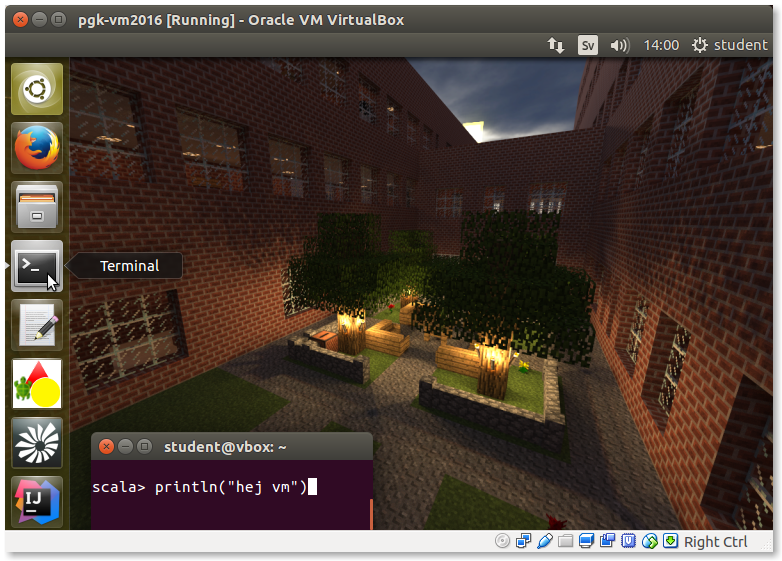
\includegraphics[width=1.0\textwidth]{../img/vm.png}
\caption{Den virtuella maskinen pgk-vm2016.}
\label{fig:vm}
\end{figure}


\section{Vad innehåller kursens vm?}

Kursens virtuell maskin har alla verktyg som du behöver förinstallerade.  Vår vm kör Ubuntu 16.04.1 med fönstermiljön Unity, vilket är samma miljö som körs på Linuxdatorerna i E-huset på LTH. 

Detta och mycket annat är förinstallerat i kursens vm:

\begin{itemize}
\item \texttt{java} och \texttt{javac} med JDK 8
\item \texttt{scala} och \texttt{scalac} med Scala 2.11.8
\item Kojo 2.4.09
\item Eclipse Mars.2 med ScalaIDE 4.4.1
\item InteliJ IDEA 2016.2 med Scala-plugin
\item \texttt{gedit}
\item \texttt{git}
\item \texttt{sbt}
\item \texttt{pdflatex} (inkl. texlive-full, texlive-lang-europe, texworks, m.m.) 
\item \texttt{amm} 0.7.0, för Scala-skriptning, se \url{http://www.lihaoyi.com/Ammonite/}
\item Alla skrivbordsappar som kommer med Unbuntu, t.ex. LibreOffice för ordbehandling och kalkylblad  kompatibel med MS Word och MS Excel.  
\item Kursens repo i katalogen \code{~/git/lunduniversity/introprog/} inklusive  \texttt{compendium/compenium.pdf} och kursens \texttt{workspace}.
\item Den maximalt avskalade fönstermiljön \url{https://i3wm.org/} om du gillar att jobba effektivt med tangentbordskortkommandon. Logga först ut genom att klicka i systemmenyn längst uppe till höger och välj sedan i3 i rullgardingsmenyn som trillar ner när du klickar på Ubuntu-symbolen ovanför lösenordsrutan på inloggningsskärmen.
\end{itemize}

\section{Installera kursens vm}

Det går lite långsammare att köra i en virtuell maskin jämfört med att köra direkt ''på metallen'', då det sker vissa översättningar och kontroller under virtualiseringsprocessen som annars är onödiga. Och den virtuella maskinen behöver få en rejäl andel av din dators minne. Så för att köra en virtuell maskin utan att det ska bli segt behövs en ganska snabb processor, gärna över 2.5 GHz, och ganska mycket minne, gärna mer än 4GB. 

Även om det går lite segt är en virtuell maskin ett utmärkt sätt att prova på Linux och Ubuntu. Eftersom man lätt kan spara undan en hel maskin är det ett bra sätt att experimentera med olika inställningar och installationer utan att ens normala miljö påverkas. Och kör du terminalfönster och en enkel editor brukar svag prestanda och lite minne inte vara ett stort problem.\footnote{Om du tycker det går alltför segt kan du istället installera Linux direkt på din dator jämsides ditt andra operativsystem -- fråga någon som vet om hur man gör detta.} 

Gör så här för att installera VirtualBox och köra kursens virtuella maskin:
\begin{enumerate}
\item  Ladda ner VirtualBox v5 för ditt operativsystem här och installera: \\ \url{https://www.virtualbox.org/wiki/Downloads}

\item Ladda även ner \textit{''VirtualBox Oracle VM VirtualBox Extension Pack''}  och installera enligt instruktionerna här:\\ \url{https://www.virtualbox.org/wiki/Downloads} \\ Om du stöter på problem eller undrar hur, fråga någon om hjälp.

\item Det kan hända att du får felmeddelande som innehåller något som liknar ''Intel VT-x'' eller ''Hyper-V'', så som beskrivs här:
\\ \href{http://www.howtogeek.com/213795/how-to-enable-intel-vt-x-in-your-computers-bios-or-uefi-firmware/}{www.howtogeek.com/213795/how-to-enable-intel-vt-x-in-your-computers-bios-or-uefi-firmware}\\
Då behöver du tillåta virtualiseringsfunktioner i BIOS på din dator. Om du inte vet hur du ska göra detta, be någon som vet om hjälp.

\item     Ladda ner filen \texttt{pgk-vm2016.ova} här: \\ \url{http://fileadmin.cs.lth.se/pgk/pgk2016.ova} \\ OBS! Då filen är på nästan 10GB kan nedladdningen ta \textit{mycket} lång tid, kanske flera timmar beroende på din internetuppkoppling. Har du problem med nedladdningstider kan du prova att ladda ner filen till ett USB-minne på skolans datorer, så att nedladdningen sker lokalt i E-huset.

\item     Öppna VirtualBox och välj \MenuArrow{File}\Menu{Import appliance..} och bläddra till filen \code{pgk-vm2016.ova} och klicka \Button{Next} och sedan \Button{Import}. Själva importen kan ta lång tid, kanske flera tiotals minuter beroende på hur snabbt din dator läser från disk.

\item Markera maskinen \textbf{pgk-vm2016} och välj menyn \MenuArrow{Machine}\Menu{Settings...} (eller tryck Ctrl+S) och undersök inställningarna. Se speciellt under fliken \textbf{System} och \textbf{Motherboard} där det står hur mycket \textbf{Base memory} du tilldelar. Om du har gott om minne kan du med fördel öka minnet till 4096MB, speciellt om du tänker köra igång de tungkörda IDE-apparna Eclipse eller IntelliJ.

\item Starta maskinen \textbf{pgk-vm2016} med ett dubbelklick. Ha lite tålamod innan maskinen är igång. Du kan behöva justera skärmstorleken i värdmaskinsmenyn \Menu{View}.

\item Öppna ett terminalfönster och skriv \texttt{scala} och du är igång och kan börja göra övningarna i detta kompendium!

\item Du behöver inte logga in för att köra igång maskinen under användaren \code{student}, men du  behöver lösenordet\footnote{\code{pgkBytMig2016}} för att installera nya program.

\item Börja med att uppdatera mjukvaran på din virtuella maskin genom att köra dessa terminalkommando:
\begin{REPLnonum}
$ sudo apt-get update
$ sudo apt-get upgrade
$ sudo apt-get dist-upgrade
\end{REPLnonum}


\item För att dra ner de senaste inlämningarna i kursrepot och uppdatera kompendiet och workspace, kör följande terminalkommando:
\begin{REPLnonum}
$ cd ~/git/lunduniversity/introprog
$ git pull
$ sbt build
$ sbt eclipse
\end{REPLnonum}

\item Om allt verkar fungera fint kan du nu prova att sätta på 3D-accelereringen för snabbare grafikrendering. Stäng maskinen genom att välja \Menu{Shut Down...} i systemmenyn. Ändra inställningar i menyn \MenuArrow{Settings...}\Menu{Display} genom att i fliken \textbf{Acceleration} under \textbf{Screen} markera \FramedCheckmark{Enable 3D acceleration}. Stara maskinen. Om det fungerar så blir animeringar avsevärt snyggare och smidigare. Om det inte fungerar, stäng av maskinen med \Menu{Power off} och avmarkera \FramedUnchecked{Enable 3D acceleration} igen.\footnote{Du kan också prova att genomföra stegen som visas här, för att ominstallera vissa saker som kan ha uppdaterats sedan detta skrevs: \url{https://www.linuxbabe.com/virtualbox/how-to-install-virtualbox-guest-additions-on-ubuntu-step-by-step}}

\end{enumerate}
%!TEX encoding = UTF-8 Unicode
%!TEX root = ../compendium.tex

\chapter{Hur bidra till kursmaterialet?}\label{appendix:contrib}

\section{Bidrag är varmt välkomna!}

Ett av huvudsyftena med att göra detta kursmaterial fritt och öppet är att möjliggöra bidrag från alla som är intresserade. Speciellt välkommet är bidrag från studenter som vill vara delaktiga i att utveckla undervisningen.

\section{Instruktioner}

\subsection{Vad behövs för att kunna bidra?}

Om du hittar ett problem, t.ex. ett enkelt stavfel, eller har något mer omfattande som borde förbättras, men ännu inte känner till eller har tillgång till de verktyg som beskriv nedan och som behövs för att göra bidrag, kontakta då någon som redan bidragit till materialet, så att någon annan kan implementera ditt förslag.

Innan du själv kan implementera ändringar direkt i materialet, behöver du känna till, och ha tillgång  till, ett eller flera av följande verktyg (beroende på vad ändringen gäller):

\begin{itemize}[noitemsep]
\item Latex: \href{https://en.wikibooks.org/wiki/LaTeX}{en.wikibooks.org/wiki/LaTeX}
\item Scala: \href{https://en.wikipedia.org/wiki/Scala\_\%28programming_language\%29}{en.wikipedia.org/wiki/Scala\_\%28programming\_language\%29}
\item git: \href{https://en.wikipedia.org/wiki/Git\_\%28software\%29}{https://en.wikipedia.org/wiki/Git\_\%28software\%29}
\item GitHub: \href{https://en.wikipedia.org/wiki/Github}{en.wikipedia.org/wiki/Github}
\item sbt: \href{https://en.wikipedia.org/wiki/SBT\_\%28software\%29}{en.wikipedia.org/wiki/SBT\_\%28software\%29}
\end{itemize}
Läs mer om hur du bidrar här: \\ \href{https://github.com/lunduniversity/introprog#how-to-contribute-to-this-repo}{github.com/lunduniversity/introprog\#how-to-contribute-to-this-repo}



\subsection{Svenska eller engelska?}

Vi blandar engelska och svenska enligt följande principer:

\begin{itemize}

\item Publika diskussioner, t.ex. i issues och pull requests på GitHub, sker på engelska. I en  framtid kan delar av materialet komma att översättas till engelska och då är det bra om även icke-engelskspråkiga kan förstå vad som har hänt. Alla ändringshändelser sparas och man kan söka och gå tillbaka i historiken.

\item Kompendiet finns för närvarande bara på svenska eftersom kursen initialt endast ges för svenskspråkiga studenter, men texten ska hjälpa läsaren att tillgodogöra sig motsvarande engelsk terminologi. Skriv därför mostvarande engelska begrepp \Eng{concept} i parentes med hjälp av latex-kommandot \verb+\Eng{concept}+.

\item På övningar och föreläsningar är svenska variabelnamn ok. Svenska kan användas för att hjälpa den som håller på att lära sig att skilja på ord som vi själv hittar på och ord som finns i programmeringsspråket. Detta signalerar också att när man lär sig och experimenterar kan man hitta på tokroliga namn och använda svenska hur mycket man vill. Man lär sig genom att prova!

\item Kod i labbar ska vara på engelska. Detta signalerar att när man kodar för att det ska bli något bestående, då kodar man på engelska.

\end{itemize}

\section{Exempel}\label{section:OSS-contribution-example}

Som exempel på hur det går till i ett typiskt öppen-källkodsprojekt, beskrivs nedan vad som hände i ett verkligt fall: en dokumentationsuppdatering av Scala-dokumentationen efter att ett fel upptäckts. Detta exempelfall är ett typiskt scenario som illustrerar hur det kan gå till, och vad man kan behöva tänka på. Exemplet ger också länkar till och inblick i ett riktigt stort projekt med öppen källkod.

\subsection*{Scenario: \emph{att göra ett bidrag vid upptäckt av problem}}

''Jag fick till min stora glädje denna \emph{Pull Request} (PR) accepterad till dokumentationssajten för Scala. Man kan se mitt bidrag här:\\
\href{https://github.com/scala/scala.github.com/commit/7da81868ba4d74b87fe0b19478d3ae9a3019d80d}{github.com/scala/scala.github.com/commit/7da81868ba4d74b87fe0b1} 

Att börja med att bidra till dokumentation är ofta en bra väg att komma in i ett open source-projekt, då det är en god chans att hjälpa till utan att det behöver kräva djup kompetens om koden i repot. Jag beskriver nedan vad som hände steg för steg då jag fick en riktig PR accepterad, som ett typiskt exempel på hur det ofta fungerar.

\begin{enumerate}

\item Jag tyckte dokumentationen för metoden \code{lengthCompare} på indexerbara samlingar på \href{http://scala-lang.org/documentation/}{scala-lang.org/documentation} var förvirrande. När jag provade i REPL blev det uppenbart att något var fel: antingen så var dokumentationen fel eller så funkade inte metoden som den skulle. Ojoj, kanske har jag upptäckt ett nytt fel? En chans att bidra!

\item Först sökte jag noga bland alla issues som ligger under fliken 'issues' på GitHub för att se om någon redan hittat detta probelm. Om så vore fallet hade jag kunnat kommentera en sådan issue och skriva något till stöd för att den behöver fixas, eller allra helst att erbjuda mig att försöka fixa den. Men jag hittade ingen issue om detta...

\item Jag skapade därför ett nytt ärende genom att klicka på knappen \emph{New issue} i webbgränssnittet på GitHub och här syns resultatet: \\ \url{https://github.com/scala/scala.github.com/issues/515#} \\ Jag tänkte noga på hur jag skulle formulera mig: 

\begin{itemize}[nolistsep, noitemsep]
  \item Titlen på issuen är extra viktig: den ska sammanfatta på en enda rad vad det hela rör sig om så att läsaren av rubriken förstår vad problemet är. 
  \item Jag jobbade sedan med att skriva en tydlig och detaljerad beskrivning av problemet och angav exakt vilken version det gällde. Det är bra att klistra in exempel från Scala REPL och andra testfallskörningar med indata och utdata om relevant. Det är viktigt att problemet går att hitta och återskapa av andra, därför behövs information om vilken version det gäller och ett minimalt testfall som renodlar problemet.
  \item Det är bra att ställa frågor och komma med förslag för att öppna en diskussion om ärendet. Jag frågade speciellt om detta var ett dokumentationsproblem eller en bugg i koden.
  \item OBS! Man ska inte öppna en issue innan man först kollat noga att det verkligen är något som bör åtgärdas och att det inte är en dubblett eller överlapp med andra issues: varje gång man öppnar ett ärende kommer det att generera arbete för andra även om ärendet inte ens till slut resulterade i någon åtgärd... 
  \item Om det är ett mer öppet, allmänt förslag, en förbättring eller en helt ny feature kan man också skapa en issue (det måste alltså inte vara en renodlad bugg). Är man osäker på om ärendet är relevant, är det bra att diskutera det i gemenskapens mejlforum först.
\end{itemize}

\item Jag fick snabbt kommentarer på min issue, vilket är kännetecknande för en väl fungerande community med alerta maintainers. Och när jag fick uppmuntran att bidra, så erbjöd jag mig att implementera förbättringen. Tänk på att alltid skriva i en saklig, kortfattad och trevlig ton!

\item Nästa steg är att ''forka'' repot på GitHub genom att helt enkelt klicka på \emph{Fork} i webbgränssnittet. Jag fick då en egen kopia av repot under min egen användare på GitHub, där jag har rättigheter att ändra. 

\item Därefter klonade jag repot till min lokala maskin med terminalkommandot \texttt{ git clone \emph{https://...}} (eller så kan man använda skrivbordsappen GitHub Desktop).

\item Sedan rättade jag problemet direkt i relevant fil i en editor på min dator, i detta fallet var filen i formatet Markdown (ett lättläst textformat som man kan generera html från): \\ {\small\href{https://raw.githubusercontent.com/scala/scala.github.com/master/overviews/collections/seqs.md}{raw.githubusercontent.com/scala/scala.github.com/master/overviews/collections/seqs.md}}

\item När jag fixat problemet gjorde jag \texttt{git add} på filen och sedan \texttt{git commit -m "välgenomtänkt commit msg"}.  Jag tänkte efter noga innan jag skrev första raden i commit-meddelandet så att det skulle vara både kort och kärnfullt. Men ändå glömde jag att inkludera issue-numret \code{:(}, se min kommentar till commiten, som jag tillfogade i efterhand, när jag till slut upptäckte min fadäs:\\ {\small\href{https://github.com/bjornregnell/scala.github.com/commit/2624c305a8a6f24ea3398fe0fcbd0c72492bdd12#comments}{scala.github.com/commit/2624c305a8a6f24ea3398fe0fcbd0c72492bdd12\#comments}}

\item Efter att jag gjort \code{git commit} så finns ändringen ännu så länge bara lokalt på min dator. Då gäller det att ''pusha'' till min fork på GitHub med \code{git push} (eller använda \emph{Synch}-knappen i GitHub-desktop-appen).

\item Därefter skapade jag en PR genom att helt enkelt trycka på knappen \emph{New pull request} på GitHub-sidan för min fork. Jag tänkte efter noga innan jag författade rubriken som beskriver denna PR. Hade denna ändring varit mer omfattande hade jag också behövt göra en detaljerad beskrivning av hur ändringen var implementerad för att underlätta granskningen av mitt förslag. Ni kan se denna (numera avlutade) PR här: \\{\url{https://github.com/scala/scala.github.com/pull/517}}

\item När jag skapat en PR fick de som sköter repot ett automatiskt meddelande om denna nya PR och den efterföljande granskningsfasen inträddes. Den brukar sluta med att en eller flera andra personer kommenterar PR i webbgränssnitttet med 'LGTM'. LGTM = \emph{''Looks Good To Me''} och betyder ungefär "jag har kollat på detta nu och det verkar (vad jag kan bedöma) vara utmärkt och alltså redo för \emph{merge}". Om det inte ser bra ut så förväntas granskaren föreslå vad som behöver förbättras i en saklig och trevlig ton.

\item När PR är granskad så kan en person, som har rättigheter att ändra, ''merga'' in PR på huvudgrenen, som ofta kallas \emph{master}, i det centrala repot, som ofta kallas \emph{upstream}.

\item Avslutningsvis kan ärendet stängas av de ansvariga för repot. Denna issue är nu markerad ''Closed'' och syns inte längre i listan med aktiva issues. 

\end{enumerate}

Puh! Sen var det klart \code{:)} ''

\vspace{1em}\noindent\emph{Epilog:} Om du i framtiden får chansen att göra fler bidrag är det viktigt att först uppdatera din fork mot upstream innan du gör några nya ändringar i din lokala kopia; annars är risken att din PR innehåller föråldrad information och därmed blir en merge onödigt krånglig. Detta kan man göra genom en knapp i GitHub Desktop eller genom att följa denna beskrivning: \href{https://help.github.com/articles/syncing-a-fork/}{help.github.com/articles/syncing-a-fork/} Det är i allmänhet den som ändrars ansvar att se till att ändringar alltid sker i samklang med den mest aktuella versionen av upstream.


\chapter{Ordlista}

\chapter{Lösningar till övningarna}\label{chapter:solutions}
\foreach \n in {1,...,9}{%
  \input{modules/w0\n-solutions.tex}
}
\foreach \n in {10,...,14}{%
  \input{modules/w\n-solutions.tex}
}

\chapter{Snabbreferens}\label{chapter:quickref}

Detta appendix innehåller en snabbreferens för Scala och Java. Snabbreferensen är enda tillåtna hjälpmedel under kursens skriftliga tentamen. 

Lär dig vad som finns i snabbreferensen så att du snabbt hittar det du behöver och träna på hur du  effektivt kan dra nytta av den när du skriver program med papper och penna utan datorhjälpmedel.

\clearpage
~
\clearpage

\includepdf[pages={1-12}, scale=0.77, frame]{../quickref/quickref.pdf}


\end{document}
